% First we define the point size of the text as a variable because 
% we want some other variables to depend upon it.
%
\newcommand{\pointsize}{11pt}

\documentclass[oneside, \pointsize]{amsbook}

% Set the margins with the geometry package.  For the top margin,
% we have a half-inch to the header containing the page number.
% The remaining half-inch to the text will be introduced by our
% definitions of \headwidth and \headsep.
%
%%% EDIT: changed so that all margins are 1 inch
\usepackage[
   includehead,
   includefoot,
     left = 1in, 
      top = 1in, 
    right = 1in,
   bottom = 1in
]{geometry}
\usepackage{fancyhdr}
\usepackage{setspace}
\usepackage{calc}
\usepackage[nocompress]{cite} %%% optional
\usepackage[pdfborder={0 0 0}, pdfpagemode=UseNone, pdfstartview=FitH]{hyperref} %%% optional

% Set \headheight and \headsep so that \headheight + \headsep =
% 0.5in.  Thus, the top of the text will be one inch from the top
% of the page.
% 2019 EDIT: Removes headers and restores top margin to 1 in. 2015 settings are commented out, just delete {0in} to restore.
\setlength{\headheight}{0in} %{\pointsize + 2pt}
\setlength{\headsep}{0in} %{0.5in - \headheight} 

% Protrude page number half-inch into right margin so that it is a
% half-inch from the page's edge.
%
\fancyheadoffset[R]{0.5in} 

% The Preliminary Pages are to be numbered with small Roman
% Numerals that are centered at the bottom of the page.
%
\fancypagestyle{prelim}{%    
   \renewcommand{\headrulewidth}{0pt} 
   \fancyhf{}           
   \pagenumbering{roman}    
   \cfoot{-\thepage-}       
}

% Pages of the main text are to be numbered with arabic numerals
% that are in the upper right corner of the page.
%
% There are a couple additions to the header here that are not 
% stipulated in the dissertation guidelines.
%
%   (1) A headrule is added by setting the command \headrulewidth 
%   to be 0.4pt.
%
%   (2) The command \fancyhead[L]{\rightmark} causes the current
%   section to be indicated in the upper left of the page.  See 
%   documentation for the fancyhdr to control this display.
%
%2019 EDIT: Removes headers and headrule. 2015 settings are commented out, just delete {0pt} to restore.
\fancypagestyle{maintext}{%
   \renewcommand{\headrulewidth}{0pt} %{0.4pt}
   \pagenumbering{arabic}
   \fancyhf{}
   %\fancyhead[L]{\rightmark}
   \cfoot{\thepage}%%%
}

%%% for the first page of Abstract_Only.tex
\fancypagestyle{abstract1}{%
   \renewcommand{\headrulewidth}{0pt} %{0.4pt}
	 \fancyheadoffset[R]{0in}
   \pagenumbering{arabic}
   \fancyhf{}
}

%%% for pages 2+ of Abstract_Only.tex
\fancypagestyle{abstract2}{%
   \renewcommand{\headrulewidth}{0pt} %{0.4pt}
   \fancyheadoffset[R]{0in}
	 \pagenumbering{arabic}
   \fancyhf{}
   \rhead{-\thepage-}
}

% Push page number farther from body text.
\setlength{\footskip}{0.5in}

% Number figures, tables, and equations so that the chapter is
% included in the number.  E.g., use Figure 2.3 for the third
% figure in Chapter 2.
%
\numberwithin{figure}{chapter} 
\numberwithin{table}{chapter}
\numberwithin{equation}{chapter}
\numberwithin{section}{chapter}

% Use this file to load additional packages or define macro
% commands that will be used in the dissertation.


\usepackage{graphicx}
\usepackage{caption} %%% optional but probably necessary
\usepackage{subcaption} %%% optional but probably necessary
\usepackage{mathptmx}
\usepackage{enumerate}
\usepackage{amsmath,amsthm,amssymb,mathrsfs}
\DeclareMathAlphabet{\mathpzc}{OT1}{pzc}{m}{it}

\newcommand{\C}{\mathbb{C}}
\newcommand{\N}{\mathbb{N}}
\newcommand{\Q}{\mathbb{Q}}
\newcommand{\R}{\mathbb{R}}
\newcommand{\Z}{\mathbb{Z}}
\newcommand{\ra}{\rightarrow}
\newcommand{\cL}{\mathcal{L}}
\newcommand{\start}{\mathtt{start}}
\newcommand{\halt}{\mathtt{halt}}
\newcommand{\Left}{\mathsf{L}}
\newcommand{\Stay}{\mathsf{S}}
\newcommand{\Right}{\mathsf{R}}
\newcommand{\A}{\mathsf{A}}
\newcommand{\sC}{\mathsf{C}}
\newcommand{\co}{\mathsf{co}}
\newcommand{\cco}{\mathpzc{co}}
\newcommand{\cocap}{\mathpzc{cocap}}
\newcommand{\NP}{\mathsf{NP}}
\newcommand{\sP}{\mathsf{P}}
\newcommand{\cP}{\mathpzc{P}}
\newcommand{\poly}{\mathsf{poly}}
\newcommand{\cpoly}{\mathpzc{poly}}
\newcommand{\msf}[1]{\mathsf{#1}}
\newcommand{\id}{\mathpzc{id}}
\newcommand{\AND}{\mathbin{\&}}
\newcommand{\OR}{\mathbin{\text{or}}}
\newcommand{\Oh}{O}
\newcommand{\inner}[1]{\left\langle#1\right\rangle}
\newcommand{\op}{\mathpzc{op}}
\newcommand{\sN}{\msf{N}}
\newcommand{\BP}{\msf{BP}}
\newcommand{\cBP}{\mathpzc{BP}}
\newcommand{\exppad}{\mathpzc{exppad}}
\newcommand{\FP}{\msf{FP}}
\newcommand{\CZ}{\msf{CZ}}
\newcommand{\subsetequ}{\stackrel{?}{\subseteq}}
\newcommand{\cN}{\mathpzc{N}}
\newcommand{\cC}{\mathcal{C}}
\newcommand{\ket}[1]{|#1\rangle}
\DeclareMathOperator{\out}{out}
\DeclareMathOperator{\View}{View}
\DeclareMathOperator{\STCON}{STCON}


%%% environments
\newtheorem{theorem}{Theorem}[section]
\newtheorem{lemma}{Lemma}[section]
\newtheorem{proposition}{Proposition}[section]
\newtheorem{corollary}{Corollary}[section]

\theoremstyle{definition}
\newtheorem{remark}{Remark}[section]
\newtheorem{definition}{Definition}[section]

%%% use lowercase letters for subcaption labeling
\captionsetup[subfigure]{labelfont=rm}

\begin{document}
   \frontmatter

   \pagestyle{prelim}
   
   % Redefine plain page style so that the first pages of chapters
   % have desired page style.
   %
   \fancypagestyle{plain}{%
      \fancyhf{}
      \cfoot{-\thepage-}
   }%
   \begin{center}
   \null\vfill
   \textbf{%
      Complexity Zoology
   }%
   \\
   \bigskip
   By \\
   \bigskip
   ROBERT JOSEPH SANDERS, JR. \\
   \bigskip
   DISSERTATION \\
   \bigskip
   Submitted in partial satisfaction of the requirements for the
   degree of \\
   \bigskip
   DOCTOR OF PHILOSOPHY \\
   \bigskip
   in \\
   \bigskip
   MATHEMATICS \\
   \bigskip
   in the \\
   \bigskip
   OFFICE OF GRADUATE STUDIES \\
   \bigskip        
   of the \\
   \bigskip
   UNIVERSITY OF CALIFORNIA \\
   \bigskip
   DAVIS \\
   \bigskip
   Approved: \\
   \bigskip
   \bigskip
   \makebox[3in]{\hrulefill} \\
   Greg Kuperberg, Chair \\
   \bigskip
   \bigskip
   \makebox[3in]{\hrulefill} \\
   Eric Babson \\
   \bigskip
   \bigskip
   \makebox[3in]{\hrulefill} \\
   Bruno Nachtergaele \\
   \bigskip
   Committee in Charge \\
   \bigskip
   2019 \\
   \vfill
\end{center}

   \newpage
	
	 % %%% (optional) copyright page <== this page is not numbered!
	 % \thispagestyle{empty}
	 % \begin{titlepage}
	 % \vspace*{50em}
	 % \begin{center}
	 %         \copyright \ First M.\ Last, 20XX.  All rights reserved.  
	 % \end{center}
	 % \end{titlepage}
	 % \newpage
	 % \stepcounter{page}
	
	 % %%% (optional) dedication page
	 % \thispagestyle{empty}
	 % \vspace*{20em}
	 % \begin{center}
	 %   To...
	 % \end{center}
	 % \newpage
   
   % Begin Double Spacing
   %
   \doublespacing
   
   \tableofcontents
   \newpage
   
   {\singlespacing
   \begin{flushright}
      Robert J. Sanders \\
      December 2019 \\
      Mathematics \\
   \end{flushright}
}

\bigskip

\begin{center}
   Complexity Zoology \\
\end{center}

\section*{Abstract}

Complexity Zoology is a program that deduces complexity class inclusions and oracle 
separations from an initial data set. It is designed to aid the process of compiling 
information about complexity classes and the relationships between them.
This thesis is a description of Complexity Zoology and how it works, along with a 
survey of complexity theory conducted with the assistance of the Complexity Zoology 
software. We begin with an overview of commonly used computational models and of the
theory of complexity class operators. Then, the algorithm underlying Complexity 
Zoology is explained. Finally, we survey the landscape of complexity theory 
through the lens of Complexity Zoology's data set. We include both a detailed survey
involving a smaller number of classes and a bird's-eye view involving the full set 
of classes in Zoology's input file.

   \newpage
   
   \section*{Acknowledgments}
   Thanks are owed to several for making both Complexity Zoology and this thesis 
possible. Much of this project's data set is based on email correspondence between 
Greg Kuperberg, Scott Aaronson, and Lance Fortnow. Other contributors to these 
conversations include Lijie Chen, Avishay Tal, Justin Thaler, Prashant Vasudevan, 
John Watrous, and Jiapeng Zhang.

I also thank Greg Kuperberg for his extensive help with many aspects of the project:
adding to the data set, clarifying key concepts and arguments, facilitating 
conversations with experts in complexity theory, and writing the original version of
Complexity Zoology that served as the outline for this new version. Finally, I thank
my thesis committee---Eric Babson, Greg Kuperberg, and Bruno Nachtergaele---for 
their time and attention.
   
   \mainmatter
   
   \pagestyle{maintext}
   
   % Redefine plain page style so that the first pages of 
   % chapters have desired page style.
   %
   \fancypagestyle{plain}{%
      \renewcommand{\headrulewidth}{0pt}
      \fancyhf{}
      \cfoot{\thepage}%%%
   }%
   
   \chapter{Introduction}
   
   \documentclass[12pt]{amsart}

\usepackage[margin=1in]{geometry}
\usepackage{mathptmx}
\usepackage{amsmath,amsthm,amssymb,mathrsfs}

\title{Introduction}
\date{}
\author{Robert Sanders}

\newtheorem*{theorem}{Theorem}
\newtheorem*{lemma}{Lemma}
\newtheorem*{proposition}{Proposition}
\newtheorem*{corollary}{Corollary}

\theoremstyle{definition}
\newtheorem*{definition}{Definition}

\theoremstyle{remark}
\newtheorem*{claim}{Claim}
\newtheorem*{remark}{Remark}

\newcommand{\C}{\mathbb{C}}
\newcommand{\N}{\mathbb{N}}
\newcommand{\Q}{\mathbb{Q}}
\newcommand{\R}{\mathbb{R}}
\newcommand{\Z}{\mathbb{Z}}
\newcommand{\ra}{\rightarrow}
\newcommand{\cL}{\mathcal{L}}
\newcommand{\start}{\mathtt{start}}
\newcommand{\halt}{\mathtt{halt}}
\newcommand{\Left}{\mathsf{L}}
\newcommand{\Stay}{\mathsf{S}}
\newcommand{\Right}{\mathsf{R}}
\newcommand{\A}{\mathsf{A}}
\newcommand{\sC}{\mathsf{C}}
\newcommand{\co}{\mathsf{co}}
\newcommand{\cocap}{\mathsf{cocap}}
\newcommand{\NP}{\mathsf{NP}}
\newcommand{\sP}{\mathsf{P}}
\newcommand{\poly}{\mathsf{poly}}
\newcommand{\msf}[1]{\mathsf{#1}}
\newcommand{\id}{\msf{id}}
\newcommand{\AND}{\mathbin{\&}}
\newcommand{\OR}{\mathbin{\text{or}}}
\newcommand{\Oh}{\mathcal{O}}
\newcommand{\inner}[1]{\left\langle#1\right\rangle}
\newcommand{\op}{\msf{op}}
\newcommand{\sN}{\msf{N}}
\newcommand{\BP}{\msf{BP}}
\newcommand{\exppad}{\msf{exppad}}
\newcommand{\FP}{\msf{FP}}
\newcommand{\CZ}{\msf{CZ}}

\begin{document}
\maketitle

This document is a description of a computer program called \textit{Complexity
Zoology}. The program is an \textit{expert system}: it is equipped with a
database of information about which complexity classes are subsets of other
complexity classes along with an inference engine that the program uses to
deduce new conclusions from the existing information. Complexity Zoology then
outputs a diagram of the relationships between the complexity classes in the
input file.

Complexity Zoology takes its name from the Complexity Zoo, an online wiki of
information about complexity classes maintained by Scott Aaronson. This version
of Complexity Zoology was written from scratch; however, some of the design
choices -- particularly the input syntax and the functionality of the output
diagram -- are based on an earlier version by Greg Kuperberg.

The purpose and motivation of Complexity Zoology is the partial automation of
surveying the field of complexity theory. The scope of a field as well-developed
as complexity theory is so large that it can be difficult to quickly determine
the status of a proposition of the form ``the complexity class $\sC_1$ is
contained in the complexity class $\sC_2$.'' Complexity Zoology aims to help
with this problem, at least for the most fundamental complexity classes. More
specifically, the project aims to
\begin{enumerate}
\item summarize a large portion of the known complexity class inclusions and
  oracle separations;
\item identify redundant results (i.e., the results that follow logically from
  other known results);
\item answer questions about complexity class relations automatically when the
  answer is a corollary of established results.
\end{enumerate}
In the ideal case, Complexity Zoology could determine the truth or falsity of a
complexity lass inclusion that had not been considered before. Evern without
this outcome, however, the program has already proved itself usefule in
identifying when a a result is a corollary of other results and in falsifying
conjectures.

To make Complexity Zoology an effective tool, it has been necessary to limit its
scope in a few ways. First, it is worth noting that the system's expertise does
not lie in reasoning about complexity theory as such. It knows nothing of the
standard techniques used to prove results in complexity theory, such as
diagonalization. It does not even understand what complexity classes are: even
common classes such as $\sP$, $\NP$, and $\msf{BPP}$ are understood only in
terms of their relationships to other complexity classes, Instead, the strength
of Complexity Zoology consists of understanding results and open problems in the
field. For example, if it is known that $\sC_1\subseteq\sC_2$ is proven and
$\sC_1\subseteq\sC_3$ is an open question, then Complexity Zoology can conclude
that $\sC_2\subseteq\sC_3$ is unproven -- either it has been disproven, or it is
itself open. In essence, the system can be thought of as a diligent student
conducting a broad overview of the field, drawing connections between results
and attempting to fill in all possible gaps but not examining the details too
closely.

Second, the project has been deliberately limited to a core collection of
important complexity classes. The program has the capacity to identify critical
gaps in its knowledge, and by choosing a conservative list of classes we
increase the chance that the questions Complexity Zoology asks are of
theoretical interest. The system's input syntax makes it easy to add and remove
classes as needed, so adjustments can be made as necessary.
\end{document}

   \chapter{Complexity Classes and Operators}
   
   This chapter summarizes the foundational concepts that underlie classical 
   and quantum complexity theory. The general reference used for these ideas is
   the text \textit{Computational Complexity} by Arora and Barak 
   \cite{arora2009computational}. Throughout this thesis, we also use a survey 
   of Watrous as a secondary reference for quantum computation 
   \cite{watrous2009quantum}.

   \section{Models of Computation}

\subsection{Complexity Classes and Decision Problems}

A computational problem is a question about a particular object of input, such
as ``Is the input $x$ a prime number?'' or ``What is the greatest common divisor
of the integers $x$ and $y$?'' It is assumed that the input to the question, as
well as the answer, can be encoded as a finite string of zeros and ones---i.e.,
as an element of $\Sigma^*$. (We denote by $\Sigma$ the set $\{0,1\}$ and by
$S^*$ the set of all finite strings whose characters consist of elements of the
set $S$.) Thus, a computational problem can be modeled as a function
$f:\Sigma^*\ra\Sigma^*$.

In general, a complexity class is a set of computational problems
$f:\Sigma^*\ra\Sigma^*$, usually interpreted as the set of all problems that are
tractable within a specified computational model. For this project, we are
interested in \textit{decision problems}, which are computational problems whose
answer is either yes or no (encoded as 1 and 0, respectively). Within the
functional framework, decision problems are formalized as functions
$d:\Sigma^*\ra\Sigma$. Such functions can be identified with the set
$\{x\in\Sigma^*:d(x)=1\}$. For this reason, we will identify decision problems
with \textit{languages}, or subsets $\cL$ of $\Sigma^*$. We will also conflate 
a language with its corresponding decision function when it is convenient to do
so.

\subsection{Notation and Conventions}

At this point, it will be useful to identify some conventions. The set $\N$ of
natural numbers is assumed to contain zero. We use big-O notation to describe
the size of functions: for a pair of functions $f:\N\ra\N$ and $g:\N\ra\N$, we
write $f=\Oh(g)$ (or sometimes $f(n)=\Oh(g(n))$) if there exists a real constant
$C$ such that $f(n)\leq Cg(n)$ for every $n\in\N$. We also write $f(n)=\Oh(n^*)$
to indicate that that there exists $k\in\N$ such that $f(n)=\Oh(n^k)$. Exponents
are used to write strings having the same character repeated multiple times, so
that $0^4=0000$, for example.

\subsection{Classical Computation} \label{classical-models}

The most commonly used model of computation in classical complexity theory is
the \textit{Turing machine}. A (deterministic) \textit{Turing machine} with
$k\geq 2$ tapes, abbreviated TM, is a triple $M=(\Gamma, Q, \delta)$ containing 
the following data:
\begin{enumerate}[(i)]
\item A set $\Gamma$ of \textit{symbols}, called the \textit{alphabet}, which
  must include the blank symbol $\square$, the start symbol $\triangleright$,
  and the numerals 0 and 1;
\item A set $Q$ of \textit{states} of $M$, one of which is the starting state
  $q_\start$, and another of which is the halting state $q_\halt$;
\item A \textit{transition function} $\delta:Q\times\Gamma^k\ra
  Q\times\Gamma^{k-1}\times\{\Left,\Stay,\Right\}^k$ satisfying
  \[
  \delta(q_\halt,s_1,\ldots,s_k)= (q_\halt,s_2,\ldots,s_k,\Stay,\ldots,\Stay)
  \]
  for every $s_i\in\Gamma$.
\end{enumerate}

A \textit{configuration} for a Turing machine $M=(\Gamma, Q, \delta)$ with $k$
tapes is a tuple $c=(q,i_1,\ldots,i_k,t)$, where $q\in Q$, $i_1,\ldots,i_k$ are
natural numbers, and $t:\{1,\ldots,k\}\times\N\ra\Gamma$ is a \textit{tape
function} such that $t(j,\ell)=\square$ for all sufficiently large $\ell$.

An \textit{initial configuration} is a configuration $c=(q_\start,0,\ldots,0,t)$
satisfying the following conditions:
\begin{enumerate}[(i)]
\item $t(j,0)=\triangleright$ for $j\in\{1,\ldots,k\}$;
\item $t(j,\ell)=\square$ for $j>1$ and $\ell\in\N$;
\item There exists a natural number $N\geq 1$ such that $t(1,\ell)\neq\square$
  for all $\ell<N$ and $t(1,\ell)=\square$ for all $\ell\geq N$.
\end{enumerate}
The string $t(1,1)\ldots t(1,N-1)$ is the \textit{input}. If $N=1$, the input is
considered to be the empty string $\epsilon$.

A \textit{halted configuration} is a configuration with $q=q_\halt$. If there
exists a natural number $N$ such that $t(k,\ell)\neq\square$ for $\ell\leq N$
and $t(k,\ell)=\square$ for $\ell>N$, then the string $t(k,0)\ldots t(k,N)$ is
the \textit{output}; otherwise, $\epsilon$ is the output.

Let $c=(q,i_1,\ldots,i_k,t)$ and
$c^\prime=(q^\prime,i_1^\prime,\ldots,i_k^\prime,t^\prime)$ be configurations
for $M=(\Gamma, Q,\delta)$. The configuration $c^\prime$ \textit{succeeds} $c$
($c\ra c^\prime$) if
\[
\delta(q,t(1,i_1),\ldots,t(k,i_k))=
(q^\prime,t^\prime(2,i_2),\ldots,t^\prime(k,i_k),
\mathsf{X}_1,\ldots,\mathsf{X}_k),
\]
where $t(j,\ell)=t^\prime(j,\ell)$ if $j=1$ or $\ell\not\in\{i_2,\ldots,i_k\}$,
and
\begin{align*}
i_j^\prime &=\max\{0,i_j-1\}\text{ if }\mathsf{X}_j=\Left, \\
i_j^\prime &=i_j\text{ if }\mathsf{X}_j=\Stay, \\
i_j^\prime &=i_j+1\text{ if }\mathsf{X}_j=\Right.
\end{align*}
A \textit{computation} for a machine $M$ is a sequence $c_0\ra c_1\ra\ldots\ra 
c_n$, where $c_0$ is an initial configuration and $c_n$ is a halted 
configuration. The input of $c_0$ and the output of $c_n$ are the \textit{input}
and \textit{output} of the computation, respectively. The machine $M$ 
\textit{computes} the function $f:\Sigma^*\ra\Sigma$ if the computation for $M$ 
with input $x$ has output $f(x)$. We also write $M(x)$ to indicate the output of
$M$ with input $x$. If $M(x)=1$, the machine \textit{accepts} the input; if
$M(x)=0$, the machine \textit{rejects} the input.

The \textit{computation time} $T_M(x)$ of the machine $M$ with input $x$ is the 
length of the computation of $M$ with input $x$. For a function $f:\N\ra\N$, $M$
\textit{runs in $f(n)$-time} if there exists a constant $C$ such that 
$T_M(x)\leq C\cdot f(|x|)$ for every $x\in\Sigma^*$. $M$ runs in 
\textit{polynomial time} if it runs in $f(n)$-time for some $f(n)=\Oh(n^*)$. The 
function class of all $f:\Sigma^*\ra\Sigma^*$ that are polynomial-time 
computable is given by $\msf{FP}$.

There are several variations of the Turing machine concept. In a 
\textit{non-deterministic} Turing machine, there are two transition functions, 
and a computation is a tree of configurations rather than a sequence. A 
probabilistic Turing machine also has two transition functions, but at each 
stage of the computation the machine tosses a coin to decide which transition 
function it uses. These variations are often useful, but it is usually enough to
use a standard, deterministic Turing machine along with an additional string 
$y\in\Sigma^*$ placed alongside the input. $y$ can then represent either a 
sequence of random bits/coin tosses or a particular branch of a 
non-deterministic computation.

All Turing machines are assumed to have an alphabet consisting entirely of
$\Sigma=\{0,1\}$. Any additional symbols are assumed to be encoded in some
way. For example, if the input is a tuple, such as $\inner{x,y}$ for
$x,y\in\Sigma^*$, then we could encode the symbol 0 as 00, 1 as 01, and the
separating comma as 10. We will also occasionally want to consider a natural
number as being the input or output of a computational process. We therefore fix
a bijection $e:\N\ra\Sigma^*$ allowing us to identify natural numbers with the
strings in $\Sigma^*$. For definiteness, we can take $e(n)$ to be the result of
removing the initial 1 from the binary representation of $n+1$.

Another classical model of computation is the \textit{Boolean circuit}. A
Boolean circuit is an acyclic graph with one or more sources (vertices with no
incoming edges) and exactly one sink (a vertex with no outgoing edges). Each
vertex that is not a source is labeled with $\wedge$, $\vee$, or
$\neg$ and represent the \textit{gates} of the circuit. Vertices labeled with 
$\neg$ must have a fanin---i.e., number of
incoming edges---of 1. Each source is labeled with a unique element of
$\{1,\ldots,n\}$, where $n$ is the number of sources.

For a Boolean circuit $C$, a \textit{value function} $v:V\ra\Sigma$ is a
function on the set $V$ of vertices of $C$ satisfying the following properties:
\begin{itemize}
\item If the vertex $x$ is labeled with $\wedge$, then $v(x)=1$ if and only if
  $v(y)=1$ for every predecessor $y$ of $x$.
\item If the vertex $x$ is labeled with $\vee$, then $v(x)=1$ if and only if
  $v(y)=1$ for some predecessor $y$ of $x$.
\item If the vertex $x$ is labeled with $\neg$, then $v(x)=1$ if and only if
  $v(y)=0$, where $y$ is the unique predecessor of $x$.
\end{itemize}
For each assignment of 0 or 1 to a source vertex, there is a unique value
function that matches the assignment. (Since $C$ is finite and acyclic, if this
were not the case there would be a minimal vertex for which a unique value of
$v$ is not determined, but such a vertex is either a source or determined by its
predecessors by minimality.)

Thus, given a Boolean circuit $C$, we can define a function $\bar
C:\Sigma^n\ra\Sigma$ according to the following procedure for $x\in\Sigma^n$,
let $v:V\ra\Sigma$ be the value function that assigns the $k$th bit of $x$ to
the source with the label $k$; then, set $\bar C(x)=v(y)$, where $y$ is the sink
of $C$. In this way, the circuit $C$ can be thought of as computing the function
$\bar C$.

Unlike Turing machines, Boolean circuits require the input to be of fixed 
length. A natural solution to this problem is to consider a family $\{C_n:n\geq 
1\}$ of circuits, which is then considered to compute  the function $\bar 
C:\Sigma^*\ra\Sigma$ defined by $\bar C(x)=\bar C_n(x)$ for all $x\in\Sigma^*$, 
where $n$ is the length of $x$. However, this model is actually more powerful 
than a Turing machine, because it can compute any unary language (languages 
consisting entirely of strings of 1s). When the size of $C_n$ is limited to a 
polynomial of $n$, the resulting complexity class is the uncountable class 
$\sP/\poly$ rather than the usual polynomial-time computable class $\sP$. 
Intuitively, since there is a separate circuit for each possible input length 
$n$, it is possible to encode an amount of advice into each circuit that is a 
polynomial of $n$ in length.

\subsection{Quantum Computation}\label{quantum-model}

It remains to define a computational model for quantum computation. Rather than
using classical bits, which must exist in a state of 0 or 1, quantum computation
uses quantum bits, or \textit{qubits}. A qubit is a normalized element
$a\ket{0}+b\ket{1}$ of $\C^2$, where $a,b\in\C$ and $\ket{0}$ and $\ket{1}$ are
orthonormal with respect to the usual inner product on $\C^2$ (so that
$|a|^2+|b|^2=1$). There are several possible models by which the qubits can be
employed for computation; for definiteness, the quantum circuit will be our
standard choice. Just as the 0-1 values are changed as they move through a
classical circuit, the qubits of a quantum circuit are transformed unitarily as
they pass through the vertices of a circuit.

\begin{definition}
A \textit{quantum circuit} is a finite acyclic graph satisfying the following
properties:
\begin{itemize}
\item There are $n$ sources, each of which is labeled with an element of the set
  $\{1,\ldots,n\}$.
\item Each source has a fanout of 1, and each sink has a fanin of 1.
\item If a vertex is neither a sink nor a source, then its fanin must equal its
  fanout, which can be at most 3.
\item Each vertex $x$ that is neither a sink nor a source is labeled with a
  $2^{k_x}$-dimensional unitary transformation, where $k_x$ is the fanin of
  $x$. The vertex is also labeled with a bijective function $f_x:E_i^x\ra
  E_o^x$, where $E_i^x$ is the set of incoming edges for $x$ and $E_o^x$ is the
  set of outgoing edges for $x$.
\end{itemize}
\end{definition}
Note that, from each source, there is a canonical path to follow:
\begin{itemize}
\item From the source, follow the only edge forward.
\item When arriving at the vertex $x$ from the edge $e$, follow the edge
  $f_x(e)$ forward.
\item The path ends when a sink is reached.
\end{itemize}
Each such path terminates at a different sink, and every sink is the terminal
vertex of some such path. Thus, there is a natural bijection between sources and
sinks, and we can assign the corresponding element of $\{1,\ldots,n\}$  to
each of the sinks.

As with classical circuits, the input to a quantum circuit is a string of
bits---in this case, a direct product of qubits of the form $\ket{j}$,
$j=0,1$ (we denote
$\ket{j_1}\otimes\ldots\otimes\ket{j_n}=\ket{j_1}\ldots\ket{j_n}=\ket{j_1\ldots 
j_n}$. The qubits then travel along the circuit according to the canonical
paths, being transformed by the unitary maps at each vertex. Once each qubit
reaches its sink, the initial bit string will have been transformed into a new
state $\sum\alpha_{j_1j_2\ldots j_n}\ket{j_1j_2\ldots j_n}$. For a circuit $C$
and initial state $\varphi$, we denote the final state by $\bar
C(\ket{\varphi})$.

To be explicit, this is the procedure by which the initial state $\ket{\varphi}$
is transformed into $\bar C(\ket{\varphi})$:
\begin{enumerate}
\item If necessary, add vertices so that all canonical paths have the same
  length and each vertex occurs at the same length along any canonical path
  passing through it. We do this by introducing new vertices with fanin 1 and
  labeling new non-terminal vertices with the identity transformation. Denote
  the new length of each canonical path by $N$.
\item For $1\leq k\leq N$, define a unitary transformation $U_k$:
  \begin{enumerate}
  \item Reorder the set $\{1,\ldots,n\}$ so that canonical paths passing
    through the same $k$th vertex are assigned adjacent numbers. Denote the
    resulting permutation of qubits by $W$.
  \item Number the transformations labeling each $k$th vertex so that they
    appear in the same order indicated by the permutation $W$:
    $V_1,V_2,\ldots,V_{r_k}$.
  \item Set $U_k=W^*(V_1\otimes V_2\otimes\ldots\otimes V_{r_k})W$.
  \end{enumerate}
\item Set $\bar C(\ket{\varphi})=U_N\ldots U_2U_1\ket{\varphi}$.
\end{enumerate}
Finally, we obtain the result of the computation from $\bar C(\ket{\varphi})$ by
\textit{measuring} it. If $\bar C(\ket{\varphi})=\Sigma_x\alpha_x\ket{x}$, where
the sum is over all elements of $\Sigma^n$, then the result of the measurements
is $\ket{x}$ with probability $|\alpha_x|^2$.

To make meaningful discussion of quantum complexity theory possible, it is 
necessary to restrict the permitted operations to a finite set of 
\textit{universal operations}. This means that any unitary matrix (of dimension 
$\geq 3$) can be approximated to arbitrary precision by the finite collection of
operators, in the same way that $\wedge$, $\vee$, and $\neg$ gates suffice for 
the purposes of classical computation. Moreover, this approximation can be 
accomplished efficiently:
\begin{theorem}[Solovay-Kitaev, \cite{kitaev1997quantum}]
There exists a finite set $F$ of unitary operators, each having dimension $\leq 
3$, such that $F$ is an \textit{efficient universal gate set}, in the following 
sense:

Let $d\geq 3$ be an integer, and let $\epsilon>0$. There exists a positive 
integer $\ell\leq 100(d\log 1/\epsilon)^3$ such that for every $d\times d$ 
unitary matrix $U=(U_{jk})$, there exist unitary matrices $U_1,\ldots,U_\ell$ 
such that for each $j,k\in\{1,\ldots,d\}$,
\[
|U_{jk}-(U_\ell\ldots U_1)_{jk}|<\epsilon,
\]
where each $U_j$ corresponds to applying an operation from $F$ to at most 3 of 
$d$ qubits.
\end{theorem}
One possible choice of universal operators is the Hadamard gate
$H=\frac{1}{\sqrt{2}}\left(\begin{smallmatrix}
1 & 1 \\ 1 & -1\end{smallmatrix}\right)$,
the Toffoli gate 
$I_6\oplus\left(\begin{smallmatrix}
0 & 1 \\ 1 & 0\end{smallmatrix}\right)$
(where $I_6$ denotes the $6\times 6$ identity matrix), and the phase shift gate
$\left(\begin{smallmatrix}
1 & 0 \\ 0 & i\end{smallmatrix}\right)$.

\begin{definition}
Let $\{C_n:n\geq 1\}$ be a family of quantum circuits such that $C_n$ has
$m_n\geq n$ sources. $\{C_n:n\geq 1\}$ \textit{computes $f:\Sigma^*\ra\Sigma$
with probability $p$} if for every $x\in\Sigma^*$, when $\bar
C_n(\ket{x0^{m_n-n}})$ is measured, the first bit is equal to $f(x)$ with
probability $\geq p$.
\end{definition}

As in the classical case, to define the class of problems that are quantum
computable in polynomial time, it is not only necessary to restrict the size of
$C_n$ to a polynomial of $n$, but also to require that it is possible to
classically compute a description of $C_n$ from an input of $n$ in
polynomial time. Without this restriction, we would admit as computable many
languages that are not generally thought of as computable. This restriction of
circuits also works in the classical case, reducing the resulting complexity
class from $\sP/\poly$ to $\sP$.

Many complexity classes of interest are derived from more traditional complexity
classes by replacing the classical method of computation with the quantum
one. Doing so to the class $\sP$ results in the class $\msf{BQP}$, doing so to
the class $\msf{MA}$ results in the class $\msf{QMA}$, and so on. Using this
observation as a basis allows us to imagine a non-rigorous ``pseudo-operator''
$\sC\mapsto\mathpzc{Q}\cdot\sC$ that transforms a classical complexity class $\sC$
into its quantum counterpart $\mathpzc{Q}\cdot\sC$. Since operators must be able to
act on complexity classes independently of the underlying means of computation,
we cannot make $\mathpzc{Q}$ into a rigorously defined operator. Nevertheless, it is
intuitively useful to think of $\mathpzc{Q}$ as an operator and note one property in
particular: $\sC\subseteq\mathpzc{Q}\cdot\sC$ for every $\sC$. In other words, any
computations that are possible classically must also be possible in the quantum 
world. This is not immediately obvious from our models of computation, because, 
for example, classical circuits allow for non-reversible operations (e.g. one 
cannot determine from the value of an $\wedge$-vertex the value of its 
predecessors) while quantum operations are unitary and therefore reversible by 
necessity. However, any classical operations have reversible quantum versions, 
generally implemented by means of additional ``scratch qubits'' that are assumed
to be zero at the outset. For instance to implement the $\wedge$-operator, we 
apply the unitary mapping
\[
\ket{xy}\ket{z}\mapsto\ket{xy}\ket{z+_2xy},
\]
where $+_2$ indicates addition modulo 2. As long as the scratch qubit
$\ket{z}$ is initialized to 0, the bit $\ket{z+_2xy}$ will be equal to the
classical $\wedge$-operator on $x$ and $y$. The need for extra scratch bits is
the reason we allow trailing zeros in the input to a quantum circuit.

\subsection{Universal Turing Machines}

Turing machines should likewise be encoded as elements of $\Sigma^*$. We fix a
surjective mapping $\alpha\mapsto M_\alpha$ from $\Sigma^*$ to the set of Turing
machines. For convenience, this mapping should have the property that for every
Turing machine $M$ there exist infinitely many $\alpha$ such that
$M=M_\alpha$. The encoding is chosen so that the following theorem is true:
\begin{theorem}\label{universal-machine}
There exists a Turing machine $U$ such that $U(x,\alpha)=M_\alpha(x)$ for all
$x,\alpha\in\Sigma^*$ with the property that if $T(x,\alpha)$ is the computation
time for $M_\alpha(x)$, then the computation time for $U(x,\alpha)$ is
$CT(x,\alpha)\log T(x,\alpha)$, where $C$ depends only on the number of tapes
and states of $M_\alpha$.
\end{theorem}
Functions are generally restricted to those that are
\textit{time-constructible}, meaning that the function $T:\N\ra\N$ can be
computed by a Turing machine in time $\Oh(T(n))$ and $T(n)\geq n$ for all
$n\in\N$.

\section{Operators and Relativization}

Each class in Complexity Zoology's data set can be
\textit{relativized}. Informally, relativization is the process of taking a
particular computational problem $f:\Sigma^*\ra\Sigma^*$ as a black box that
can be given any input, and the answer is instantaneously given. The black box
is called the \textit{oracle} and the process of giving an input to the black
box is referred to as \textit{querying} the oracle. For a complexity class
$\sC$, we denote by $\sC^f$ the complexity class with the same computational
model as $\sC$, but for which queries to an oracle $f$ are allowed. At a
minimum, this means that if $f:\Sigma^*\ra\Sigma$ is a decision function, then
the associated language $\cL$ lies in $\sC^f$. Moreover, we expect that
$\sC\subseteq\sC^f$, since the oracle can simply be ignored during any
computation. For a pair of complexity classes $\sC_1,\sC_2$, we also set 
$\sC_1^{\sC_2}=\bigcup_{f\in\sC_2}\sC_1^f$.

Each of the computational models we consider is powerful enough to encode finite
changes to an oracle. For this reason, if $f$ and $g$ are oracles that 
differ only on a finite subset of $\Sigma^*$, then $\sC^f=\sC^{g}$. This 
fact is crucial to the concept of a \textit{random oracle}.
\begin{lemma}[\cite{fortnow2018zero}]
Let $r:\Sigma^*\ra\Sigma$ be chosen uniformly at random, so that $\Pr[r(x)=1]=1/2$ 
for each $x\in\Sigma^*$. If $\mathcal{F}$ is any set of functions 
$\Sigma^*\ra\Sigma$ that is closed under finite differences between functions, then
$\Pr[r\in\mathcal{F}]=0\text{ or }1$.
\end{lemma}
\begin{proof}
The \textit{Kolmogorov zero-one law} states that if $S=\{X_j:j\in\N\}$ is a 
countable set of independent random variables and $E$ is an event that is 
independent of each finite subset of $S$, then $\Pr[E]=0\text{ or }1$. For our 
purposes, $X_j=r(j)$ and $E$ is the event $r\in\mathcal{F}$. This event is 
independent of finitely many choices of values $r(j)$, because the closure property
of $\mathcal{F}$ implies that changing finitely many $r(j)$ does not affect whether
$r\in\mathcal{F}$. Thus, the zero-one law proves the lemma.
\end{proof}
By the previous remark, the set
\[
\mathcal{F}=\{f:f\text{ is a function }\Sigma^*\ra\Sigma\text{ such that }
\sC_1^f\subseteq\sC_1^f\}
\]
for a pair of complexity classes $\sC_1$ and $\sC_2$ is closed under finite 
differences. We therefore have the following result:
\begin{theorem}
If $r:\Sigma^*\ra\Sigma$ is chosen uniformly at random, then 
$\sC_1^r\subseteq\sC_2^r$ with probability $0$ or $1$.
\end{theorem}
As a consequence of this theorem, we can consider whether $\sC_1^r\subseteq\sC_2^r$
with respect to ``the'' random oracle $r$.

Contrary to what the notation would suggest, $\sC\mapsto\sC^f$ is not a map on 
the set of complexity classes. For example, there is an oracle $f$ such that 
$\sP^f\neq\NP^f$, but if $\sC\mapsto\sC^f$ were a function on the set of 
complexity classes, this would imply $\sP\neq\NP$, which is an open problem. 
Instead, the action $\sC\mapsto\sC^f$ transforms the computational model 
itself. In the case of complexity classes involving Turing machines, the Turing
machines are replaced with \textit{oracle Turing machines} capable of querying 
an oracle.

Unfortunately, there is no uniform way to define $\sC^f$ from $\sC$ that works
for every complexity class in the data set. Thus, we formally consider a
complexity class to be a family of sets $\sC=\{\sC^f:f\text{ is a function 
}\Sigma^*\ra\Sigma^*\}$. We often identify $\sC$ with $\sC^t$, where $t$ is the 
trivial oracle defined by $t(x)=0$ for all $x\in\Sigma^*$, and the definition of
$\sC^f$ will depend on the computational model for the class in question. For 
classes defined in terms of Turing machines, we use \textit{oracle} Turing 
machines, which have a special oracle tape which can be used to query the oracle 
and receive a response. In circuit models of computation, special gates are used 
to query the oracle.

Oracle relativization has been useful in assessing the viability of several common 
proof techniques for answering complexity theoretic questions. For example, the 
celebrated theorem of Baker, Gill, and Solovay states that there exist oracles $f$ 
and $g$ such that $\sP^f=\NP^f$ and $\sP^g\neq\NP^g$ 
\cite{baker1975relativizations}. (For definitions of the classes $\sP$ and $\NP$, 
see Subsection \ref{class-definitions}.) Therefore, if a proof technique 
relativizes---that is, if the proof is independent of any oracles that are applied 
to the complexity classes involved---it cannot be used to settle the $\sP$ vs. 
$\NP$ question. This obstacle is known as the \textit{relativization barrier}.

Later, Aaronson and Wigdersons introduced a refinement known as the 
\textit{algebrization barrier} \cite{aaronson2009algebrization}. More recently, 
Aydinlio\u{g}lu and Bach reformulated the idea of an algebrizing proof into one 
that relativizes with respect to a class of oracles they refer to as 
\textit{affine}. In this thesis, we refer to these oracles as \textit{algebraic}.
   \documentclass[12pt]{amsart}

\usepackage[margin=1in]{geometry}
\usepackage{mathptmx}
\usepackage{amsmath,amsthm,amssymb,mathrsfs}
\usepackage{enumerate}
\usepackage{listings}
\usepackage{url}

\title{Complexity Class Operators}
\date{}
\author{Robert Sanders}

\newtheorem*{theorem}{Theorem}
\newtheorem*{lemma}{Lemma}
\newtheorem*{proposition}{Proposition}
\newtheorem*{corollary}{Corollary}

\theoremstyle{definition}
\newtheorem*{definition}{Definition}

\theoremstyle{remark}
\newtheorem*{claim}{Claim}
\newtheorem*{remark}{Remark}

\newcommand{\C}{\mathbb{C}}
\newcommand{\N}{\mathbb{N}}
\newcommand{\Q}{\mathbb{Q}}
\newcommand{\R}{\mathbb{R}}
\newcommand{\Z}{\mathbb{Z}}
\newcommand{\ra}{\rightarrow}
\newcommand{\cL}{\mathcal{L}}
\newcommand{\start}{\mathtt{start}}
\newcommand{\halt}{\mathtt{halt}}
\newcommand{\Left}{\mathsf{L}}
\newcommand{\Stay}{\mathsf{S}}
\newcommand{\Right}{\mathsf{R}}
\newcommand{\A}{\mathsf{A}}
\newcommand{\sC}{\mathsf{C}}
\newcommand{\co}{\mathsf{co}}
\newcommand{\cocap}{\mathsf{cocap}}
\newcommand{\NP}{\mathsf{NP}}
\newcommand{\sP}{\mathsf{P}}
\newcommand{\poly}{\mathsf{poly}}
\newcommand{\msf}[1]{\mathsf{#1}}
\newcommand{\id}{\msf{id}}
\newcommand{\AND}{\mathbin{\&}}
\newcommand{\OR}{\mathbin{\text{or}}}
\newcommand{\Oh}{\mathcal{O}}
\newcommand{\inner}[1]{\left\langle#1\right\rangle}
\newcommand{\op}{\msf{op}}
\newcommand{\sN}{\msf{N}}
\newcommand{\BP}{\msf{BP}}
\newcommand{\exppad}{\msf{exppad}}
\newcommand{\FP}{\msf{FP}}

\begin{document}
\maketitle

A \textit{complexity class operator} $\op$ is an inclusion-preserving
automorphism on the set of all complexity classes, written as $\op\cdot\sC$ for
a complexity class $\sC$. Thus, if $\sC\subseteq\msf{D}$, then
$\op\cdot\sC\subseteq\op\cdot\msf{D}$. Complexity Zoology's knowledge of
operators consists of inequalities of the form $\op_1\leq\op_2$, meaning that
$(\op_1\cdot\sC)^A\subseteq(\op_2\cdot\sC)^A$ for each class $\sC$ and oracle
$A$, and quadratic relations of the form $\op_1\cdot\op_2=\op_3\cdot\op_4$,
meaning that $(\op_1\cdot\op_2\cdot\sC)^A=(\op_3\cdot\op_4\cdot\sC)^A$ for each
class $\sC$ and oracle $A$.

\section{Definitions}

The definitions of the following complexity
class operators preserve relativization. In other words, if an operator
$\msf{op}$ is defined by the property that
\[
  \msf{op}\cdot\sC=\{\cL\subseteq\Sigma^*:\varphi(\cL,\sC)\}
\]
for any complexity class $\sC$, then the relativized version of
$\msf{op}\cdot\sC$ is
\[
  (\msf{op}\cdot\sC)^A=\{\cL\subseteq\Sigma^*:\varphi(\cL,\sC^A)\}.
\]

The simplest operators are $\id$, the identity operator; $\co$, which swaps
``yes'' and ``no'' answers to each decision problem; and $\cocap$, which takes
the intersection of a class with its complement.

\begin{definition} For each complexity class $\sC$, we set
\begin{align*}
  \id\cdot\sC&:=\{\cL\subseteq\Sigma^*:\cL\in\sC\}=\sC, \\
  \co\cdot\sC&:=\{\cL\subseteq\Sigma^*:\Sigma^*\setminus\cL\in\sC\}, \\
  \cocap\cdot\sC&:=\{\cL\subseteq\Sigma^*:\cL\in\sC\AND\cL\in\co\cdot\sC\}=
                  \sC\cap(\co\cdot\sC).
\end{align*}
A class is \textbf{symmetric} if $\sC=\co\cdot\sC$ with respect to every oracle.
\end{definition}
For example, the class $\sP$ is symmetric, while $\NP$ is not, because there is
an oracle $A$ relative to which $\NP^A\neq\co\NP^A$ (although, of course, this
is an open problem in the absence of an oracle.

The $\poly$ operator adds a polynomial-length advice string to each input. To be
precise, we denote by $|\Oh(n^*)|$ the set of all functions $p:\N\ra\Sigma^*$
such that $|p(n)|=\Oh(n^k)$ for some $k\in\N$. A function $p\in|\Oh(n^*)|$ is
regarded as an \textit{advice function} when $p(n)$ is given as an argument for
each input of length $n$.
\begin{definition}
For a complexity class $\sC$, we define
\[
  \poly\cdot\sC=\{\cL\subseteq\Sigma^*:(\exists \cL^\prime\in\sC,
  p\in|\Oh(n^*)|)(\forall x\in\Sigma^*)[x\in\cL\Longleftrightarrow
  \inner{x,p(|x|)}\in\cL^\prime]\}.
\]
\end{definition}
We allow advice functions to map to the null string $\epsilon$ of length
zero. In the case of tuples, $\inner{x,\epsilon}$ should be understood to be
$x$, so that, as we will see, $\poly\cdot\sC$ always contains $\sC$. For most
classes with polynomial advice, we write $\poly\cdot\sC=\sC/\poly$; we have, for
instance, $\sP/\poly$, $\NP/\poly$, and $\msf{BQP}/\poly$.

The operators $\oplus$, $\sN$, and $\sP$ are all defined in terms of
certificates, strings whose lengths are polynomials of the length of the
original input. Let $\Oh(n^*)$ denote the set of all functions $p:\N\ra\N$ such
that $p(n)=\Oh(n^k)$ for some $k\in\N$; then, for a quantifier $Q$, we can
define an operator $\op_Q$ by
\[
  \op_Q\cdot\sC:=\{\cL\subseteq\Sigma^*:
  (\exists\cL^\prime\in\sC, p\in\Oh(n^*))(\forall x\in\Sigma^*)
  [x\in\cL\Longleftrightarrow(Qy\in\Sigma^{p(|x|)})[\inner{x,y}\in\cL^\prime]]\}.
\]
The aforementioned operators are then equal to $\op_Q$ for different choices of
$Q$.
\begin{definition}
The operators $\oplus$, $\sN$, and $\sP$ are defined as follows for a
complexity class $\sC$:
\begin{itemize}
\item $\oplus\cdot\sC:=\op_Q\cdot\sC$, where $(Qy\in S)$ means ``for an odd
  number of $y\in S$.''
\item $\sN\cdot\sC:=\op_Q\cdot\sC$, where $(Qy\in S)$ means $(\exists y\in S)$.
\item $\sP\cdot\sC:=\op_Q\cdot\sC$, where $(Qy\in S)$ means ``for more than 1/2
  of all $y\in S$.''
\end{itemize}
$\oplus$ is read as ``parity.''
\end{definition}

The bounded probabilistic operator $\BP$ is defined similarly.
\begin{definition}
For each complexity class $\sC$,
\begin{align*}
\BP\cdot\sC:=\{\cL\subseteq\Sigma^*:&(\exists\cL^\prime,p\in\Oh(n^*))(\forall
x\in\Sigma^*)[[x\in\cL\Longrightarrow
(\exists_{>2/3}\hspace{2pt}y\in\Sigma^{p(|x|)})[\inner{x,y}\in\cL^\prime]] \\
&\AND[x\notin\cL\Longrightarrow(\exists_{>2/3}\hspace{2pt}y\in\Sigma^{p(|x|)})
[\inner{x,y}\notin\cL^\prime]]]\},
\end{align*}
where $(\exists_{>2/3}\hspace{2pt}y\in\Sigma^{p(|x|)})$ is understood to
mean ``for more than 2/3 of all $y\in\Sigma^{p(|x|)}$.''
\end{definition}
All of these operators are named in such a way that they suggest the definitions
of common complexity classes; for example, $\NP=\sN\cdot\sP$,
$\sP\sP=\sP\cdot\sP$, $\msf{BPP}=\BP\cdot\sP$, and $\oplus\sP=\oplus\cdot\sP$.

Finally, we have the operator $\sC\mapsto\sP^\sC$, which maps to $\sC$ to $\sP$
with $\sC$-oracle, as well as $\exppad$, which adds an exponential length of
zeros to input, generally for the purpose of buying additional computational
time.
\begin{definition}
For every complexity class $\sC$,
\[
\sP^\sC:=\{\cL\subseteq\Sigma^*:(\exists A\in C)[\cL\in\sP^A]\}=\bigcup_{A\in
  C}\sP^A,
\]
where the languages in $\sC$ have been identified with their decision
functions.
\end{definition}
The above operator is used in the definition of the polynomial hierarchy: for
every $n\in\N$, $\Delta_{n+1}^\sP=\sP^{\Sigma_n^\sP}$.
\begin{definition}
Let $\Oh(2^\text{poly})$ denote the set of all functions $f:\N\ra\N$ such that
$f(n)=\Oh(2^{p(n)})$ for some polynomial function $p:\N\ra\N$. Then, for a
complexity class $\sC$,
\[
\exppad\cdot\sC:=\{\cL\subseteq\Sigma^*:(\exists\cL^\prime\in\sC,f\in
\Oh(2^\text{poly}))[x\in\cL\Longleftrightarrow x0^{f(|x|)}\in\cL^\prime]\}.
\]
\end{definition}
$\msf{NEXP}$, for example, is not defined to  be $\sN\cdot\msf{EXP}$, but rather
$\exppad\cdot\NP$.

\section{Properties of Complexity Classes}

Proving the properties of complexity operators often requires that the
underlying complexity classes themselves have certain regularity
properties. First, every complexity class of interest should be
\textit{nontrivial} in the sense that it contains a nonempty language not equal
to $\Sigma^*$. We also expect that if $\cL\in\sC$, then any languages that are
reducible to $\cL$ in polynomial-time are also in $\sC$.

\begin{definition}
A complexity class $\sC$ is \textbf{polynomial-time self-reducible} if for every
$\cL\in\sC$ and every function $f\in\FP$,
\[
f^{-1}[\cL]=\{x\in\Sigma^*:f(x)\in\cL\}\in\sC.
\]
\end{definition}

Every class in this project is relativizingly nontrivial and polynomial-time
self-reducible, so that for each oracle $A$, if $f\in\FP^A$ and $\cL\in\sC^A$
then $f^{-1}[\cL]\in\sC^A$. As a result, $\sP$ lies at
the bottom of Complexity Zoology's inclusion hierarchy.

\begin{proposition}
If $\sC$ is a nontrivial, polynomial-time self-reducible complexity class, then
$\sP\subseteq\sC$.
\end{proposition}

\begin{proof}
Fix a nontrivial language $\cL\in\sC$, so that $\cL\neq\emptyset$ and
$\cL\in\Sigma^*$. Then there exists $x_1\in\cL$ and $x_0\notin\cL$.

Now suppose $\cL^\prime\in\sP$.. Then define $f:\Sigma^*\rightarrow\Sigma^*$ to
be
\[
f(x)=\begin{cases}x_1&\text{ if }x\in\cL^\prime, \\
x_0&\text{ if }x\notin\cL^\prime.\end{cases}
\]
We have $f\in\FP$, since it can be determined whether or not $x\in\cL^\prime$ in
polynomial-time, and then writing $x_1$ or $x_0$ can be accomplished in constant
time. Therefore $\cL^\prime=f^{-1}[\cL]\in\sC$ by polynomial-time
self-reducibility, so we can conclude that $\sP\subseteq\sC$.
\end{proof}

Additionally, complexity classes should be closed under joins and projections.
The \textit{join} of a pair of languages $\cL,\cL^\prime\subseteq\Sigma^*$ is
\[
\cL\oplus\cL^\prime=\{x\in\Sigma^*:(x=0y\AND y\in\cL)\OR(x=1y\AND
y\in\cL^\prime)\}.
\]
The \textit{0-projection} of a language $\cL$ is
\[
\{x\in\Sigma^*:0x\in\cL\},
\]
and the \textit{1-projection} is defined similarly.
\section{Relations and Inclusions}

\begin{proposition}
  The $\id$, $\co$, and $\cocap$ operators satisfy the following properties:
  \begin{enumerate}
  \item $\cocap\leq\co$ and $\cocap\leq\id$;
  \item $\co$ is involutive, so that $\co\cdot\co=\id$;
  \item $\co\cdot\cocap=\cocap\cdot\co=\cocap$.
  \end{enumerate}
\end{proposition}

\begin{proof}
(1) and (2) are immediate from the definitions of the operators. For (3), we
have
\begin{align*}
\cocap\cdot\co\cdot\sC&=(\co\cdot\sC)\cap(\co\cdot\co\cdot\sC) \\
                      &=(\co\cdot\sC)\cap\sC \\
                      &=\cocap\cdot\sC,
\end{align*}
and
\begin{align*}
\cL\in\co\cdot\cocap\cdot\sC
&\Longleftrightarrow\Sigma^*\setminus\cL\in\cocap\cdot\sC \\
&\Longleftrightarrow\Sigma^*\setminus\cL\in\sC
\AND\Sigma^*\setminus\cL\in\co\cdot\sC \\
&\Longleftrightarrow\cL\in\co\cdot\sC\AND\cL\in\co\cdot\co\cdot\sC \\
&\Longleftrightarrow\cL\in\co\cdot\sC\AND\cL\in\sC \\
&\Longleftrightarrow\cL\in\cocap\cdot\sC.
\end{align*}
\end{proof}

For many operators, it is the case that $\sC\in\op\cdot\sC$ for every $\sC$,
because the definitions of these classes include an additional certificate or
advice string.

\begin{proposition}
$\id\subseteq\op$, where $\op=\poly,\oplus,\BP,\sP,\sN\text{ or }\exppad$.
\end{proposition}

\begin{proof}
Fix $\cL\in\sC$. Then $\cL\in\op\cdot\sC$ for each possible choice of $\op$:
\begin{itemize}
\item If $\op=\poly$, take $\cL^\prime=\cL$ and $p(n)=\epsilon$ for all $n\in\N$
  in the definition of $\poly\cdot\sC$.
\item If $\op=\oplus,\BP,\sP,\text{ or }\sN$, take $\cL^\prime=\cL$ and
  $p(n)=0$ for all $n\in\N$ in the definition of $\op\cdot\sC$.
\item If $\op=\exppad$, take $\cL^\prime=\cL$ and $f(n)=\epsilon$ for all
  $n\in\N$ in the definition of $\exppad\cdot\sC$.
\end{itemize}
\end{proof}
Since the condition $\cL\in\BP\cdot\sC$ is a strengthening of the condition that
$\cL\in\sP\cdot\sC$, the following is immediate.
\begin{proposition}
$\BP\leq\sP$.
\end{proposition}

We next consider some commutativity properties.

\begin{proposition}
$\co\cdot\op=\op\cdot\co$, where $\op=\BP,\sP,\text{ or }\poly$.
\end{proposition}

\begin{proof}
For each of the possible choices of $\op$, the definition of $\op\cdot\sC$ has
the following form:
\[
op\cdot\sC:=\{\cL\subseteq\Sigma^*:(\exists\cL^\prime\in\sC)
\psi(\cL,\cL^\prime)\},
\]
where $\psi(\cL,\cL^\prime)$ is a proposition having the property that
\[
\psi(\cL,\Sigma^*\setminus\cL^\prime)\Longleftrightarrow
\psi(\Sigma^*\setminus\cL,\cL^\prime).
\]
Thus,
\begin{align*}
\co\cdot\op\cdot\sC
&=\{\cL\subseteq\Sigma^*:(\exists\cL^\prime\in\sC)\psi(\Sigma^*\setminus\cL,\cL^\prime)\} \\
&=\{\cL\subseteq\Sigma^*:(\exists\cL^\prime\in\sC)
\psi(\cL,\Sigma^*\setminus\cL^\prime)\} \\
&=\{\cL\subseteq\Sigma^*:(\exists\cL^\prime\in\co\cdot\sC)
\psi(\cL,\cL^\prime)\} \\
&=\op\cdot\co\cdot\sC
\end{align*}
for each possible choice of $\op$.
\end{proof}
A similar argument, based on the structure of te definitions of the relevant
operators, can be used to show that $\poly$ commutes with $\oplus$, $\sN$, and
$\sP$.

\begin{proposition}
If complexity classes are assumed to be polynomial-time self-reducible, then
$\poly\cdot\op=\op\cdot\poly$, where $\op=\oplus,\sN,\text{ or }\poly$.
\end{proposition}

\begin{proof}
We say that $\cL\in\poly\cdot\op\cdot\sC$ if there exist $\cL^\prime\in\sC$,
$p\in\Oh(n*)$, and $q\in|\Oh(n^*)|$ such that for every $x\in\Sigma^*$,
\[
x\in\cL\Longleftrightarrow
(Qy\in\Sigma^{p(|\inner{x,q(|x|)}|)})[\inner{\inner{x,q(|x|)},y}\in\cL^\prime],
\]
where $Q$ is the quantifier in the definition of the operator that is being
considered. Similarly, we say that $\cL\in\op\cdot\poly\cdot\sC$ if there exist
$\cL^\prime\in\sC$, $p\in\Oh(n*)$, and $q\in|\Oh(n^*)|$ such that for every
$x\in\Sigma^*$,
\[
x\in\cL\Longleftrightarrow
(Qy\in\Sigma^{p(|x|)})[\inner{\inner{x,y},q(|\inner{x,y}|)}\in\cL^\prime].
\]
The condition $\cL\in\poly\cdot\op\cdot\sC$ is equivalent to the condition that
there are $\cL^\prime\in\sC$, $\bar p\in\Oh(n^*)$, and $q\in|\Oh(n^*)|$ such
that for all $x\in\Sigma^*$,
\[
x\in\cL\Longleftrightarrow
(Qy\in\Sigma^{\bar p(|x|)})[\inner{\inner{x,q(|x|)},y}\in\cL^\prime].
\]
For instance, if $\cL\in\poly\cdot\op\cdot\sC$, then we can set $\bar
p(n)=p(N)$, where $N=|\inner{x,q(|x|)}|$ for $|x|=n$. Likewise, in the
conditions for $\cL\in\op\cdot\poly\cdot\sC$ we can replace $q$ with a $\bar q$
so that
\[
x\in\cL\Longleftrightarrow
(Qy\in\Sigma^{p(|x|)})[\inner{\inner{x,y},\bar q(|x|)}\in\cL^\prime].
\]
The rewritten conditions for $\cL\in\poly\cdot\op\cdot\sC$ and
$\cL\in\op\cdot\poly\cdot\sC$ are then equivalent to each other because a
mapping between $\inner{\inner{x,z},y}$ and $\inner{\inner{x,y},z}$ is
polynomial-time computable.
\end{proof}

\begin{proposition}
If complexity classes are assumed to be polynomial-time self-reducible, then
$\co\cdot\oplus=\oplus\cdot\co$.
\end{proposition}

Finally, we consider the properties of the operator $\sC\mapsto\sP^\sC$.
\begin{proposition}
For any complexity class $\sC$,
\begin{enumerate}
\item $\sC\subseteq\sP^\sC$;
\item $\co\cdot\sC\subseteq\sP^\sC$;
\item $\co\cdot\sP^\sC=\sP^{\co\cdot\sC}=\sP^\sC$.
\end{enumerate}
\end{proposition}
\begin{proof}
If $\cL\in\sC$ and $A$ is the decision function for $\cL$, then
$\cL\subseteq\sP^A\subseteq\sP^\sC$. Hence $\sC\subseteq\sP^\sC$. Moreover,
$\sP^A$ is a symmetric class for every $A$, and so
\begin{align*}
\cL\in\co\cdot\sP^C
&\Longleftrightarrow\Sigma^*\setminus\cL\in\sP^\sC \\
&\Longleftrightarrow(\exists A\in\sC)[\Sigma^*\setminus\cL\in\sP^A] \\
&\Longleftrightarrow(\exists A\in\sC)[\cL\in\sP^A] \\
&\Longleftrightarrow\cL\in\sP^\sC,
\end{align*}
and
\begin{align*}
\cL\in\sP^{\co\cdot\sC}
&\Longleftrightarrow(\exists A\in\sC)[\cL\in\sP^{1-A}] \\
&\Longleftrightarrow(\exists A\in\sC)[\cL\in\sP^A] \\
&\Longleftrightarrow\cL\in\sP^\sC,
\end{align*}
because $\sP^A=\sP^{1-A}$ for every oracle $A$. Thus, (1) and (3) are true. (2)
then follows immediately, because
$\sC\subseteq\sP^\sC\Longrightarrow\co\cdot\sC
\subseteq\co\cdot\sP^\sC\Longrightarrow\co\cdot\sC\subseteq\sP^\sC$.
\end{proof}

\begin{proposition}
For any complexity class non-trivial, polynomial-time self reducible class
$\sC$ that is closed under joins, $\poly\cdot\sP^\sC=\sP^{\poly\cdot\sC}$ and
$\BP\cdot\sP^\sC=\sP^{\BP\cdot\sC}$.
\end{proposition}

\begin{proof}[Proof of first equation]
First, we show that it is unconditionally the case that
$\sP^{\poly\cdot\sC}\subseteq\poly\cdot\sP^\sC$. Suppose that
$\cL\in\sP^{\poly\cdot\sC}$. Then there is a polynomial-time algorithm with
$A$-oracle that computes $\cL$, where $A$ is a decision function for a language
$\cL^\prime\in\poly\cdot\sC$. By the definition of the $\poly$ operator, there
exists a language $\cL^{\prime\prime}\in\sC$ and an advice function
$p\in|\Oh(n^*)|$ such that $x\in\cL^\prime$ if and only if
$\inner{x,p(|x|)}\in\cL^{\prime\prime}$.

Let $A^\prime$ indicate the decision function for $\cL^{\prime\prime}$. Also,
let $f\in\Oh(n^*)$ denote time bound for the $\sP^A$ algorithm for $\cL$, so
that the question of whether $x\in\cL$ is decided in at most $f(|x|)$
computational steps. Define $P:\N\rightarrow\Sigma^*$ so that, for each
$n\in\N$, $P(n)$ is the concatenation $p(0)p(1)\ldots p(f(n))$.

The following algorithm in $\poly\cdot\sP^{A^\prime}$ decides whether $x\in\cL$:
\begin{enumerate}
\item The advice function is $P$. Note that $P\in|\Oh(n^*)|$, because for
  sufficiently large $n$ $|P(n)|$ is at most $f(n)|p(f(n))|$.
\item Follow the $\sP^A$ algorithm for $\cL$ exactly, except when there is an
  oracle call.
\item When an oracle call to $A$ occurs with the string $y\in\Sigma^*$, replace
  it with an oracle call to $A^\prime$ with the string $\inner{y,p(|y|)}$. This
  oracle call is possible because $P(|x|)$ contains the advice strings for all
  $y$ that are short enough for the $\sP^A$ algorithm to be able to query the
  oracle.
\end{enumerate}
Thus, we have $\cL\in\poly\cdot\sP^{A^\prime}\subseteq\poly\cdot\sP^\sC$, and we
can conclude that $\sP^{\poly\cdot\sC}\subseteq\poly\cdot\sP^\sC$ in all cases.

For the inclusion $\poly\cdot\sP^\sC\subseteq\sP^{\poly\cdot\sC}$, suppose that
$\cL\in\poly\cdot\sP^\sC$. This means that there exists a $P^A$ algorithm that
decides $\cL$ when provided with some advice function $p\in|\Oh(n^*)|$, where
$A$ is the decision function of some $\cL^\prime\Sigma^*\rightarrow\Sigma$
according to the following rules:
\begin{itemize}
\item If $x=0\inner{y,z}$, then $A^\prime(x)$ is equal to the zth bit of
  $p(|y|)$.
\item If $x=1y$, then $A^\prime(x)=A(y)$.
\end{itemize}
The language $\cL^{\prime\prime}$ determined by $A^\prime$ is the join of two
languages. One, which we will call $\cL_0^{\prime\prime}$, is the set of all
$\inner{y,z}$ such that the $z$th bit of $p(|y|)$ is 1; the second language is
$\cL^\prime$.

We claim that $\cL^{\prime\prime}$ lies in $\poly\cdot\sC$. To prove this, it is
enough to show that $\cL_1^{\prime\prime}\in\sP/\poly$. Then
$\sP/\poly\subseteq\poly\cdot\sC$ (we know that $\sP\subseteq\sC$ because $\sC$
si assumed to be nontrivial and polynomial-time self-reducible), and
$\cL^\prime\in\poly\cdot\sC$ by assumption, so
$\cL^{\prime\prime}\in\poly\cdot\sC$ by the hypothesis that $\sC$, and therefore
$\poly\cdot\sC$, is closed under joints.

To see that $\cL_1^{\prime\prime}\in\sP/\poly$, let $P\in|\Oh(n^*)|$ be the
function defined by the concatenation $P(n)=p(0)p(1)\ldots p(n)$. Then, given
$\inner{y,z}$, $P$ can be used as an advie function to check whether the $z$th
bit of $p(|y|)$ is 1.

Hence $\cL^{\prime\prime}\in\poly\sC$. To show that $\cL\in\sP^{\poly\cdot\sC}$,
we show that $\cL\in P^{A^\prime}$. The following is a $\sP^{A^\prime}$
algorithm for deciding whether $x\in\cL$:
\begin{enumerate}
\item First, extract the advice string $p(|x|)$ from the $A^\prime$-oracle. Make
  the oracle queries $0\inner{x,j}$, $j\leq|p(|x|)|$ until the entirety of
  $p(|x|)$ has been recorded.
\item Carry out the rest of the computation according to the $\poly\cdot\sP^A$
  algorithm. Replace oracle queries to $A$ about the string $y$ with oracle
  queries to $A^\prime$ about the string $y$.
\end{enumerate}
Therefore $\cL\in\sP^{\poly\cdot\sC}$, concluding the proof that $\sP^{\poly\cdot\sC}=\poly\cdot\sP^\sC$.
\end{proof}

The first of these equations is true because advice can be moved between the
polynomial-time computation and the oracle class, while the latter equation is
true because randomness in computation is equivalent to randomness in the
oracle. The class $\sC$ must satisfy the regularity properties discussed in the
previous section.

\end{document}


   \chapter{The Complexity Zoology Program}
   
   In this chapter, we describe the algorithm that Complexity Zoology follows. Here is a high-level description of the procedure:
\begin{enumerate}
    \item \textbf{Read input:} The program parses the plain-text input files (one  
      for classes and one for operators).
    \item \textbf{Process equalities:} The input file contains statements of the 
      form $\mathtt{C1=C2}$, where $\mathtt{C1}$ and $\mathtt{C2}$ are names for 
      complexity classes. Statements of this form are understood to indicate that 
      the two classes are equal with respect to every oracle. Complexity Zoology 
      uses the transitivity of equality to learn which classes are equal and then 
      chooses an official name for each class according to preferences specified in 
      the input file.
    \item \textbf{Expand operators:} Zoology understands each operator as a partial 
      function on the set of unique classes in the data set. Using the rules 
      specified in the input file for operators, the program expands each partial 
      function to be as large as possible.
    \item \textbf{Deduce:} The system applies its list of inference rules to deduce 
      inclusions, oracle separations, and open problems.
    \item \textbf{Postprocess:} The program prepares the expanded knowledge database
      for output. In particular, Complexity Zoology computes the relations that must
      be shown on the final diagram.
    \item \textbf{Output:} Zoology produces an HTML file with clickable diagrams 
      showing complexity class relationships in each modal world.
\end{enumerate}
   \section{Input Files and Syntax}

Complexity Zoology reads its initial data from two plain text files: one
consisting of complexity classes and their inclusions and oracle separations
(\texttt{classes.txt}), and another consisting of complexity class operators
and their relations (\texttt{operators.txt}). Both classes and operators must be
declared in their respective files before they can be used. If an undeclared
class or operator is used in some inclusion, separation, or relation, Complexity
Zoology will halt and print an error. A declaration consists of a line of text
having the following form:
\[
\texttt{NAME : description : keyword1, keyword2, keyword3}
\]
Here, \texttt{NAME} is the name by which the class or operator is referenced
both internally and in the output. Any alphanumeric characters, as well as
hyphens, can be used for names. The \texttt{description} is a short phrase
used to indicate the nature of the class or operator to a human reader; the
program itself does not use the description. Like names, descriptions should
consist of alphanumeric characters and hyphens, although whitespace is also
allowed. Finally, keywords can optionally be included in a declaration.
Keywords follow the same naming rules as class and operator names, and multiple
keywords must be separated by commas, which can be surrounded by any amount of
whitespace. If there are no keywords, the second colon must be omitted.

Keywords are used to provide additional information about the class or
operator being declared. Most often, a keyword is shorthand for commonly
arising relations. For example, the class keyword \texttt{symmetric} is
equivalent to including the line \texttt{C = co.C}, where \texttt{C} is the
name of the declared class. The following keywords are defined for complexity
classes:
\begin{itemize}
\item \texttt{hidden} -- The class is suppressed in the final output, but it is
  still included for the purposes of calculation and deduction.
\item \texttt{ignore} -- The class is not included in calculation or output;
  any relations involving the class are effectively commented out.
\item \texttt{preferred} -- If this class is equal to another, this class should
  be the preferred name.
\item \texttt{preferred[\#]} -- Here, the symbol \texttt{\#} should be replaced
  with a positive integer and indicates the \textit{preference rank} of the
  declared class. When Complexity Zoology chooses a name for equal complexity
  classes, it favors those with the smaller preference rank. The
  \texttt{preferred} keyword is equivalent to \texttt{preferred[1]}.
\item \texttt{symmetric} -- The class is \textit{symmetric} in the sense of
  being equivalent to its complement: for a complexity class $\sC$, this means
  that $\sC=\co\cdot\sC$ relative to every oracle.
\end{itemize}
For operators, there is currently only one keyword:
\begin{itemize}
\item \texttt{idempotent} -- Applying the operator to a class a second time has
  the same effect as applying it once. This keyword is equivalent to the
  relation \texttt{op.op = op}.
\end{itemize}

Aside from class and operator declarations, the input files also include
\textit{relations} describing what is (initially) known about the classes and
operators. For complexity classes, relations are either statements of equality,
statements of inclusion, or statements of oracle separation. Suppose that
$\sC_1$ and $\sC_2$ are classes declared with the names \texttt{C1} and
\texttt{C2}, respectively. Then we have these valid relations:
\begin{itemize}
\item \texttt{C1 = C2} $\leftrightarrow$ $\sC_1^A=\sC_2^A$ for every oracle 
  $A$.
\item \texttt{C1 < C2} $\leftrightarrow$ $\sC_1^A\subseteq\sC_2^A$ for every
  oracle $A$.
\item \texttt{C1 r< C2} $\leftrightarrow$ $\sC_1^A\subseteq\sC_2^A$ with 
  probability 1 for a random oracle $A$.
\item \texttt{C1 a< C2} $\leftrightarrow$ $\sC_1^A\subseteq\sC_2^A$ for 
  every algebraic oracle $A$.
\item \texttt{C1 t< C2} $\leftrightarrow$ $\sC_1\subseteq\sC_2$ relative to 
  the trivial oracle.
\item \texttt{C1 x< C2} $\leftrightarrow$ $\sC_1^A\subseteq\sC_2^A$ for some
  algebraic oracle $A$.
\item \texttt{C1 o< C2} $\leftrightarrow$ $\sC_1^A\subseteq\sC_2^A$ for some
  oracle $A$.
\item \texttt{C1 osep C2} $\leftrightarrow$ $\sC_1^A\not\subseteq\sC_2^A$ 
  for some oracle $A$.
\item \texttt{C1 rsep C2} $\leftrightarrow$ $\sC_1^A\not\subseteq\sC_2^A$ 
  with probability 1 for a random oracle $A$.
\item \texttt{C1 xsep C2} $\leftrightarrow$ $\sC_1^A\not\subseteq\sC_2^A$ 
  for some algebraic oracle $A$.
\item \texttt{C1 tsep C2} $\leftrightarrow$ $\sC_1\not\subseteq\sC_2$ 
  relative to the trivial oracle.
\item \texttt{C1 asep C2} $\leftrightarrow$ $\sC_1^A\not\subseteq\sC_2^A$ 
  for every algebraic oracle $A$.
\item \texttt{C1 sep C2} $\leftrightarrow$ $\sC_1^A\not\subseteq\sC_2^A$ for
  every oracle $A$.
\end{itemize}
For operators $\op_1$, $\op_2$, $\op_3$ and $\op_4$ with declared names
\texttt{op1}, \texttt{op1}$, \texttt{op1}$, and \texttt{op1},
respectively, we have these relations:
\begin{itemize}
\item \texttt{op1.op2 = op3.op4} $\leftrightarrow$ 
  $\op_1\cdot\op_2=\op_3\cdot\op_4$. Omitting
  one of the operators on either side of the equation is allowed; e.g.,
  \texttt{op1.op2 = op3}, which is interpreted as $\op_1\cdot\op_2=\op_3$.
  Complexity Zoology implements this by replacing the missing operator with the
  identity operator $\id$.
\item \texttt{op1 z= op2} $\leftrightarrow$ $\op_1$ and $\op_2$ commute. 
  This is equivalent to including the line \texttt{op1.op2 = op2.op1}.
\item \texttt{op1 p= op2} $\leftrightarrow$ $\op_2$ absorbs $\op_1$ on the 
  left and right. This is equivalent to including the lines \texttt{op1.op2 = 
  op2} and \texttt{op2.op1 = op2}.
\item \texttt{op1 < op2} $\leftrightarrow$ $\op_1\leq\op_2$; i.e.,
  $\op_1\cdot\sC\subseteq\op_2\cdot\sC$ for every complexity class $\sC$.
\end{itemize}
For all relations, with the exception of the quadratic operator relations of the
form \texttt{op1.op2 = op3.op4}, it is possible to include multiple classes or
operators separated by commas:
\[
\texttt{C1,C2 = C3,C4,C5}
\]
This example is equivalent to including six lines: \texttt{C1 = C3},
\texttt{C1 = C4}, \texttt{C1 = C5}, \texttt{C2 = C3}, \texttt{C2 = C4}, and
\texttt{C2 = C5}.

Lastly, there are two ways to include text that Complexity Zoology will ignore:
\textit{comments} and \textit{citations}. Comments consist of the character
\texttt{\#} followed by all text up to the end of the current line. Citations
consist of text surrounded by square brackets. In the current version of the
input files, citations are used both to refer to this documentation's
bibliography and to annotate common arguments.


   \section{Operator Propogation and Inference}

Operators in Complexity Zoology are implemented as partial funtions on the set
of all distinct complexity classes. Processing of operators occurs after the
processing of equality statements, so we can assume that we have a quotient map
$q:\mathcal{N}\rightarrow\cC$, where $\mathcal{N}$ is the set of all names for complexity
classes, $\cC$ is the set of all distinct complexity classes, and $q(x)=q(y)$ if
and only if $x$ and $y$ are names for the same class. The system's understanding
of a complexity class operator $\op$ is a partial function
$op:\cC\rightharpoonup\cC$; i.e., a function whose domain is a subset of $\cC$
that takes values in $\cC$. The function that defines $\op$ is necessarily a
partial one, because for a given complexity class $\sC$, the class $\op\cdot\sC$
might not be declared in Complexity Zoology's data set.

Initially, we assume that the following is true of our operator partial
functions:
\begin{enumerate}
\item $\id(x)=x$ for all $x\in\cC$.
\item If a class $x$ has a name of the form $\mathtt{op.y}$, where $y\in\mathcal{N}$ and
  $\mathtt{op}$ is the name of an operator, then we set $op(q(y))=x$.
\end{enumerate}
Then, the partial functions are expanded according to the quadratic relations
specified in the input file. More specifically, suppose that one such relation
is
\[
\op_1\cdot\op_2=\op_3\cdot\op_4.
\]
Then, the operator partial functions can be expanded according to the following
rules:
\begin{enumerate}
\item If $op_1(op_2(x))$ and $y=op_4(x)$ are defined, then define
  $op_3(y):=op_1(op_2(x))$.
\item If $op_3(op_4(x))$ and $y=op_2(x)$ are defined, then define
  $op_1(y):=op_3(op_4(x))$.
\end{enumerate}
These rules are applied iteratively until the partial functions can be expanded
no further. This process uses the same task list-based system that is used in
the primary inference engine (see Section \ref{todo}).

While the partial functions are expanding, it is possible that Complexity Zoology 
learns that $op(x)=y$ and $op(x)=z$, where $y$ and $z$ are different names for 
complexity classes. If this occurs, then Complexity Zoology stops and produces an 
error, because it is expected that all equalities between complexity classes are 
learned through explicit statements in the data file and the transitivity of the 
equality relation.
   \section{To-do List Inference Algorithm} \label{todo}

Both the primary inference engine and the propagation of operator partial
functions follow the same basic procedure. We begin with some database $D_0$,
which can be taken to be a set of propositions that are regarded as true. We
also assume that there is a set $R$ of inference rules, which are tuples of the
form
\[
\varphi_1,\varphi_2,\ldots,\varphi_n\vdash\psi
\]
for a positive integer $n$ (although for our purposes $n\leq 2$). The inference 
algorithm that Complexity Zoology employs is as follows:
\begin{enumerate}
\item Populate a list $L$ with the propositions in $D_0$, and set
  $D=\emptyset$.
\item While $L$ is nonempty, carry out the steps (3) through (6).
\item Remove the top proposition $\varphi$ from $L$.
\item If $\varphi\in D$, return to step (3).
\item Add $\varphi$ to the set $D$.
\item For each inference rule $\varphi_1,\varphi_2,\ldots,\varphi_n\vdash\psi$
  and all $\varphi_1^\prime,\varphi_2^\prime,\ldots,\varphi_{n-1}^\prime\in D$,
  check whether some permutation of
  $\varphi,\varphi_1^\prime,\ldots,\varphi_{n-1}^\prime$ matches
  $\varphi_1,\varphi_2,\ldots,\varphi_n$. If it does, append $\psi$ to $L$.
\end{enumerate}
The resulting database $D$ has $D_0$ as a subset and is closed under inference
rules. Moreover, this algorithm eventually terminates, because when a proposition
has been removed from $L$ once, it cannot again result in any additional
proposition being appended to $L$. Thus, the algorithm deduces all logical
consequences of the initial database $D_0$, and it does so faster than the naive
approach of repeatedly applying all inference rules to all the propositions in
$D$ until $D$ grows no further.

   \documentclass[12pt]{amsart}

\usepackage[margin=1in]{geometry}
\usepackage{lmodern}
\usepackage{amsmath,amsthm,amssymb,mathrsfs}

\title{The Logic of Complexity Zoology}
\date{}
\author{Robert Sanders}

\newtheorem*{theorem}{Theorem}
\newtheorem*{lemma}{Lemma}
\newtheorem*{proposition}{Proposition}
\newtheorem*{corollary}{Corollary}

\theoremstyle{definition}
\newtheorem*{definition}{Definition}

\theoremstyle{remark}
\newtheorem*{claim}{Claim}
\newtheorem*{remark}{Remark}

\newcommand{\C}{\mathbb{C}}
\newcommand{\N}{\mathbb{N}}
\newcommand{\Q}{\mathbb{Q}}
\newcommand{\R}{\mathbb{R}}
\newcommand{\Z}{\mathbb{Z}}
\newcommand{\ra}{\rightarrow}
\newcommand{\cL}{\mathcal{L}}
\newcommand{\start}{\mathtt{start}}
\newcommand{\halt}{\mathtt{halt}}
\newcommand{\Left}{\mathsf{L}}
\newcommand{\Stay}{\mathsf{S}}
\newcommand{\Right}{\mathsf{R}}
\newcommand{\A}{\mathsf{A}}
\newcommand{\sC}{\mathsf{C}}
\newcommand{\co}{\mathsf{co}}
\newcommand{\cocap}{\mathsf{cocap}}
\newcommand{\NP}{\mathsf{NP}}
\newcommand{\sP}{\mathsf{P}}
\newcommand{\poly}{\mathsf{poly}}
\newcommand{\msf}[1]{\mathsf{#1}}
\newcommand{\id}{\msf{id}}
\newcommand{\AND}{\mathbin{\&}}
\newcommand{\OR}{\mathbin{\text{or}}}
\newcommand{\Oh}{\mathcal{O}}
\newcommand{\inner}[1]{\left\langle#1\right\rangle}
\newcommand{\op}{\msf{op}}
\newcommand{\sN}{\msf{N}}
\newcommand{\BP}{\msf{BP}}
\newcommand{\exppad}{\msf{exppad}}
\newcommand{\FP}{\msf{FP}}
\newcommand{\CZ}{\msf{CZ}}

\begin{document}
\maketitle

Propositions in Complexity Zoology are inclusions of the form
$\sC_1\subseteq\sC_2$, where $\sC_1$ and $\sC_2$ are complexity classes. Each
such inclusion is true or false in a particular \textit{world} in the sense of
modal logic: for a world $W$, we write $\sC_1\subseteq_W\sC_2$ to indicate that
the inclusion is true in $W$. Each world $W$ has a transitive dual $W^*$ with
respect to which the following inference rules are true:
\begin{align*}
\sC_1\subseteq_W\sC_2\AND\sC_2\subseteq_{W^*}\sC_3
&\Longrightarrow\sC_1\subseteq_W\sC_3, \\
\sC_1\subseteq_{W^*}\sC_2\AND\sC_2\subseteq_W\sC_3
&\Longrightarrow\sC_1\subseteq_W\sC_3.
\end{align*}
Additionally, there is a partial ordering $\rightarrow$ on the set of worlds
such that if $W_1\rightarrow W_2$, then the following inference rule is true:
\[
\sC_1\subseteq_{W_1}\sC_2\Longrightarrow\sC_1\subseteq_{W_2}\sC_2.
\]
In the current version of Complexity Zoology, there are six worlds:
\begin{align*}
E &\longleftrightarrow\text{every oracle}, \\
A &\longleftrightarrow\text{every algebraic oracle}, \\
X &\longleftrightarrow\text{some algebraic oracle}, \\
R &\longleftrightarrow\text{the random oracle}, \\
T &\longleftrightarrow\text{the trivial oracle}, \\
O &\longleftrightarrow\text{some oracle}.
\end{align*}
For example, we write $\sC_1\subseteq_X\sC_2$ if $\sC_1^A\subseteq\sC_2^A$ for
some algebraic oracle $A$. The worlds $E$, $A$, $R$, and $T$ are all
\textit{transitive} worlds in the sense that they are their own transitive
duals: $E^*=E$, $A^*=A$, $R^*=R$, and $T^*=T$. On the other hand $X^*=A$ and
$O^*=E$.

The remaining inference rules pertain to complexity class operators. For each
operator $\op$ and world $W$,
\[
\sC_1\subseteq_W\sC_2\Longrightarrow\op\cdot\sC_1\subseteq_W\op\cdot\sC_2
\]
is an inference rule. There is also a special pair of inference rules involving
the $\co$ and $\cocap$ operators: for a complexity class $\sC$, $\cocap\cdot\sC$
is the \textit{meet} of $\sC$ and $\co\cdot\sC$. For each world $W$, we have
\begin{align*}
\sC_1\subseteq_W\sC_2\AND\sC_1\subseteq_{W^*}\sC_2
&\Longleftrightarrow\sC_1\subseteq_W\cocap\cdot\sC_2, \\
\sC_1\subseteq_{W^*}\sC_2\AND\sC_1\subseteq_W\sC_2
&\Longleftrightarrow\sC_1\subseteq_W\cocap\cdot\sC_2.
\end{align*}

This logical framework -- the propositions that specify inclusions, the worlds,
and the inference rules -- represents the basic knowledge and reasoning of which
Complexity Zoology is capable. However, since the purpose of Complexity Zoology
is to partially automate the process of surveying complexity theory, it requires
a formal system that can describe not merely whether a statement is true or
false, but whether it is regarded as proven, unproven, or open.

Each of the statements that we have described so far, along with the inference
rules, can be formally expressed in the language of set theory. We assume that
there is a set $P$ of inclusion statements and negations thereof that are
regarded as \textit{proven}. We assume that $P$ is closed under the logical
system of Complexity Zoology. In other words, if $CZ$ is the set of formalized
inference rules that Complexity Zoology uses, and if $CZ\cup P\vdash\varphi$
($\varphi$ is a logical consequence of $CZ\cup P$), where $\varphi$ is a
formalized inclusion of complexity classes, then $\varphi\in P$. Thus, we regard
$CZ$ as a system that is simple enough so that any of its implications from
proven facts should also be regarded as proven.

A formal inclusion $\varphi$ is regarded as \textit{proven} if it lies in $P$,
\textit{disproven} if its negation $\neg\varphi$ lies in $P$, and \textit{open}
if it is neither proven nor disproven. A statement is also sometimes called
\textit{provable} if it is not disproven and \textit{disprovable} if it is not
proven. We use the following notation:
\begin{align*}
P(\varphi) &\longleftrightarrow\varphi\text{ is proven}, \\
D(\varphi) &\longleftrightarrow\varphi\text{ is disproven}, \\
p(\varphi) &\longleftrightarrow\varphi\text{ is provable}, \\
d(\varphi) &\longleftrightarrow\varphi\text{ is disprovable}, \\
O(\varphi) &\longleftrightarrow\varphi\text{ is open}.
\end{align*}
The data input is a partial description of the set $P$ in the form of a list of
statements that are proven, disproven, or open. Complexity Zoology then attempts
to deduce as much as it can about which inclusions are proven, disproven, or
open. Complexity Zoology has no understanding of complexity theory as such; its
strength is in organizing the state of knowledge in the field -- that is,
Complexity Zoology is an expert at surveying complexity theory, not in
complexity theory itself.

Internally, Complexity Zoology represents propositions as a quadruple
\[
(\text{status}, \text{world}, \sC_1, \sC_2),
\]
where the status is either proven, disproven, provable, or disprovable; the
quadruple is interpreted as ``the inclusion $\sC_1\subseteq\sC_2$ has the
specified status in the specified world.'' Then, from the base inference rules
of the system $CZ$, we generate the full set of inference rules as follows:
\begin{enumerate}
\item For any formalized inclusion $\varphi$, $P(\varphi)\Longrightarrow
  p(\varphi)$ and $D(\varphi)\Longrightarrow d(\varphi)$.
\item If $\varphi_1\AND\cdots\AND\varphi_n\Longrightarrow\psi$ is an
  inference rule, then
  \[
  P(\varphi_1)\AND\cdots\AND P(\varphi_n)\Longrightarrow P(\psi).
  \]
\item The partial involutions $P\mapsto D\mapsto P$ and
  $P\mapsto d\mapsto P,D\mapsto p\mapsto D$ are implication-reversing. For
  example, if $P(\varphi)\Longrightarrow P(\psi)$, then
  $D(\psi)\Longrightarrow D(\varphi)$, and if
  \[
  P(\varphi_1)\AND\cdots\AND P(\varphi_n)\Longrightarrow P(\psi),
  \]
  then
  \[
  P(\varphi_1)\AND\cdots\AND d(\psi)\Longrightarrow d(\varphi_n).
  \]
\end{enumerate}
For instance, if $\sC_1^A\subseteq\sC_2^A$ for every oracle $A$ and
$\sC_1^A\not\subseteq\sC_3^A$ for some oracle $A$, then
$\sC_2^A\not\subseteq\sC_3^A$ for some oracle $A$. In our notation,
\[
P(\sC_1\subseteq_E\sC_2)\AND D(\sC_1\subseteq_E\sC_3)\Longrightarrow
D(\sC_2\subseteq_E\sC_3).
\]  

\end{document}
   \documentclass[12pt]{amsart}

\usepackage[margin=1in]{geometry}
\usepackage{lmodern}
\usepackage{amsmath,amsthm,amssymb,mathrsfs}

\title{Extremal Unknowns}
\date{}
\author{Robert Sanders}

\newtheorem*{theorem}{Theorem}
\newtheorem*{lemma}{Lemma}
\newtheorem*{proposition}{Proposition}
\newtheorem*{corollary}{Corollary}

\theoremstyle{definition}
\newtheorem*{definition}{Definition}

\theoremstyle{remark}
\newtheorem*{claim}{Claim}
\newtheorem*{remark}{Remark}

\newcommand{\C}{\mathbb{C}}
\newcommand{\N}{\mathbb{N}}
\newcommand{\Q}{\mathbb{Q}}
\newcommand{\R}{\mathbb{R}}
\newcommand{\Z}{\mathbb{Z}}
\newcommand{\ra}{\rightarrow}
\newcommand{\cL}{\mathcal{L}}
\newcommand{\start}{\mathtt{start}}
\newcommand{\halt}{\mathtt{halt}}
\newcommand{\Left}{\mathsf{L}}
\newcommand{\Stay}{\mathsf{S}}
\newcommand{\Right}{\mathsf{R}}
\newcommand{\A}{\mathsf{A}}
\newcommand{\sC}{\mathsf{C}}
\newcommand{\co}{\mathsf{co}}
\newcommand{\cocap}{\mathsf{cocap}}
\newcommand{\NP}{\mathsf{NP}}
\newcommand{\sP}{\mathsf{P}}
\newcommand{\poly}{\mathsf{poly}}
\newcommand{\msf}[1]{\mathsf{#1}}
\newcommand{\id}{\msf{id}}
\newcommand{\AND}{\mathbin{\&}}
\newcommand{\OR}{\mathbin{\text{or}}}
\newcommand{\Oh}{\mathcal{O}}
\newcommand{\inner}[1]{\left\langle#1\right\rangle}
\newcommand{\op}{\msf{op}}
\newcommand{\sN}{\msf{N}}
\newcommand{\BP}{\msf{BP}}
\newcommand{\exppad}{\msf{exppad}}
\newcommand{\FP}{\msf{FP}}
\newcommand{\CZ}{\msf{CZ}}
\newcommand{\subsetequ}{\stackrel{?}{\subseteq}}

\begin{document}
\maketitle

Identifying key missing information is an important part of the survey process.
Complexity Zoology has the capacity to identify a subset of unknown inclusions
that are sufficient to decide all other unknowns. To be precise, recall that
an inclusion $\sC_1\subseteq_W\sC_2$ can exist in one of three possible states:
proven, disproven, or open. However, since Complexity Zoology's data set is
incomplete, it is possible that the system cannot infer which of the three
possibilities applies to a given inclusion. When this occurs, we say that the
inclusion is \textit{unknown}, not to be confused with the inclusion being
open. In short, to say that an inclusion is open is to say that it does not
have a known proof or disproof, while to say that an inclusion is unknown
means that Complexity Zoology itself does not know the status. We denote an
unknown inclusion by $\sC_1\subsetequ_W\sC_2$.

Ideally, we would like to complete the data set so that there are no unknown
inclusions. However, this is a process that potentially involves a great deal
of redundancy, since listing a formerly unknown inclusion as proven (for
example) may decide several other unknown inclusions. Therefore, it is helpful
to identify a subset of unknown inclusions that are sufficient to decide all
others. We refer to these as \textit{extremal unknowns}.

A \textit{most likely extremal unknown} is, roughly, an unknown inclusion that,
if it were listed as proven, would not result in any other inclusions being
listed as proven. Complexity Zoology considers extremal unknowns separately for
each of the worlds, and for simplicity inference rules involving multiple
worlds or involving operatros are not considered. Thus, the only inference
rules that are relevant to determining whether Complexity Zoology considers an
unknown inclusion to be a most likely extremal are
\begin{align*}
p(\sC_1\subseteq_W\sC_2)\AND p(\sC_2\subseteq_{W^*}\sC_3)&\Longrightarrow
p(\sC_1\subseteq_W\sC_3), \\
p(\sC_1\subseteq_W\sC_2)\AND p(\sC_2\subseteq_{W^*}\sC_3)&\Longrightarrow
p(\sC_1\subseteq_W\sC_3),
\end{align*}
where $W$ is the world under consideration and $W^*$ is the transitive dual. In
testing whether an unknown inclusion $\sC_1\subsetequ_W\sC_2$ is a most likely
extremal, Complexity Zoology tests whether there exists a third class $\sC_3$
that is distinct from $\sC_1$ and $\sC_2$ in $W$ satisfying one of the
following two conditions:
\begin{align*}
\sC_1\subsetequ_W\sC_3\AND p(\sC_2\subseteq_{W^*}\sC_3), \\
\sC_3\subsetequ_W\sC_2\AND p(\sC_3\subseteq_{W^*}\sC_1).
\end{align*}
If such a $\sC_3$ exists, then the system concludes that the unknown is
\textit{not} most likely extremal.

Similarly, a \textit{least likely extremal unknown} is intended to be an
unknown inclusion that, if listed as disproven, would not result in any other
unknown inclusions being decided as disproven. In this case, the relevant
inference rules are
\begin{align*}
d(\sC_1\subseteq_W\sC_2)\AND p(\sC_3\subseteq_{W^*}\sC_2)&\Longrightarrow
p(\sC_1\subseteq_W\sC_3), \\
d(\sC_1\subseteq_W\sC_2)\AND p(\sC_1\subseteq_{W^*}\sC_3)&\Longrightarrow
p(\sC_3\subseteq_W\sC_2).
\end{align*}
Complexity Zoology checks whether a given unknown inclusion
$\sC_1\subsetequ_W\sC_2$ is a least likely extremal by checking whether there
exists a class $\sC_3$ that is distinct from $\sC_1$ and $\sC_2$ in $W$ and
satisfies at least one of the following:
\begin{align*}
\sC_1\subsetequ_W\sC_3\AND p(\sC_3\subseteq_{W^*}\sC_2), \\
\sC_3\subsetequ_W\sC_2\AND p(\sC_1\subseteq_{W^*}\sC_3).
\end{align*}
Complexity Zoology lists extremal unknowns of both types for each world. It
also specifies whether each extremal is provable, disprovable, or completely
unknown (neither provable nor disprovable).
\begin{proposition}
Deciding the extremal unknowns is sufficient to decide all the unknowns for a
world.
\end{proposition}
The unknowns that Complexity Zoology has identified as extremal have resulted
in several interesting questions. They have also been extremely useful in
filling in large portions of the data very quickly, in particular, a disproof
for a most likely inclusion or a proof for a least likely inclusion tend to
settle many other unknowns.

\end{document}

   \section{Output}

The output of Complexity Zoology is an HTML file that displays the logical
consequences of the information in the input file. The ouput shows a diagram for
each world $W$ that indicates the distinct classes in $W$ and the relationships
between them.

Each of the six worlds that Complexity Zoology understands can be viewed in the
output file. For each world $W$, there is a diagram for the transitive dual
$W^*$ indicating the inclusions that are true in $W^*$. A black arrow from
$\sC_1$ to $\sC_2$ indicates that $\sC_1\subseteq_{W^*}\sC_2$ and
$\co\cdot\sC_1\subseteq_{W^*}\sC_2$, a blue arrow indicates that
$\sC_1\subseteq_{W^*}\sC_2$, a red arrow indicates that
$\co\cdot\sC_1\subseteq_{W^*}\sC_2$, and a green arrow indicates that
$\cocap\cdot\sC_1\subseteq_{W^*}\sC_2$. Complexity Zoology draws the fewest
arrows necessary to describe the structure of $W^*$. Specifically, the system
describes whether an arrow should be drawn from $\sC_1$ to $\sC_2$ according to
the following rules:
\begin{enumerate}
\item Let $\sC_1\leq_1\sC_2$ denote the relation ``$\sC_1\subseteq_{W^*}\sC_2$
  or $\co\cdot\sC_1\subseteq_{W^*}\sC_2$.'' Let $\sC_1\leq_2\sC_2$ denote the
  relation $\cocap\cdot\sC_1\subseteq_{W^*}\sC_2$. Denote the Hasse relation of
  $\leq_j$ by $\leq_j^\prime$ so that, for example, $\sC_1\leq_1^\prime\sC2$
  indicates that $\sC_1\leq\sC_2$ and there is no $\sC_3$ distinct from $\sC_1$
  and $\sC_2$ such that $\sC_1\leq_1\sC_3\leq\sC_2$.
\item An arrow is drawn from $\sC_1$ to $\sC_2$ if and only if
  $\sC_1\leq_1^\prime\sC_2$ or $\sC_1\leq_2^\prime\sC_2$.
\item Suppose that, by (2), an arrow is to be drawn from $\sC_1$ to $\sC_2$. If
  $\sC_1\subseteq_{W^*}\sC_2$ and $\co\cdot\sC_1\subseteq_{W^*}\sC_2$, color the
  arrow black. If $\sC_1\subseteq_{W^*}\sC_2$ but not
  $\co\cdot\sC_1\subseteq_{W^*}\sC_2$, color the arrow blue. If
  $\co\cdot\sC_1\subseteq_{W^*}\sC_2$ but not $\sC_1\subseteq_{W^*}\sC_2$, color
  the arrow red. If the arrow is not to be colored black, blue, or red, then
  color the arrow green.
\end{enumerate}

So far, the diagrams for $W$ and its transitive dual $W^*$ are identical. They
are distinguished by the fact that they are active diagrams: by clicking on the
node in the diagram corresponding to the class $\sC_1$, all nodes in the diagram
are colored. Assuming the node for a first class $\sC_1$ has been clicked, the
node for a second class is colored in as follows:
\begin{itemize}
\item The color of the left side of the node indicates the status of
  $\sC_1\subseteq_W\sC_2$.
\item The color of the right side of the node indicates the status of
  $\co\cdot\sC_1\subseteq_W\sC_2$.
\item The color of the middle of the node indicates the status of
  $\cocap\cdot\sC_1\subseteq_W\sC_2$. (If the status of $\sC_1\subseteq\sC_2$ or
  $\co\cdot\sC_1\subseteq\sC_2$ implies the status of
  $\cocap\cdot\sC_1\subseteq\sC_2$, then there is no middle color, and only the
  left and right halves of the node are colored.)
\end{itemize}
Green indicates that the inclusion has been proven, red indicates that the
inclusion has been disproven, yellow indicates that the inclusion is open, and
gray indicates that the status of the inclusion is unknown to Complexity
Zoology. Different shades of gray are used to indicate the type of unknown:
green-tinted for provable, red-tinted for disprovable, and untinted for
completely unknown.

\begin{figure}[htb]
  \center{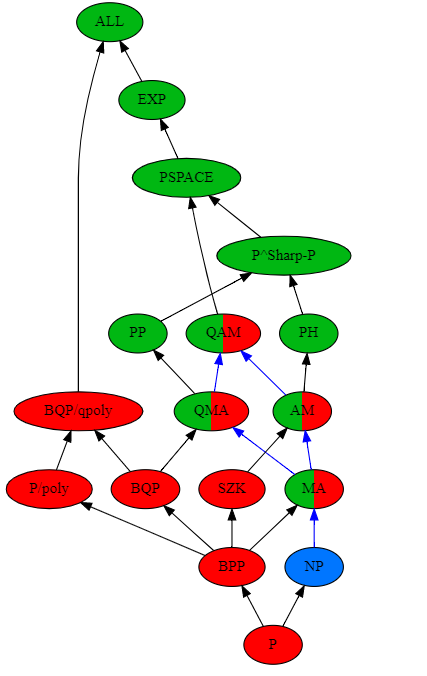
\includegraphics[width=4in]
  {simplified-graph-NP-selected.png}}
  \caption{\label{NP-selected} A sample diagram in the ``all oracles'' world in which 
  $\NP$ is selected. The blue node is selected, a green node indicates that the selected 
  class lies inside the node's class, and a red node indicates that the selected class 
  does not lie inside the node's class. The color on the left side of a node corresponds 
  to the class written in the bubble, while the color on the right corresponds to the 
  complement of the written class. Blue arrows denote containment, while black arrows 
  denote symmetric containment.}
\end{figure}

Finally, a table below the diagram lists alternate names for each complexity
class in $W^*$. In other words, for each class $\sC_1$ that appears in the
diagram, the table lists classes $\sC_1$ for which $\sC_1\subseteq_{W^*}\sC_2$
and $\sC_2\subseteq_{W^*}\sC_1$. Complexity Zoology uses its internal hierarchy
of preferred names to determine which name for a complexity class should appear
in the diagram, choosing arbitrarily between the possibilities having equal
preference.

   \chapter{Complexity Theory Results}

   What follows is a survey of complexity theory that has been aided by the
Complexity Zoology software. It is similar in structure to Scott Aaronson's
Complexity Zoo, although with a much smaller collection of complexity
classes. The role of the software in producing this software has been threefold:
it has identified unanswered questions most useful to creating a complete
picture of the field, it has highlighted redundant information that is the
logical consequence of other data, and it has provided a high-level view of the
current state of knowledge.

Where possible, redundant data has been removed from the survey, although it is 
occasionally left in when it represents a particularly notable or foundational result. 
Results are explained in varying levels of detail with the intent of both providing a
roadmap of complexity theory and illustrating some key arguments and frequently used
techniques. It is hoped that this overview demonstrates the usefulness of a
computer-assisted approach to compiling knowledge about the relationships
between complexity classes.
   \section{Simplified Version} \label{simplified-version}

We begin by considering a simplified version of our survey. In this version,
there are just 17 complexity classes, and we will mostly examine their 
relationships in the world of all oracles.

\subsection{Complexity Classes}\label{class-definitions}

The classes in this mini-survey are listed here in alphabetical order, with
definitions for each.

\begin{itemize}
\item $\msf{ALL}$: The class of all languages. Naturally,
  $\msf{ALL}^f=\{\cL:\cL\subseteq\Sigma^*\}$ for every oracle $f$.
\item $\msf{AM}$: The class of languages computable by the \textit{Arthur-Merlin
    protocol}. Merlin is a \textit{prover} who wants to convince the
  \textit{verifier}, Arthur, that an input $x$ lies in the language
  $\cL$. Merlin knows at the outset whether $x\in\cL$ and can make any argument,
  but he is also biased: he wishes to convince Arthur that $x\in\cL$ regardless
  of whether this is actually true. Arthur, meanwhile, is a polynomial-time
  classical computer. Arthur may use randomness in his calculations, but the
  results of his coin tosses are known to Merlin in advance.

  A language $\cL$ is said to be in $\msf{AM}$ if, when $x\in\cL$, Merlin can
  convince Arthur of this fact with probability $\geq 2/3$, while if
  $x\not\in\cL$, then Merlin cannot convince Arthur that $x\in\cL$ with a
  probability of more than $1/3$. Formally, $\cL\in\msf{AM}^f$ if and only if 
  there exists a polynomial-time Turing machine $M$ with $f$-oracle and 
  functions $p(n),q(n)=\Oh(n^*)$ such that for every $x\in\Sigma^*$,
  \begin{align*}
    x\in\cL&\Longrightarrow\Pr_{y\in\Sigma^{p(|x|)}}[(\exists
    z\in\Sigma^{q(|x|)})[M(x,y,z)=1]]\geq 2/3, \\
    x\not\in\cL&\Longrightarrow\Pr_{y\in\Sigma^{p(|x|)}}[(\exists
    z\in\Sigma^{q(|x|)})[M(x,y,z)=1]]\leq 1/3.  
  \end{align*}
\item $\msf{BPP}$: The class of languages computable in polynomial time, with
  randomness. We can model $\msf{BPP}$ with a special probabilistic Turing
  machine capable of making coin tosses as part of its
  computation. Alternatively, we can make coin tosses in advance and supply the
  result to a deterministic Turing machine as an ancillary string along with
  the input. Formally, $\cL\in\msf{BPP}^f$ if and only if there exists a
  polynomial-time Turing machine $M$ with $f$-oracle and a function
  $p(n)=\Oh(n^*)$ such that for every $x\in\Sigma^*$,
  \[
  \Pr_{y\in\Sigma^{p(|x|)}}[M(x,y)=\cL(x)]\geq 2/3.
  \]
\item $\msf{BQP}$: The class of languages computable in polynomial time by a
  quantum computer. Formally, this means that languages in $\msf{BQP}$ are
  computable by a polynomially sized family of quantum circuits. As discussed in 
  Subsection \ref{quantum-model}, this family must be uniform.
\item $\msf{BQP}/\msf{qpoly}$: $\msf{BQP}$ with quantum polynomial advice. This 
  class consists of languages that can be computed by a polynomial-time quantum 
  computer with polynomial-length \textit{quantum advice}. Quantum advice is a 
  string of qubits that depends only on the length of the input; the qubits are 
  allowed to be in a state of superposition.
\item $\msf{EXP}$: The class of languages computable in
  exponential-time. Formally, $\cL\in\msf{EXP}^f$ if there exists an oracle
  Turing machine $M$ with $f$-oracle that computes $\cL$ in $T(n)$-time with
  $T(n)=\Oh(2^{p(n)})$, where $p(n)=\Oh(n^*)$.
\item $\msf{MA}$: The class of languages computable using the
  \textit{Merlin-Arthur protocol}. This is identical to the Arthur-Merlin
  protocol, except Arthur's coin tosses are unknown to Merlin. Formally,
  $\cL\in\msf{MA}^f$ if there exists a polynomial-time Turing machine $M$ with
  $f$-oracle and functions $p(n),q(n)=\Oh(n^*)$ such that for every $x\in\Sigma^*$,
  \begin{align*}
  x\in\cL&\Longrightarrow(\exists
  z\in\Sigma^{q(|x|)})\left[\Pr_{y\in\Sigma^{p(|x|)}}[M(x,y,z)=1]\geq
  2/3\right], \\
  x\not\in\cL&\Longrightarrow(\forall
  z\in\Sigma^{q(|x|)})\left[\Pr_{y\in\Sigma^{p(|x|)}}[M(x,y,z)=1]\leq 1/3\right].  
  \end{align*}
\item $\msf{NP}$: The class of languages that can be computed by a
  non-deterministic algorithm in polynomial-time. We replace the usual notion of
  a Turing machine with that of a non-deterministic Turing machine with two
  transition functions. Thus, instead of the computational process consisting of
  a sequence of configurations, it consists of a tree of configurations. Then
  $\cL\in\NP$ precisely when if $x\in\cL$, there is a path in the tree that
  accepts the input, while if $x\not\in\cL$, all paths reject. $\NP$ can also be
  defined using deterministic Turing machines with \textit{certificates}:
  formally, $\cL\in\NP^f$ if and only if there exist a polynomial-time oracle
  Turing machine $M$ with $f$-oracle and a function $p(n)=\Oh(n^*)$ such that for
  every $x\in\Sigma^*$,
  \[
  x\in\cL\Longleftrightarrow(\exists y\in\Sigma^{p(|x|)})[M(x,y)=1].
  \]
\item $\sP$: The class of languages that can be computed by a polynomial-time
  Turing machine (or an oracle Turing machine with $f$-oracle in the case of
  $\sP^f$). A polynomial-time Turing machine is one that, on an input of length
  $n$, terminates within $T(n)$ steps, where $T(n)=\Oh(n^*)$.
\item $\sP^{\#\sP}$: $\sP$ with $\#\sP$-oracle. This class consists of languages 
  computable in polynomial time with an oracle $f$ that lies in the function class 
  $\#\sP$. For a pair $(M,p)$ consisting of a polynomial-time Turing machine $M$ 
  and a function $p(n)=\Oh(n^*)$, set
  \[
  Y_{(M,p)}=\{y\in\Sigma^{p(|x|)}:M(x,y)=1\}.
  \]
  Then, $g:\Sigma^*\ra\Sigma^*$ lies in $\#\sP^f$ if and only if there exists a 
  pair $(M,p)$ such that $g(x)=|Y_{(M,p)}|$ for every $x\in\Sigma^*$. Now define 
  $(\sP^{\#\sP})^f=\bigcup_{g\in\#\sP^f}\sP^{g}$.
  
\item $\msf{PH}$: The polynomial hierarchy. For an oracle $f$, define
  $\Sigma_0\sP^f=\sP^f$. Then, for each $j\in\N$, set
  $\Sigma_{j+1}\sP^f=\NP^{\Sigma_j\sP^f}$. Finally, define
  $\msf{PH}=\bigcup_{j=0}^\infty\Sigma_j\sP^f$. We also define $\Pi_j\sP^f$ and
  $\Delta_j\sP^f$ by $\Sigma_0\sP^f=\Delta_0\sP^f=\sP^f$ and
  $\Pi_j\sP^f=\co\NP^{\Sigma_{j-1}\sP^f}$,
  $\Delta_j\sP^f=\sP^{\Sigma_{j-1}\sP^f}$ for $j\geq 1$.
\item $\msf{PP}$: Like $\msf{BPP}$, a class of polynomial-time computable
  languages, with randomness. The defining condition of $\msf{PP}$ is weaker
  than that of $\msf{BPP}$, requiring only that if an input $x$ lies in the
  language, a probabilistic Turing machine obtains the correct answer with a
  probability of at least $1/2$. Formally, $\cL\in\msf{PP}^f$ if and only if
  there exists a polynomial-time Turing machine $M$ with $f$-oracle and a
  function $p(n)=\Oh(n^*)$ such that for every $x\in\Sigma^*$,
  \[
  x\in\cL\Longleftrightarrow\Pr_{y\in\Sigma^{p(|x|)}}[M(x,y)=1]\geq 1/2.
  \]
\item $\sP/\msf{poly}$: $\sP$ with polynomial advice. An \textit{advice string}
  is a fixed string $y_n$ that accompanies an input of length $n$. Being
  \textit{polynomial} advice means that the function $n\mapsto|y_n|$ is
  $\Oh(n^*)$. Formally, $\cL\in(\sP/\poly)^f$ if and only if there exist a
  polynomial-time oracle Turing machine $M$ with $f$-oracle and a function
  $g:\N\mapsto\Sigma^*$, where $|g(n)|=\Oh(n^*)$, such that for every
  $x\in\Sigma^*$,
  \[
  x\in\cL\Longleftrightarrow M(x,g(|x|))=1.
  \]
  Equivalently, $\sP/\poly$ is the class of languages that can be computed by a 
  non-uniform family of polynomial-size classical circuits (see Subsection 
  \ref{classical-models}).
\item $\msf{PSPACE}$: The class of languages that are polynomial-space
  computable. For a function $T:\N\ra\N$, $\cL\in\msf{SPACE}(T(n))^f$ if and
  only if there exist an oracle Turing machine $M$ with $f$-oracle that computes
  $\cL$ and a constant $C$ such that, when $x\in\Sigma^*$ is given as an input
  to the machine, there are at most $CT(|x|)$ cells of each tape that are ever
  written onto during the computation. Then, define
  $\msf{PSPACE}^f=\bigcup_{k=0}^\infty\msf{SPACE}(n^k)^f$. We adopt the convention
  that the space limitation of $\msf{PSPACE}^f$ applies to the oracle tape as 
  well, so that oracle calls are limited to a polynomial of the length of the
  input.
\item $\msf{QAM}$: The class of languages using the quantum 
  Arthur-Merlin protocol. The definition is similar to $\msf{AM}^f$, except $M$ is 
  a polynomial-time quantum computer with $f$-oracle rather than a classical 
  computer, and Merlin is an all-powerful quantum-computer capable of computing any
  system of qubits. Arthur sends Merlin a random string of classical bits, Merlin 
  responds with a polynomial-length quantum message, and then Arthur uses the 
  random bits along with Merlin's message to decide whether to accept or reject the
  input.
\item $\msf{QMA}$: The class of languages using the quantum Merlin-Arthur
  protocol. The definition is the same as $\msf{MA}^f$, except $M$ is a
  polynomial-time quantum computer with $f$-oracle rather than a classical
  computer, and Merlin is an all-powerful quantum-computer. Arthur and Merlin 
  exchange messages in the form of systems of qubits rather than classical bit 
  strings.
\item $\msf{SZK}$: Traditionally defined as the class of languages that can be 
  computed using a statistical zero-knowledge proof protocol, $\msf{SZK}$ can be 
  defined in a simpler way using a special case of this protocol. We call the 
  special case the \textit{rhetorical question protocol}. This is 
  similar to the Arthur-Merlin protocol, except that Arthur's message to Merlin 
  consists of a question for which Arthur has privately computed a correct answer. 
  Arthur accepts the input if and only if Merlin's 
  response matches Arthur's correct answer. Formally, $\cL\in\msf{SZK}^f$ if and 
  only if there exist a polynomial-time oracle Turing machine $M$ with $f$-oracle 
  and a function $p(n)=\Oh(n^*)$ such that for all $x\in\Sigma^*$,
  \begin{align*}
  x\in\cL&\Longrightarrow(\exists P\in\mathcal{M})
  \left[\Pr_{y\in\Sigma^{p(|x|)}}[P(x,M(x,y,0))=M(x,y,1)]\geq 2/3\right], \\
  x\not\in\cL&\Longrightarrow(\forall P\in\mathcal{M})
  \left[\Pr_{y\in\Sigma^{p(|x|)}}[P(x,M(x,y,0))=M(x,y,1)]\leq 1/3\right],
  \end{align*}
  where
  \[
  \mathcal{M}=
  \{P:\Sigma^*\ra\Sigma^*:(\exists q(n)=\Oh(n^*))[P(x)\in\Sigma^{q(|x|)}]\}.
  \]
  See Subsection \ref{szk-subsection} for a discussion of the relationship between 
  this definition of $\msf{SZK}$ and a more conventional definition.
\end{itemize}

\subsection{Inclusions}

To establish the overall structure of the relationships between these 17
complexity classes, we first establish which inclusions are relativizing --
i.e., which inclusions hold for every oracle. To that end, we identify the
symmetric classes, by which we mean the classes $\sC$ such that
$\sC=\cco\cdot\sC$ with respect to every oracle. This will allow us to easily
strengthen many of the inclusions described here. For example, knowing that
$\sP$ is symmetric and that $\sP\subseteq\NP$ for every oracle allows us to
conclude that $\sP\subseteq\cocap\cdot\NP=\NP\cap\co\NP$ with respect to every
oracle.

It is immediate that $\sP$ is symmetric, because a polynomial-time computer can
simply swap its output $\alpha$ with $1-\alpha$. The computer can still perform
this operation if it is quantum, exponential-time, polynomial-space, or has
access to a $\#\sP$-oracle, so $\msf{BQP}$, $\msf{EXP}$, $\msf{PSPACE}$, and
$\sP^{\#\sP}$ are likewise symmetric. A computer receiving advice strings does
not affect this capacity, so $\sP/\poly$ and $\msf{BQP}/\poly$ are symmetric as
well. As was shown in Section \ref{operator-section}, the operators $\cBP$
and $\cP$ commute with $\cco$. Since $\msf{BPP}=\cBP\cdot\sP$ and
$\msf{PP}=\cP\cdot\sP$, it follows that $\msf{BPP}$ and $\msf{PP}$ are
symmetric. Of course, $\msf{ALL}$ is clearly symmetric.

$\msf{PH}$ is symmetric, because $\msf{PH}=\bigcup_{k=0}^\infty\Sigma_k\sP=\bigcup_{k=0}^\infty\Pi_k\sP$. More explicitly:
\begin{lemma}
For every $k\in\N$, $\Delta_k\sP\subseteq\Sigma_k\sP$,
$\Delta_k\sP\subseteq\Pi_k\sP$, $\Sigma_k\sP\subseteq\Delta_{k+1}\sP$, and
$\Pi_k\sP\subseteq\Delta_{k+1}\sP$.
\end{lemma}

\begin{proof}
In the case that $k=0$, $\Delta_k\sP\subseteq\Sigma_k\sP$ because both classes
are equal to $\sP$. If $k>0$, then
$\Delta_k\sP\subseteq\sP^{\Sigma_{k-1}\sP}\subseteq\NP^{\Sigma_{k-1}\sP}=\Sigma_k\sP$.
Since $\Delta_k\sP$ is a symmetric class (being $\sP$ with an oracle), it
follows that $\Delta_k\sP\subseteq\Pi_k\sP$ for every $k$.

For the second pair of inclusions,
$\Delta_k\sP\subseteq\sP^{\Sigma_k\sP}=\Delta_{k+1}\sP$, and then
$\Pi_k\sP\subseteq\Delta_{k+1}\sP$ likewise follows from the symmetry of
$\Delta_{k+1}\sP$.
\end{proof}

$\msf{SZK}$ is a symmetric class:

\begin{theorem}[Okamoto, \cite{okamoto2000relationships}]
$\msf{SZK}=\cco\cdot\msf{SZK}$ with respect to any oracle.
\end{theorem}

Next we discuss which complexity classes are subsets of each other relative to
every oracle. We consider a minimal generating set of inclusions, which in this
context means that all the inclusions will be Hasse relative to the 17 classes
we are considering. In other words, we do not need to prove
$\sP\subseteq\msf{MA}$ because this follows from $\sP\subseteq\NP$ and
$\NP\subseteq\msf{MA}$.

$\sP\subseteq\msf{BPP}$ and $\sP\subseteq\msf{NP}$ are true because both
$\msf{BPP}$ and $\msf{NP}$ are polynomial-time classes, but with additional
powers that can be ignored: to simulate $\sP$ with $\msf{BPP}$, make no coin
tosses; to simulate $\sP$ with $\msf{NP}$, discard the certificate.
Alternatively both inclusions can be said to follow from the properties in
Section \ref{operator-section}, since $\msf{BPP}=\cBP\cdot\sP$ and
$\msf{NP}=\cN\cdot\sP$. Similarly, 
$\msf{BQP}\subseteq\msf{BQP}/\msf{qpoly}$.

As was mentioned during the discussion on the pseudo-operator $\mathpzc{Q}$ in
Section \ref{operator-section}, a quantum computer can perform the same
operations as a classical computer (possibly with the aid of ancilliary qubits).
This applies to probabilistic classic computers as well as deterministic ones,
because a coin flip can be simulated by measuring the qubit
$\frac{1}{\sqrt{2}}(\ket{0}+\ket{1})$. Hence $\msf{BPP}\subseteq\msf{BQP}$. By 
the same principle, $\sP/\poly\subseteq\msf{BQP}/\msf{qpoly}$, 
$\msf{MA}\subseteq\msf{QMA}$, and $\msf{AM}\subseteq\msf{QAM}$.

The inclusion $\msf{BPP}\subseteq\msf{MA}$
is straightforward: in the definition of $\msf{MA}$, the
verifier is a probabilistic polynomial-time Turing machine that must reach the
correct answer with a probability of at least $2/3$. Thus, a protocol in which
Arthur ignores the Merlin and performs his own computations is an
an $\msf{MA}$-protocol that computes a problem in
$\msf{BPP}$. The same argument also shows that $\msf{BQP}\subseteq\msf{QMA}$. 
Similarly, $\msf{BPP}\subseteq\msf{SZK}$. While our definition of $\msf{SZK}$ 
requires that Arthur bases his conclusion on the response given by Merlin, Arthur 
can effectively ``ignore'' Merlin by either telling Merlin the correct answer (if 
Arthur wants to accept the input) or generating a random string as the correct 
answer and sending a blank message to Merlin (if Arthur wants to reject the input).

$\msf{BPP}$ can be \textit{derandomized}, allowing it to be placed inside
$\sP/\poly$.

\begin{theorem}[Adleman, \cite{adleman1978two}]
$\msf{BPP}\subseteq\sP/\poly$ relative to every oracle.
\end{theorem}

\begin{proof}
Let $\cL\in\msf{BPP}$. The class $\msf{BPP}$ is subject to an error-reducing
procedure: by running several copies of a $\msf{BPP}$-machine in parallel and
taking the ``majority vote'' of the machines, we can obtain the correct answer
with a higher probability. Using this technique, we can suppose that there
exists a polynomial-time Turing machine $M$ and a function $p(n)=\Oh(n^*)$ such
that for every $x\in\Sigma^*$,
\[
\Pr_{y\in p(|x|)}[M(x,y)\neq\cL(x)]\leq 1/2^{|x|+1}.
\]
Equivalently, for every $x\in\Sigma^*$ there are at most $2^{p(|x|)-|x|-1}$ 
strings $y\in\Sigma^{p(|x|)}$ such that $M(x,y)\neq\cL(x)$. For $x\in\Sigma^*$, 
set
\[
B_x=\{y\in\Sigma^{p(|x|)}:M(x,y)\neq\cL(x)\},
\]
and for $n\in\N$, set
\[
B_n=\bigcup_{x\in\Sigma^n}B_x.
\]
$B_n$ is the set of ``bad advice'' for an input of length $n$. Now
\[
|B_n|\leq\Sigma_{|x|=n}|B_x|\leq\Sigma_{|x|=n}2^{p(n)-n-1}=2^n2^{p(n)-n-1}=
2^{p(n)-1}<2^{p(n)}=|\Sigma^{p(n)}|,
\]
so the set $\Sigma^{p(n)}\setminus B_n$ is nonempty for every $n$. Thus, there
exists a function $f:\N\ra\Sigma^*$ such that $f(n)\in\Sigma^{p(n)}\setminus
B_n$ for every $n$. We therefore have that for each $x\in\Sigma^*$,
\[
M(x,f(|x|))=\cL(x),
\]
so $\cL\in\sP/\poly$ as desired.
\end{proof}

The fact $\NP\subseteq\msf{MA}$ follows from the observation that replacing the 
definition of $MA$ with a deterministic Turing machine is precisely the 
definition of $\NP$.

We now consider the relationship between $\msf{AM}$ and $\msf{MA}$. To do this, 
we indroduce related (and seemingly different) classes $\msf{AM}[k]$ for 
integers $k\geq 2$. This represents the Arthur-Merlin protocol with $k$ rounds.

\begin{definition}
A $k$-round Arthur-Merlin protocol is an interaction $(V,P)_k$ between a 
probabilistic Turing machine $V$, representing Arthur, and a function 
$P:\Sigma^*\ra\Sigma^*$, representing Merlin. Given an input $x\in\Sigma^*$, 
Arthur computes a message $m_1$ and sends it, along with the random bits $y_1$ 
used in the computation, as a string $\alpha_1=\inner{m_1,y_1}$ to Merlin. 
Merlin responds with a string $\alpha_2$ that is limited in length by a 
polynomial in $|x|$. Arthur sends a new message $\alpha_3=\inner{m_3,y_3}$, 
Merlin responds with $\alpha_4$, and so on, until the sequence 
$(\alpha_1,\ldots,\alpha_k)$ has been generated. Then Arthur deterministically 
computes $V(\alpha_1,\ldots,\alpha_k)$ to decide whether to accept the input. 
We denote the result by $\out_{(V,P)_k}(x)$.

A language $\cL$ lies in $\msf{AM}[k]$ if and only if there exists a 
polynomial-time Turing machine $V$ such that for every $x\in\Sigma^*$,
\begin{align*}
x\in\cL&\Longrightarrow
(\exists P\in\mathcal{M})\Pr[\out_{(V,P)_k}(x)=1]\geq 2/3, \\
x\not\in\cL&\Longrightarrow
(\forall P\in\mathcal{M})\Pr[\out_{(V,P)_k}(x)=1]\leq 1/3,
\end{align*}
where
\[
\mathcal{M}=\{P:\Sigma^*\rightarrow\Sigma^*:(\exists 
q(n)=\Oh(n^*))[P(x)\in\Sigma^{q(|x|)}]\}.
\]
\end{definition}
With this definition, we obtain $\msf{AM}=\msf{AM}[2]$. Moreover, Arthur can 
imitate the Merlin-Arthur protocol within a 3-round Arthur-Merlin protocol: 
after sending his message to Merlin and receiving a response, Arthur makes his 
final computation with a fresh set of random bits. These bits are sent to 
Merlin, but since Merlin cannot send a second response, these random bits are 
effectively private. Hence $\msf{MA}\subseteq\msf{AM}[3]$.

As it turns out, however, adding extra rounds to an Arthur-Merlin protocol does 
not change the computational power of $\msf{AM}$:
\begin{theorem}[Babai, \cite{babai1985trading}]
$\msf{AM}[k+1]\subseteq\msf{AM}[k]$ with respect to any oracle for all integers 
$k\geq 2$.
\end{theorem}
$\msf{AM}[2]\subseteq\msf{AM}[3]\subseteq\msf{AM}[4]\subseteq\ldots$, since Arthur 
can choose to ignore the later rounds of his interaction with Merlin. Hence 
$\msf{AM}=\msf{AM}[k]$ for every $k$.

As an immediate corollary of $\msf{MA}\subseteq\msf{AM}[3]$ and the above 
theorem, we deduce $\msf{MA}\subseteq\msf{AM}$. These arguments are not 
affected if Arthur is quantum rather than classical, so we also have 
$\msf{QMA}\subseteq\msf{QAM}$. Okamoto \cite{okamoto2000relationships} showed that 
$\msf{SZK}$ could be characterized by a constant-round protocol with a public-coin 
Arthur; it follows that $\msf{SZK}\subseteq\msf{AM}$.

To see that $\msf{AM}\subseteq\msf{PH}$, we need an alternate characterization 
of $\msf{PH}$:
\begin{lemma}
For every language $\cL\subseteq\Sigma^*$, $\cL\in\Sigma_k\sP$ if and only if 
there exists a polynomial-time Turing machine $M$ and 
$p_1(n),\ldots,p_k(n)=\Oh(n^*)$ such that for all $x\in\Sigma^*$,
\[
x\in\cL\Longleftrightarrow
(Q_1 y_1\in p_1(|x|))\ldots(Q_k y_k\in p_k(|x|))
[M(x,y_1,\ldots,y_k)=1],
\]
where $Q_j$ is $\exists$ when $j$ is odd and $\forall$ when $j$ is even.
\end{lemma}
\begin{proof}
Denote this alternative version of $\Sigma_k\sP$ by $\bar\Sigma_k\sP$, and 
denote $\bar\Pi_n\sP=\cco\cdot\bar\Sigma_k\sP$. If $k=0$, then 
$\Sigma_0\sP=\bar\Sigma_0\sP=\sP$. Thus, we can suppose for induction that 
$\Sigma_{k+1}\sP=\bar\Sigma_{k+1}\sP$. We have
\[
\bar\Sigma_{k+1}\sP=\cN\cdot\bar\Pi_k\sP=\cN\cdot\Pi_k\sP\subseteq
\cN\cdot\sP^{\Pi_k\sP}=\cN\cdot\sP^{\Sigma_k\sP}=\NP^{\Sigma_k\sP}=
\Sigma_{k+1}\sP,
\]
so it suffices to show that $\Sigma_{k+1}\sP\subseteq\bar\Sigma_{k+1}\sP$.

Suppose $\cL\in\Sigma_{k+1}\sP$. Then there exists a polynomial-time Turing 
machine $M$ with $f$-oracle, where $f\in\Sigma_k\sP$, and a function 
$p(n)=\Oh(n^*)$ such that
\begin{equation}\label{PH1}
x\in\cL\Longleftrightarrow
(\exists y\in\Sigma^{p(|x|)})[M(x,y)=1]
\end{equation}
for every $x\in\Sigma^*$. On an input $\inner{x,y}$, the machine makes $q(|x|)$ 
oracle calls, where $q(n)=\Oh(n^*)$. Let $M^\prime$ be the polynomial-time Turing 
machine such that $M^\prime(x,y,a_1,\ldots,a_{q(|x|)})$ computes $M(x,y)$ when 
$a_1,\ldots,a_{q(|x|)}$ are given as oracle replies. Then (\ref{PH1}) can be 
written as 
\begin{equation}
x\in\cL\Longleftrightarrow
(\exists y\in\Sigma^{p(|x|)},a_1,\ldots,a_{q(|x|)}\in\Sigma^{q(|x|)})
[M^\prime(x,y,a_1,\ldots,a_{q(|x|)})\AND a_1,\ldots,a_{q(|x|)}\text{ are 
correct}].
\end{equation}\label{PH2}
"Correct" means that, if $M$ queries the oracle with $z$, the oracle responds 
with $f(z)$. It is enough to show that ``$a_1,\ldots,a_{q(|x|)}$ are correct'' 
is a $\bar\Sigma_{k+1}\sP$ predicate, because then the entire right side of 
(\ref{PH2}) is a $\bar\Sigma_{k+1}\sP$ predicate. To see that this is the case, 
note that given $x$, $y$, and $a_1,\ldots,a_{q(|x|)}$, we can complete the 
queries $z_1,\ldots,z_{q(|x|)}$ given to the oracle in polynomial time (let 
$M^\prime$ run, and then record the oracle queries as they occur). Then 
``$a_1,\ldots,a_{q(|x|)}$ are correct'' is equivalent to
\[
\bigwedge_{j=1}^{q(|x|)}[A(z_j)=a_j],
\]
which is a conjunction of $\Oh(|x|^*)$-many $\bar\Sigma_{k+1}\sP$ predicates 
(specifically, $(z_j)=1$ is a $\bar\Sigma_k$ predicate, and $f(z_j)=0$ is a 
$\bar\Pi_k$ predicate) and therefore a $\bar\Sigma_{k+1}\sP$ predicate itself. 
Hence $\cL\in\bar\Sigma_{k+1}\sP$ as desired.
\end{proof}
We also need the following result:
\begin{theorem}[Sipser-G\`acs-Lautemann]
If $\cL\in\cBP\cdot\sC$ for a complexity class $\sC$, there exist
$\cL^\prime\in\sC$ and functions $p(n),q(n)=\Oh(n^*)$ such that
\[
x\in\cL\Longleftrightarrow
(\exists u_1,\ldots, u_{p(|x|)}\in\Sigma^{q(|x|)})
(\forall r\in\Sigma^{q(|x|)})
\left[\bigvee_{j=1}^{p(|x|)}\inner{x,r+_2u_j}\in\cL^\prime\right],
\]
where $+_2$ denotes entrywise addition modulo 2.
\end{theorem}
\begin{proof}
Let $\cL\in\cBP\cdot\sC$. By the same error-reduction procedure used in the
proof of $\msf{BPP}\subseteq\sP/\poly$, there exists a language 
$\cL^\prime\in\sC$ and a function $p(n)=\Oh(n^*)$ such that for every 
$x\in\Sigma^*$,
\begin{align}
\label{SGL1} x\in\cL&\Longrightarrow
\Pr_{y\in\Sigma^{p(|x|)}}[\inner{x,y}\in\cL^\prime]\geq 1-2^{-|x|}, \\ 
\label{SGL2} x\not\in\cL&\Longrightarrow
\Pr_{y\in\Sigma^{p(|x|)}}[\inner{x,y}\in\cL^\prime]\leq 2^{-|x|}. 
\end{align}
For each $x\in\Sigma^*$, set
\[
A_x=\{y\in\Sigma^{p(|x|)}:\inner{x,y}\in\cL^\prime\}.
\]
Then (\ref{SGL1}) and (\ref{SGL2}) can be rewritten as
\begin{align}
\label{SGL1P} x\in\cL&\Longrightarrow
|A_x|\geq 2^{p(|x|)}(1-2^{-|x|}), \\ 
\label{SGL2P} x\not\in\cL&\Longrightarrow
|A_x|\leq 2^{p(|x|)-|x|}.
\end{align}
Now for $m\in\N$, $S\subseteq\Sigma^m$, and $u\in\Sigma^m$, set
\[
S+_2u=\{y+_2u:y\in S\}.
\]
Note that for any $n\in\N$, if $S\subseteq\Sigma^{p(n)}$ satisfies $|S|\leq 
2^{p(n)-n}$, then for any $u_1,\ldots,u_k\in\Sigma^{p(n)}$ with $k<2^n$, we have
\[
\left|\bigcup_{j=1}^k(S+_2u_j)\right|\leq
\sum_{j=1}^k|S+_2u_j|=k|S|\leq k2^{p(n)-n}<2^{p(n)},
\]
so that $\bigcup_{j=1}^k(S+_2u_j)\neq\Sigma^{p(|x|)}$. In particular, if we set 
$q(n)=\lceil p(n)/n)\rceil+1$ for every $n\in\N$ (we will need the fact that 
$p(n)<nq(n)$ shortly), then it follows from 
(\ref{SGL2P}) that
\begin{equation}\label{SGL3}
x\not\in\cL\Longrightarrow
(\forall u_1,\ldots,u_{q(|x|)}\in\Sigma^{p(|x|)})
\left[\bigcup_{j=1}^{q(|x|)}(A_x+_2u_j)\neq\Sigma^{p(|x|)}\right].
\end{equation}
On the other hand, suppose that $S\subseteq\Sigma^{p(|x|)}$ satisfies 
$|S|\geq 2^{p(n)}(1-2^{-n})$. Let $u_1,\ldots,u_{q(n)}\in\Sigma^{p(n)}$ be 
chosen uniformly randomly. Then $r+_2u_j$ is also randomly chosen for any 
partucular $r$, and we can compute as follows:
\begin{align*}
\Pr\left[\bigcup_{j=1}^{q(n)}(S+_2u_j)\neq\Sigma^{p(n)}\right]
&=\Pr\left[(\exists r\in\Sigma^{p(n)})\left[r\not\in\bigcup_{j=1}^{q(n)}
(S+_2u_j)\right]\right] \\
&=\Pr\left[(\exists r\in\Sigma^{p(n)})\left[\bigvee_{j=1}^{q(n)}r\not\in
S+_2u_j\right]\right] \\
&=\Pr\left[(\exists r\in\Sigma^{p(n)})\left[\bigvee_{j=1}^{q(n)}r+_2u_j\not\in
S\right]\right] \\
&=\Pr\left[\bigvee_{j=1}^{q(n)}u_j\not\in S\right]
=\prod_{j=1}^{q(n)}\Pr[u_j\not\in S]
\leq\prod_{j=1}^{q(n)}2^{-n}
=2^{-nq(n)}<2^{-p(n)}<1.
\end{align*}
Hence $\Pr[\bigcup_{j=1}^{q(n)}(S+_2u_j)=\Sigma^{p(n)}]>0$, and so it follows 
from (\ref{SGL1P}) that
\begin{equation} \label{SGL4}
x\in\cL\Longrightarrow(\exists u_1,\ldots,u_{q(|x|)}\in\Sigma^{p(|x|)})
\left[\bigcup_{j=1}^{q(|x|)}(A_x+u_j)=\Sigma^{p(|x|)}\right].
\end{equation}
(\ref{SGL3}) and (\ref{SGL4}) together are equivalent to the desired result.
\end{proof}
\begin{corollary}
$\msf{AM}\subseteq\Pi_2\sP$ with respect to every oracle.
\end{corollary}
\begin{proof}
The definition of $\msf{AM}$ gives $\msf{AM}=\cBP\cdot\NP$ and hence 
$\cco\cdot\msf{AM}=\cBP\cdot\co\NP$. Thus, by the previous theorem, for 
$\cL\in\cco\cdot\msf{AM}$ there exist $\cL^\prime\in\co\NP$ and 
$p(n),q(n)=\Oh(n^*)$ such that
\[
x\in\cL\Longleftrightarrow
(\exists u_1,\ldots, u_{p(|x|)}\in\Sigma^{q(|x|)})
(\forall r\in\Sigma^{q(|x|)})
\left[\bigvee_{j=1}^{p(|x|)}\inner{x,r+_2u_j}\in\cL^\prime\right]
\]
for every $x\in\Sigma^*$. It follows that $\cL\in\Sigma_2\sP$ by the quantifier 
definition of $\Sigma_2\sP$. Therefore, $\cco\cdot\msf{AM}\subseteq\Sigma_2\sP$.
\end{proof}
We next have $\msf{QMA}\subseteq\msf{PP}$ \cite{vyalyi2003qma} with respect to 
every oracle. In fact, $\msf{QMA}\subseteq\msf{A}_0\msf{PP}$, where 
$\msf{A}_0\msf{PP}\subseteq\msf{PP}$ is a class defined as follows: for 
$\cL\subseteq\Sigma^*$, we say $\cL\in\msf{A}_0\msf{PP}$ if and only if there 
exist functions $f,g:\Sigma^*\ra\Sigma^*$, where $g$ is polynomial-time 
computable and
\[
f(x)=|\{y\in\Sigma^{p(|x|)}:M(x,y)=1\}|-|\{y\in\Sigma^{p(|x|)}:M(x,y)=0\}|
\]
for a polynomial-time Turing machine $M$ and $p(n)=\Oh(n^*)$, such that for every 
$x\in\Sigma^*$,
\begin{align*}
x\in\cL&\Longrightarrow f(x)>g(x), \\
x\not\in\cL&\Longrightarrow f(x)<g(x)/2.
\end{align*}
We now consider the class $\sP^{\#\sP}$. $\#\sP$ can be considered to be 
the function class analogue of $\msf{PP}$ in the same way that $\msf{FP}$, the 
class of polynomial-time computable functions, is the function class analogue 
of $\sP$. In general, including a $\sP$-oracle in a computational process is 
equivalent to including an $\msf{FP}$-oracle, because with a $\sP$-oracle one 
can determine the output $f(x)$ of a function $f\in\msf{FP}$ by successively 
computing each bit of $f(x)$. Similarly, a $\msf{PP}$-oracle can be used to 
determine each bit of the output of a function in $\#\sP$, thereby simulating a 
$\#\sP$-oracle. Hence $\sP^{\#\sP}=\sP^{\msf{PP}}$. It follows that 
$\msf{PP}\subseteq\sP^{\#\sP}$ (this only requires the straightforward direction
$\sP^{\msf{PP}}\subseteq\sP^{\#\sP}$).

$\sP^{\#\sP}$ also contains the polynomial hierarchy:
\begin{theorem}[Toda, \cite{toda1991pp}]
$\msf{PH}\subseteq\sP^{\#\sP}$ relative to every oracle.
\end{theorem}
Another inclusion that makes use of an intermediate class is 
$\msf{QAM}\subseteq\msf{PSPACE}$.
\begin{theorem}[\cite{marriott2005quantum}]
$\msf{QAM}\subseteq\cBP\cdot\msf{PP}$ relative to every oracle.
\end{theorem}
Now $\cBP\cdot\msf{PP}\subseteq\msf{PSPACE}$.
\begin{lemma}
$\msf{PP}\subseteq\msf{PSPACE}$.
\end{lemma}
\begin{proof}
Since $\msf{PSPACE}$ is not limited in computational time, given a 
polynomial-time Turing machine $M$ and a function $p(n)=\Oh(n^*)$, a 
$\msf{PSPACE}$-machine can simulate a $\msf{PP}$-machine by keeping a tally of 
how many $y\in\Sigma^{p(|x|)}$ satisfy $M(x,y)=1$ for the input $x$.
\end{proof}
This derandomization also applies to the probabilistic version of 
$\msf{PSPACE}$.
\begin{lemma}
$\cBP\cdot\msf{PSPACE}\subseteq\msf{PSPACE}$.
\end{lemma}
It now follows that
\[
\msf{QAM}\subseteq\cBP\cdot\msf{PP}\subseteq\cBP\cdot\msf{PSPACE}\subseteq
\msf{PSPACE}.
\]
With one additional lemma, we can also prove that 
$\sP^{\#\sP}\subseteq\msf{PSPACE}$.
\begin{lemma}
If $\cL\in\msf{PSPACE}$, then $\msf{PSPACE}^\cL\subseteq\msf{PSPACE}$.
\end{lemma}
\begin{proof}
By our convention, oracle calls are limited in length to a polynomial of the imput.
Hence any calls to the oracle in a $\msf{PSPACE}^\cL$-machine can be replaced with 
a direct computation of $\cL(x)$ by a $\msf{PSPACE}$-machine.
\end{proof}
Now
\[
\sP^{\#\sP}\subseteq\sP^{\msf{PP}}\subseteq\msf{PSPACE}^{\msf{PSPACE}}\subseteq
\msf{PSPACE}.
\]
For our final $\msf{PSPACE}$ inclusion, observe that a $\msf{PSPACE}$-machine is
limited to $2^{p(n)}$ possible configurations for an input of length $n$, where 
$p(n)=\Oh(n^*)$. Thus, any computation that halts must do so within $2^{p(n)}$ 
steps. Therefore $\msf{PSPACE}\subseteq\msf{EXP}$.

The results of this subsection are summarized in Figure 
\ref{fig:mini-zoo-inclusion}.

\begin{figure}[!htb]
  \center{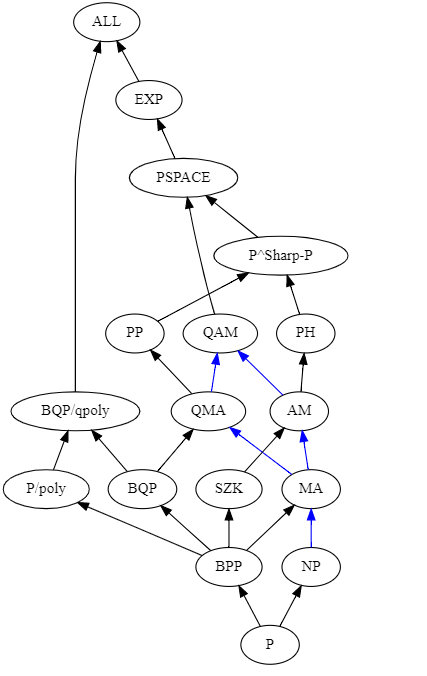
\includegraphics[width=4in]
  {simplified-graph-uncolored.png}}
  \caption{\label{fig:mini-zoo-inclusion} Inclusions that hold with respect to 
  every oracle for 17 complexity classes. Blue indicates that the lower class is 
  included in the upper class. Black indicates that the lower class and its 
  complement are included in the upper class.}
\end{figure}

\subsection{Oracle Separations and Collapses}

Now we present some of the inclusions that fail for some oracle, as well as some 
inclusions that do not relativize. As far as relativizing inclusions are 
concerned, the picture presented in Figure \ref{fig:mini-zoo-inclusion} is 
complete for the 17 complexity classes shown. We cannot, for instance, show that 
$\sP/\poly$ is contained in $\msf{BQP}$ or that $\msf{EXP}$ is contained in $\sP$
for every oracle. These particular examples hold for every oracle: in the former 
case because $\msf{BQP}$ is countable while $\sP/\poly$ is not, and in the latter
case because of the \textit{time-hierarchy theorem}.

For functions $f,g:\N\ra\N$, we write $f(n)=o(g(n))$ if $f(n)/g(n)\ra 0$ as 
$n\ra\infty$. Denote by $\msf{DTIME}(T(n))$ the class of languages that are 
computable in $T(n)$-time.

\begin{theorem}[Time-hierarchy theorem]
If $f,g:\N\ra\N$ satisfy $f(n)\log f(n)=o(g(n))$, then
\[
\msf{DTIME}(f(n))\subsetneq\msf{DTIME}(g(n))
\]
with respect to every oracle.
\end{theorem}
\begin{proof}
The technique used to prove this theorem is \textit{diagonalization}, inspired by
the set theoretic method of the same name. Since $g(n)$ grows much faster than 
$f(n)\log f(n)$, we have that $\msf{DTIME}(f(n))\subseteq\msf{DTIME}(g(n))$. It 
remains to show that $\msf{DTIME}(g(n))\not\subseteq\msf{DTIME}(f(n))$.

Let $U$ indicate the universal Turing machine of Theorem \ref{universal-machine}.
We carry out the following procedure: on input $x$, compute $M_x(x)$ on a 
suitable universal TM for $g(|x|)$ steps, where $M_x$ is the Turing machine 
encoded by $x$. If the computation finishes, output $1-M_x(x)$. Otherwise, output
$0$. Let $D$ be the Turing machine that follows this algorithm. By the choice of 
universal Turing machine and the fact that $f(n)\log f(n)=o(g(n))$, we have 
$D\in\msf{DTIME}(g(n))$.

Next, assume the language determined by $D$ lies in  $\msf{DTIME}(f(n))$. Then, 
there exists a Turing $M$ that decides the same language in $\Oh(f(n))$-time. Then
$M$ has some encoding, and in fact can be assumed to have infinitely many 
encodings, so we fix some encoding $y$ that is long enough so that $f(|y|)\log 
f(|y|)$ is much less than $g(|y|)$. Then the universal Turing machine can simulate
$M_y$ on input $y$ within $g(|y|)$ steps, and so $D(y)=1-M_y(y)=1-M(y)$, 
contradicting the assumption that $D(y)=M(y)$. Therefore, 
$\msf{DTIME}(g(n))\not\subseteq\msf{DTIME}(f(n))$.
\end{proof}

The time-hierarchy theorem proves that there is no oracle collapse from 
$\msf{EXP}$ to $\sP$. There is, however, an oracle collapse from $\msf{PSPACE}$ to
$\sP$; i.e., there is an oracle relative to which $\sP=\msf{PSPACE}$. The usual 
method to make use of a $\msf{PSPACE}$-complete problem---a language $\cL$ in 
$\msf{PSPACE}$ such that every other question in $\msf{PSPACE}$ can be reduced to 
the question of whether $y\in\cL$, where $y$ can be computed from the input in 
polynomial time. Then an oracle for $\cL$ does not give $\msf{PSPACE}$ any 
additional computational power, while boosting $\sP$ up to $\msf{PSPACE}$. 
However, in Section \ref{ah-plo-subsection} we will show that 
there is an even larger class that collapses to $\sP$.

Such a collapse also shows that there is an oracle relative to which $\sP=\NP$. 
There is also an oracle relative to which $\sP\neq\NP$, which establishes that no 
relativizing proof can settle the $\sP$ versus $\NP$ question. A \textit{password oracle} is a type of oracle $f$ constructed so that
$\sC_1^f\not\subseteq\sC_2^f$. Typically, $f$ is a function
$\Sigma^*\times\Sigma^*\rightarrow\Sigma^*$ chosen so that
$PW_f=\{x\in\Sigma:P\}$ lies in $\sC_1^f$ but not in $\sC_2^f$, where $P$ is a
proposition depending on the values of $f(x,y)$ for $y\in\Sigma^*$ (the
\textit{passwords} of $x$). The oracle $f$ can be adversarially constructed or,
in many cases, selected according to a random process.

\begin{theorem}
Let $f:\Sigma^{2*}\ra\Sigma\cup\{\square\}$ be a function selected randomly
according to the following rules:
\begin{itemize}
\item For every $x\in\Sigma^n$, there exists a unique $y\in\Sigma^n$ such that
$f(x,y)\neq\square$. This $y$ is selected using the uniform distribution on
$\Sigma^n$.
\item  For every $x\in\Sigma^n$, if $y$ is the unique element of $\Sigma^n$ such
that $f(x,y)\neq\square$, then $\Pr[f(x,y)=1]=\Pr[f(x,y)=0]=1/2$.
\end{itemize}
Then $(\cocap\cdot\msf{NP})^f\not\subseteq(\sP/\poly)^f$ with probability 1.
\end{theorem}

\begin{proof}
For each $x\in\Sigma^*$, define $PW_f(x)=f(x,y)$, where $y$ is the unique
element of $\Sigma^{|x|}$ such that $f(x,y)\neq\square$. Then
$PW_f\in(\cocap\cdot\msf{NP})^f$, because for a given $x\in\Sigma^*$ the unique
$y$ can be used as the certificate to check that $PW_f(x)=1$ or $PW_f(x)=0$.

Fix an enumeration $\{M_k\}$ of Turing machines. For $M_k$ and input of length
$n$, we allow computation times up to $C_kn^{r_k}$ and advice strings up to
length $D_kn^{s_k}$, where the coefficients and exponents are unbounded and
increasing as functions of $k$. Then, since for any $x\in\Sigma^n$ there are
$2^n$ possible values of $y$, while advice and computation time are polynomials
of $n$, we have
\[
\Pr[(\forall n)(\exists\text{ advice }a)(\forall|x|=n)[M_k(x,a)=PW_f(x)]]=0.
\]
\end{proof}

The above proof actually establishes the stronger claim that 
$(\cocap\cdot\msf{UP})^f\not\subseteq(\sP/\poly)^f$, where $\msf{UP}$ denotes 
\textit{unambiguous polynomial time} (see Subsection \ref{up-section}).
   \section{Overview of the Complexity Zoology Data Set}

This section enumerates the complexity classes, inclusions, and oracle separations
of Complexity Zoology's data set. The data is listed in the same order as in the 
data itself: alphabetically by complexity class, with relations listed under the 
class that appears on the left side of the relation. As a result, many classes are
discussed before the subsection in which they are defined. Some trivial inclusions
are omitted. Statements of equality appear under the less preferred name for the 
class. Large parts of this data set, especially those inclusions that are 
considered to be open, are based on email and in-person communication with Scott 
Aaronson and Lance Fortnow.

Complexity Zoology studies the relationships between complexity classes in six 
different modal worlds: all oracles, all algebraic oracles, some algebraic 
oracle, the random oracle, the trivial oracle, and some oracle. The data set 
would be considered complete when each possible inclusion is settled as true, 
false, or open in each of these six worlds. The current status of the data set is 
shown in Table \ref{data-status}. Note that the trivial world is complete (i.e., 
there are no unknown inclusions).

\begin{table}[]
\begin{tabular}{lllllll}
World:                & P     & D    & O    & UP  & UD   & UU   \\ \hline
All oracles           & 3680  & 9354 & 460  & 20  & 417  & 111  \\
All algebraic oracles & 3022  & 3332 & 326  & 0   & 3918 & 114  \\
Some algebraic oracle & 3022  & 2185 & 0    & 326 & 0    & 5179 \\
Random oracle         & 2435  & 5405 & 1058 & 508 & 156  & 140  \\
Trivial oracle        & 2566  & 2021 & 4725 & 0   & 0    & 0    \\
Some oracle           & 11344 & 2542 & 0    & 156 & 0    & 0   
\end{tabular}
\caption{\label{data-status} The current status of the Complexity Zoology data 
set. This table shows the number of inclusions of each type that exist for each 
world. P indicates \textit{proven}, D indicates \textit{disproven}, O indicates 
\textit{open}, UP indicates \textit{unknown but provable}, and UU indicates 
\textit{unknown with no further data}. The terms \textit{unknown}, 
\textit{provable}, and \textit{disprovable} are explained in Sections 
\ref{zoology-logic} and \ref{extremal-unknowns}.}
\end{table}

\begin{figure}[htb]
  \center{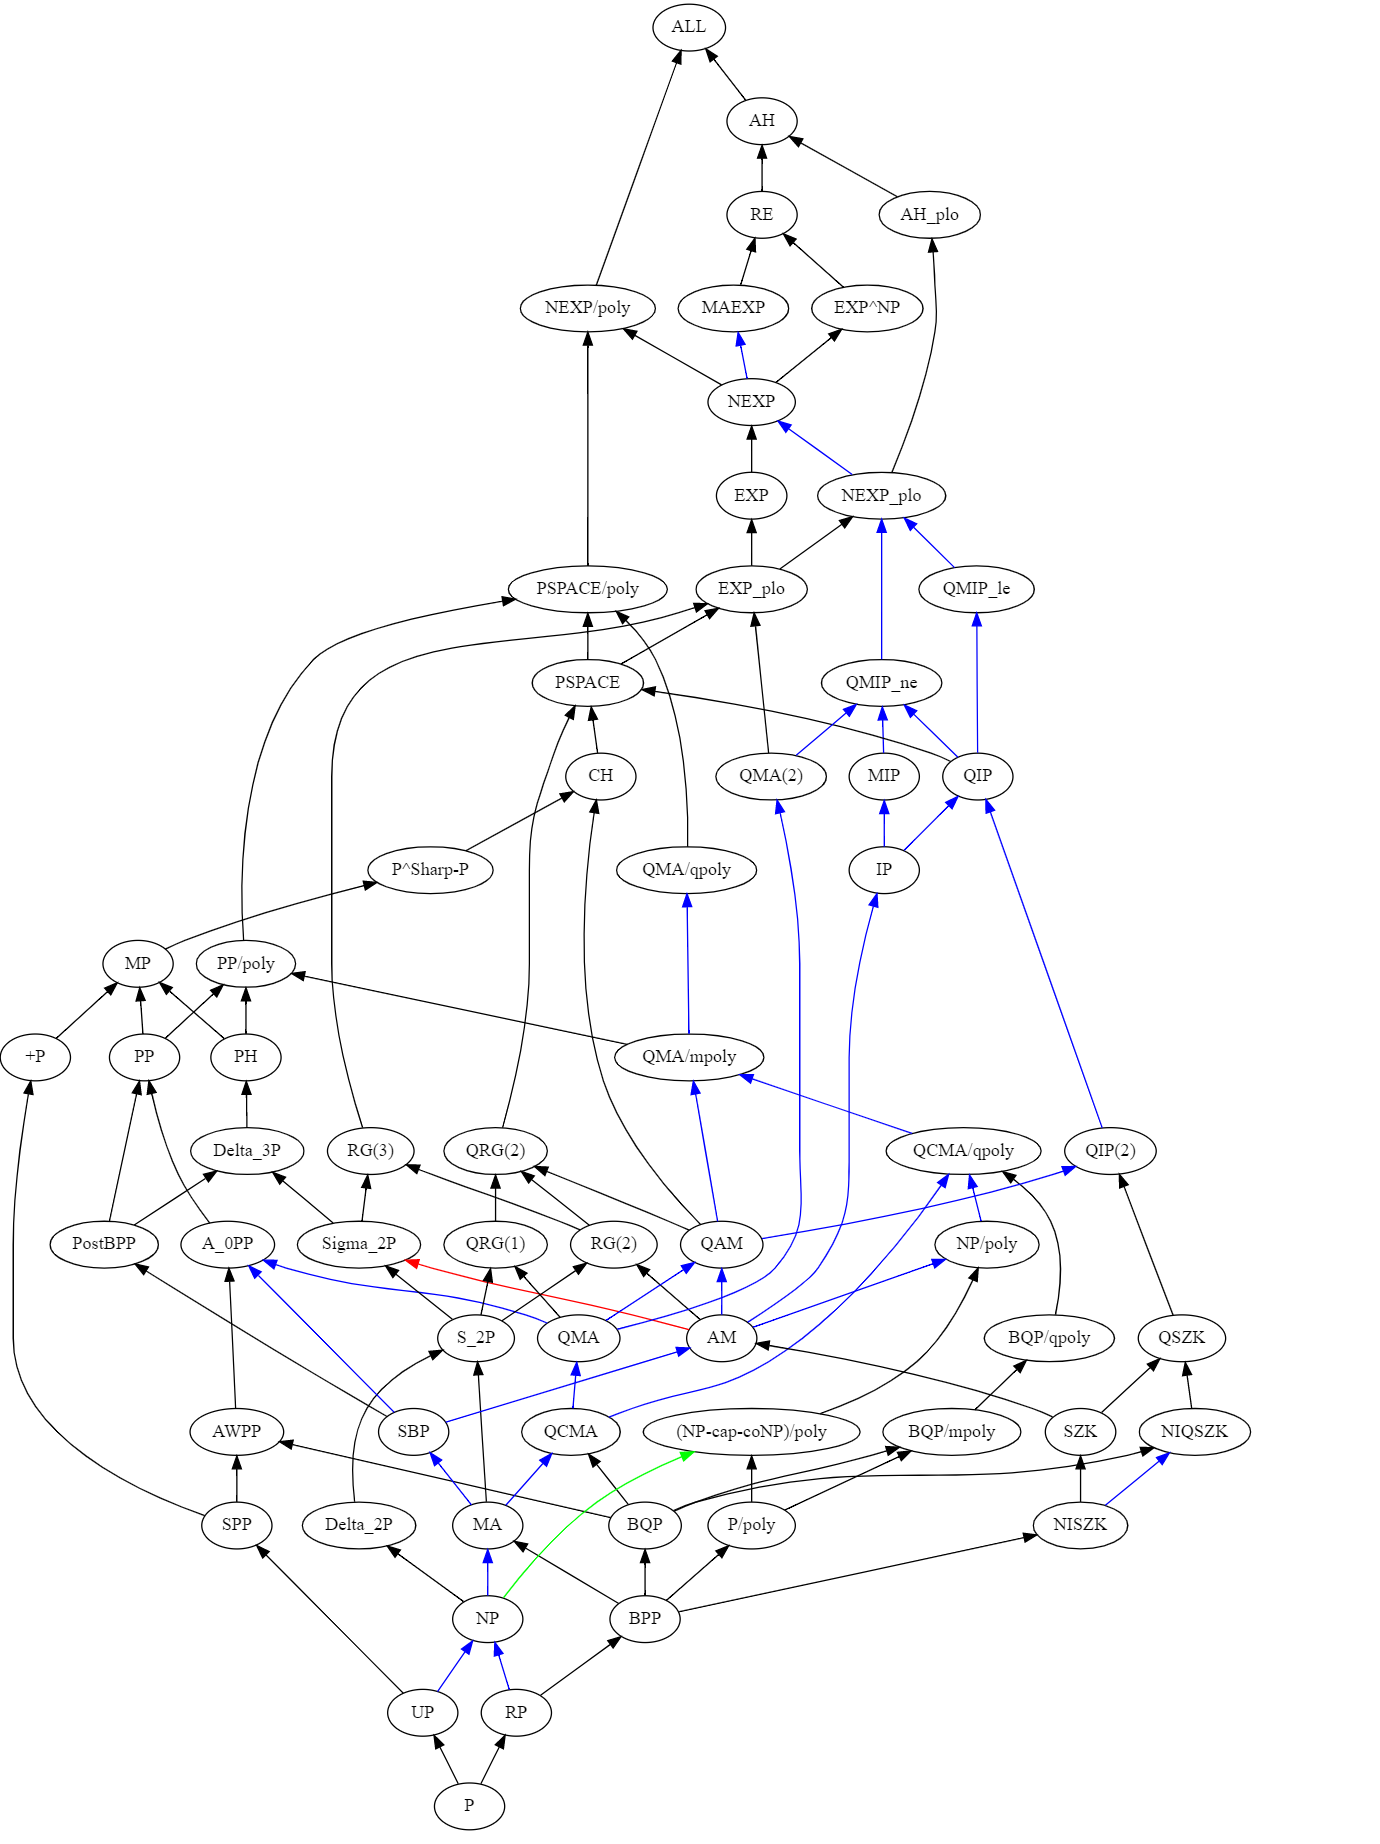
\includegraphics[height=7.7in]
  {all-oracles-full.png}}
  \caption{\label{fig:mini-zoo-inclusion} Inclusions that hold with respect to 
  every oracle. Blue arrows denote containment, black arrows denote symmetric 
  containment, red arrows indicate that the complement of the first class is contained 
  in the second, and green arrows indicate that the intersection of the first class with
  its complement is contained in the second class.}
\end{figure}

\begin{figure}[htb]
  \center{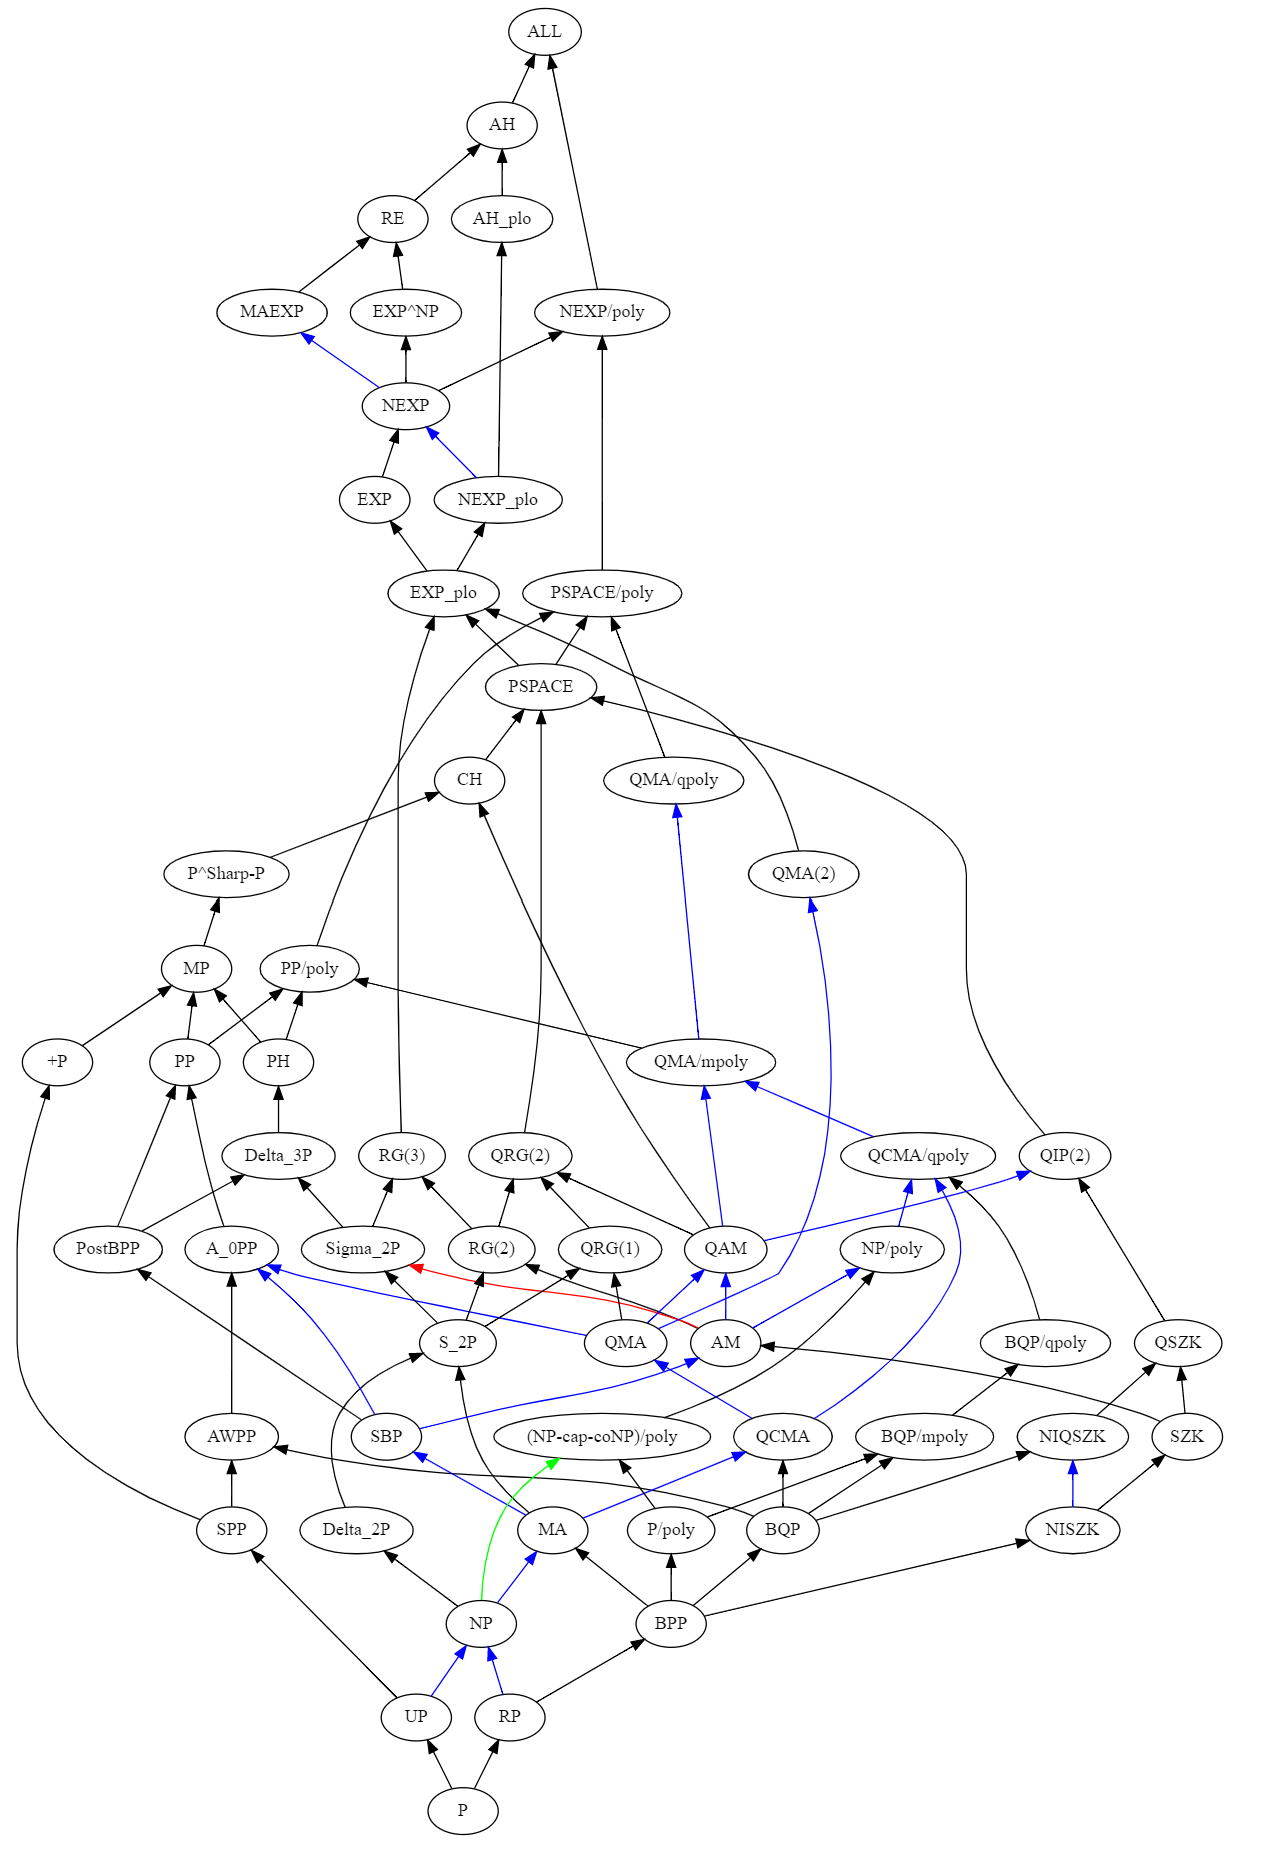
\includegraphics[height=8in]
  {algebraic-oracles-full.png}}
  \caption{\label{fig:mini-zoo-inclusion} Inclusions that hold with respect to 
  all algebraic oracles.}
\end{figure}

\begin{figure}[htb]
  \center{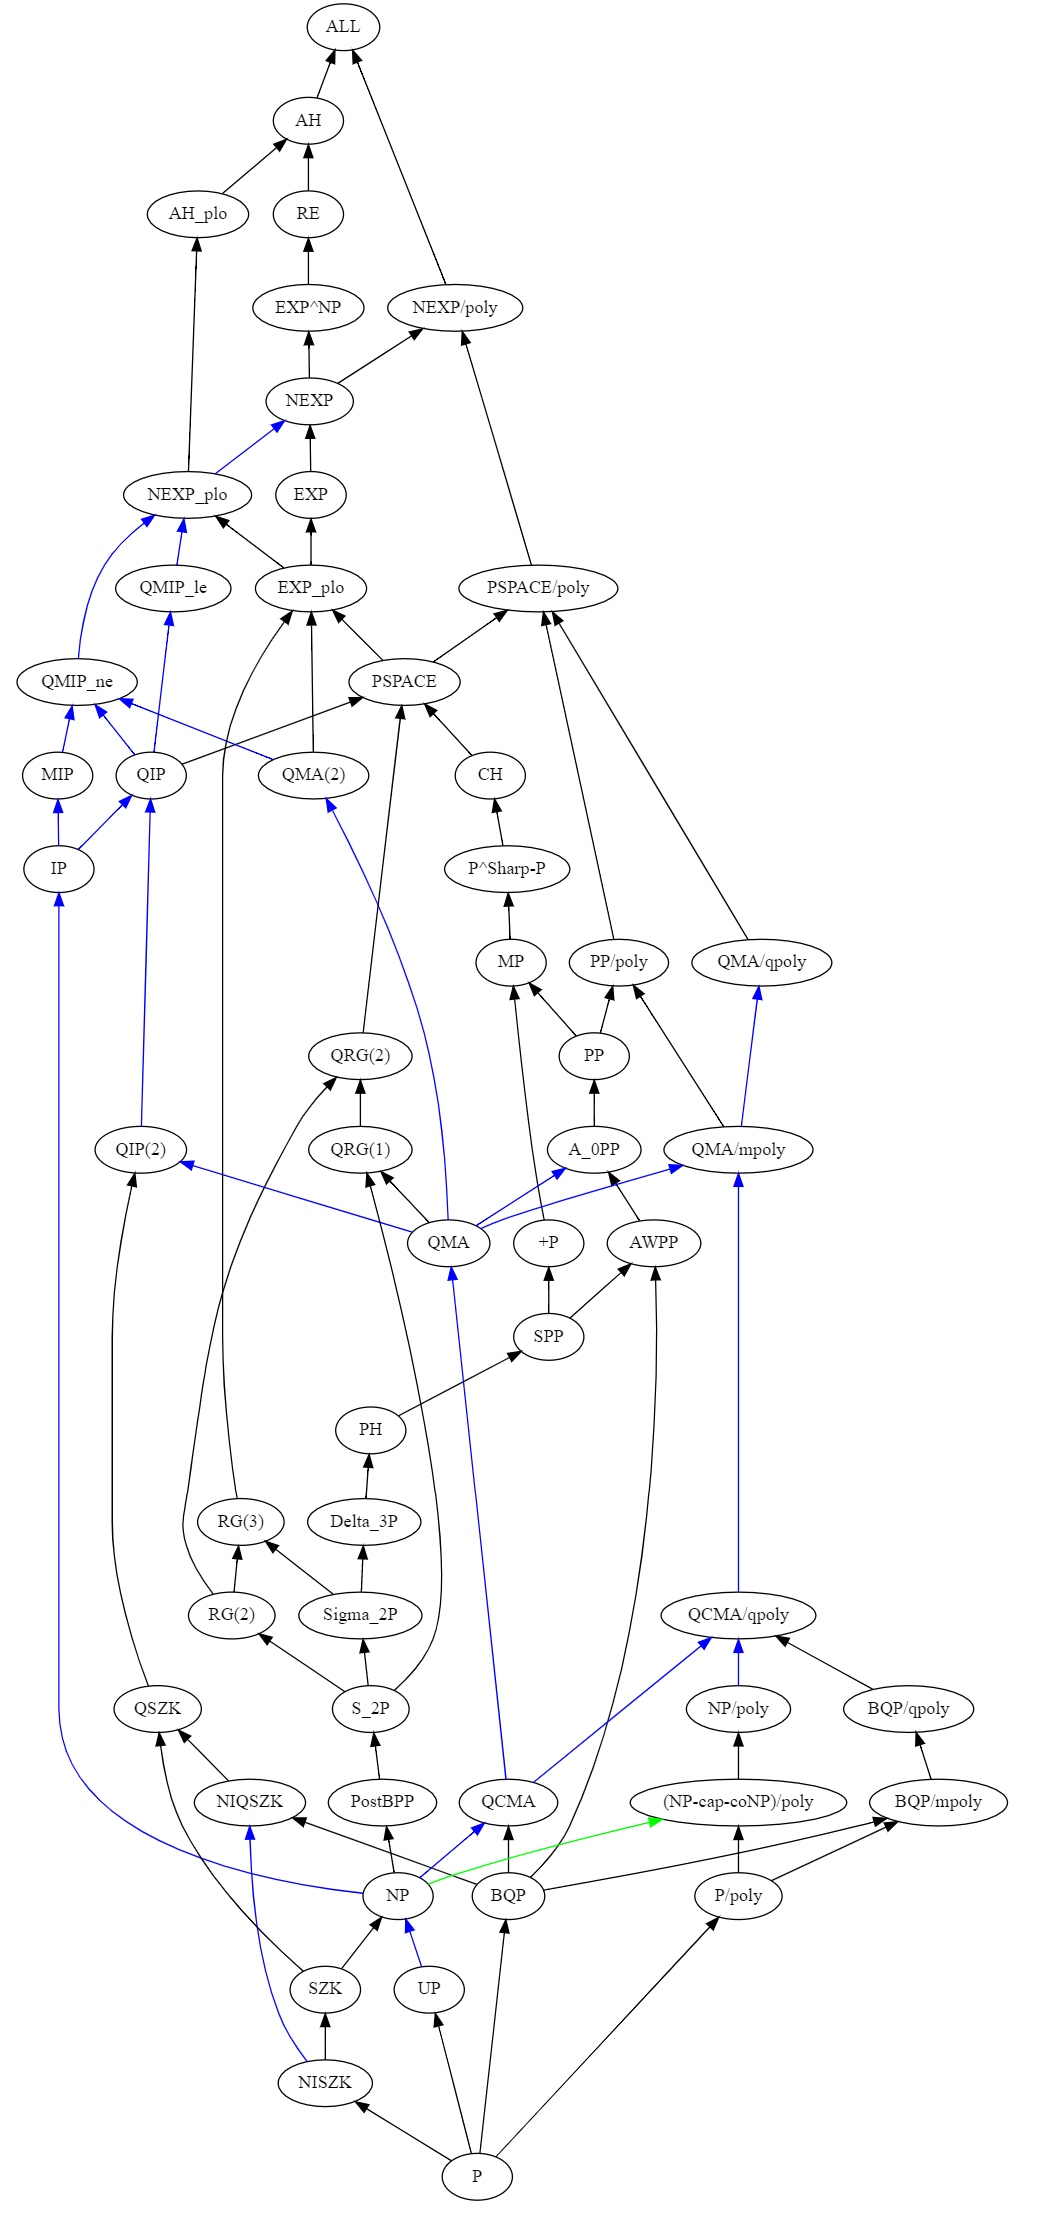
\includegraphics[height=8in]
  {random-oracle-full.png}}
  \caption{\label{fig:mini-zoo-inclusion} Inclusions that hold with respect to 
  the random oracle.}
\end{figure}

\begin{figure}[htb]
  \center{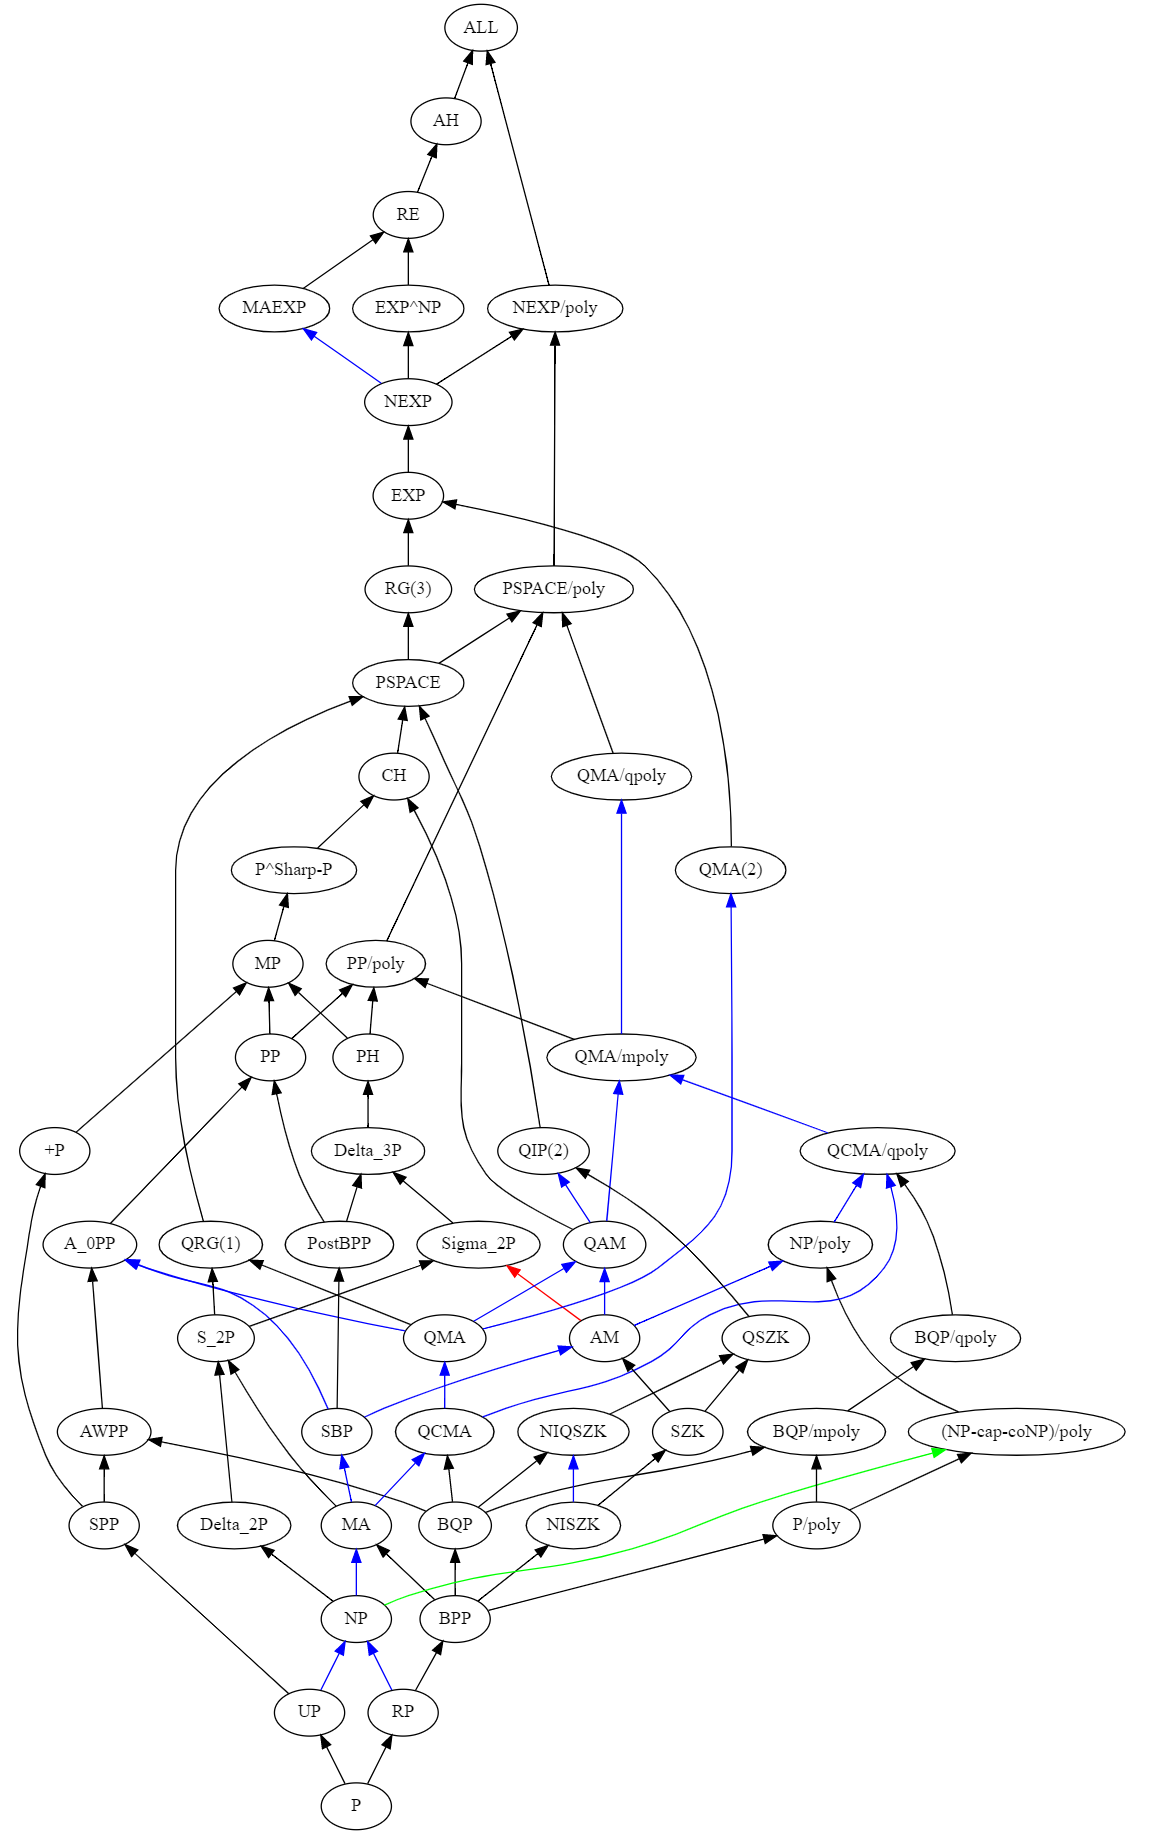
\includegraphics[height=8in]
  {trivial-oracle-full.png}}
  \caption{\label{fig:mini-zoo-inclusion} Inclusions that hold with respect to 
  the trivial oracle (the unrelativized world).}
\end{figure}

\subsection{$\oplus\msf{P}$}

$\oplus\sP$ is the class of languages $\cL$ such that for an $\NP$-machine
$M$ $x\in\cL$ if and only if the computational tree of $M(x)$ has an odd number
of accepting paths. In operator terms, it is equal to $\oplus\cdot\sP$.

$\oplus\sP\subseteq\msf{MP}$ with respect to every oracle \cite{green1995power}.
$\oplus\sP\not\subseteq\msf{PP}/\poly$ with respect to the random oracle, while 
it is open whether this is the case with respect to the trivial oracle.

\subsection{$\msf{A}_0\msf{PP}$}

A function $f:\Sigma^*\ra\Z$ lies in $\msf{GapP}$ if and only if there
exists a polynomial-time Turing machine $M$ and a function $p(n)=\Oh(n^*)$ such 
that for every $x\in\Sigma^*$,
\[
f(x)=|\{y\in\Sigma^{p(|x|)}:M(x,y)=1\}|-|\{y\in\Sigma^{p(|x|)}:M(x,y)=0\}|.
\]
Now $\cL\in\msf{A}_0\msf{PP}$ if and only if there exists a function
$f\in\msf{GapP}$ and a function $g:\Sigma^*\ra\N$ in $\msf{FP}$ such that
\begin{align*}
x\in\cL&\Longrightarrow f(x)>g(x), \\
x\not\in\cL&\Longrightarrow f(x)<g(x)/2.
\end{align*}
Note that a language in $\cL\in\msf{PP}$ can be characterized by the sign of 
some $\msf{GapP}$ function. Since $\msf{GapP}$ is closed under subtraction, it 
follows that $\msf{A}_0\msf{PP}\subseteq\msf{PP}$ for all oracles.

Kuperberg has also shown \cite{kuperberg2009hard} that $\msf{A}_0\msf{PP}$ is equal
to the class $\msf{SBQP}$ of languages $\cL$ such that there exists a 
$\msf{BQP}$-machine $M$ and a function $p(n)=\Oh(n^*)$ such that for all 
$x\in\Sigma^*$,
\begin{align*}
x\in\cL&\Longrightarrow\Pr[M(x)=1]\geq 2^{-p(|x|)}, \\
x\not\in\cL&\Longrightarrow\Pr[M(x)=1]\leq 2^{-p(|x|)-1}.
\end{align*}

\subsection{$\msf{AH}$}

The \textit{arithmetical hierarchy} is analogous to the polynomial hierarchy,
except that $\msf{R}$ and $\msf{RE}$ are the fundamental complexity classes
rather than $\sP$ and $\NP$. Thus, where $\msf{PH}$ is a hierarchy of 
complexity, $\msf{AH}$ is one of computability. For every $n\in\N$, define 
$\Delta_n$, $\Sigma_n$, and $\Pi_n$ by recursion as
follows: $\Delta_0=\Sigma_0=\Pi_0=\msf{R}$, and for every $n\in\N$,
\begin{align*}
\Delta_{n+1}&=\msf{R}^{\Sigma_n}, \\
\Sigma_{n+1}&=\msf{RE}^{\Sigma_n}, \\
\Pi_{n+1}&=\cco\cdot\msf{RE}^{\Sigma_n}.
\end{align*}
Then set $\msf{AH}=\bigcup_{n\in\N}\Sigma_n$.

Since $\msf{R}\subseteq\msf{RE}$ and $\msf{R}$ is a symmetric class it is
immediate that $\Delta_n\subseteq\Sigma_n$ and $\Delta_n\subseteq\Pi_n$ for all
$n\in\N$. Moreover, for $n\geq 1$ we have
\[
\Sigma_n=\msf{RE}^{\Sigma_{n-1}}\subseteq\msf{R}^{\msf{RE}^{\Sigma_{n-1}}}
=\msf{R}^{\Sigma_n}=\Delta_{n+1},
\]
and for $n=0$ we have
\[
\Sigma_0=\msf{R}\subseteq\msf{R}^{\msf{R}}=R^{\Sigma_0}=\Delta_1,
\]
so we also have $\Sigma_n\subseteq\Delta_{n+1}$ and $\Pi_n\subseteq\Delta_{n+1}$
for all $n\in\N$. It follows that
$\msf{AH}=\bigcup_{n\in\N}\Delta_n=\bigcup_{n\in\N}\Pi_n$. Also, just as there 
is an alternating quantifier definition for the polynomial hierarchy, there is 
one for the arithmetical hierarchy. For example, $\cL\in\Sigma_2$ if and only 
there exists a computable relation $R$ such that
\[
x\in\cL\Longleftrightarrow (\exists y)(\forall z)R(x,y,z)
\]
for each $x\in\Sigma^*$.

$\msf{AH}$ is closed under exponential padding: $\msf{AH}=\exppad\cdot\msf{AH}$.

\subsection{$\msf{AH}_{plo}$}\label{ah-plo-subsection}

$\msf{AH}_{plo}$ denotes $\msf{AH}$ with a polynomially-limited oracle
access. The definitions of $\msf{AH}_{plo}$ and $\msf{AH}$ in the
unrelativized case are identical, but $\msf{AH}^f$ and $\msf{AH}_{plo}^f$
have different definitions for an arbitrary oracle $f$.

For $n\in\N$ and an oracle $f:\Sigma^*\ra\Sigma^*$, we define 
$f|_n:\Sigma^*\ra\Sigma^*$ according to the
rule
\[
f|_n(x)=\begin{cases}f(x) &\text{ if }|x|<n, \\
0 &\text{ otherwise}.\end{cases}
\]
then we say that $\cL$ lies in $\msf{RE}_{\msf{plo}}^f$ if and only if there exists an oracle Turing machine $M$ and a function $p(n)=\Oh(n^*)$ such that
\[
x\in\cL\Longrightarrow M\text{ accepts }x\text{ with
}f|_{p(|x|)}\text{-oracle}.
\]
Now we can define $\msf{AH}_{plo}^f$ as we defined $\msf{AH}$: use 
$\msf{RE}_{plo}^f$ and $\msf{R}_{plo}^f=\cocap\cdot\msf{RE}_{plo}^f$ in the 
place of $\msf{RE}$ and $\msf{R}$ in the unrelativized definition of $\msf{AH}$.

$\msf{AH}_{plo}$ is not contained in $\msf{NEXP}/\poly$ and $\msf{RE}$ with 
respect to the random oracle.

Limiting $\msf{AH}$ to polynomial-length oracle queries has the effect of
creating an oracle collapse from $\msf{AH}$ all the way to $\sP$. In fact, we
can prove something even stronger: there exists an oracle relative to which
$\sP=\msf{AH}[poly]$, where $\msf{AH}[poly]$ is a class containing
$\msf{AH}$. 
$\msf{AH}[poly]$ is the class of languages $\cL$ such that there exists a
computable relation $R$ and a function $p(n)=\Oh(n^*)$ such that for every
$x\in\Sigma^*$,
\begin{align*}
x\in\cL\Longleftrightarrow
&(Q_1y_1\in\Sigma^*)\ldots(Q_{p(|x|)}y_{p(|x|)}\in\Sigma^*)
R(x,y_1,\ldots,y_{p(|x|)})\hspace{6pt}\OR \\
&(\bar Q_1y_1\in\Sigma^*)\ldots(\bar Q_{p(|x|)}y_{p(|x|)}\in\Sigma^*)
R(x,y_1,\ldots,y_{p(|x|)}),
\end{align*}
where $Q_k$ is $\forall$ when $k$ is even and $\exists$ when $k$ is odd, and
$\bar Q_k$ is $\exists$ when $k$ is even and $\forall$ when $k$ is odd.

The relativizing inclusion $\msf{AH}\subseteq\msf{AH}[poly]$ is immediate from
the alternating quantifier definition of $\msf{AH}$. Using the same quantifier definition as above, set
\begin{align*}
\mathtt{AHSAT}=&\{\inner{\alpha,x,1^m}:
(Q_1y_1\in\Sigma^*)\ldots(Q_my_m\in\Sigma^*)[M_\alpha(x,y_1,\ldots,y_m)=1])
\text{ or }\\
&(\bar Q_1y_1\in\Sigma^*)\ldots(\bar Q_my_m)\in\Sigma^*)
[M_\alpha(x,y_1,\ldots,y_m)=1])\},
\end{align*}
where $M_\alpha$ denotes the Turing machine that $\alpha$ encodes.
\begin{proposition}
$\mathtt{AHSAT}$ is $\msf{AH}[poly]$-complete.
\end{proposition}
\begin{proof}
To see that $\mathtt{AHSAT}\in\msf{AH}[poly]$, we can simply take $p$ to be the
identity function and $R$ to be the relation
\[
R(\inner{\alpha,x,1^m},y_1,\ldots,y_r)\Longleftrightarrow
r\geq m\AND M_\alpha(x,y_1,\ldots,y_m)=1.
\]
Then $R$ and $p$ witness that $\mathtt{AHSAT}\in\msf{AH}[poly]$ per the
definition.

Now suppose that $\cL\in\msf{AH}[poly]$, and let the relation $R$ and the
function $p(n)=\Oh(n^*)$ witness that $\cL\in\msf{AH}[poly]$. Then, if $\alpha$ is
a code for the Turing machine that computes $R$, we have
\[
x\in\cL\Longleftrightarrow\inner{\alpha,x,1^{p(|x|)}}\in\mathtt{AHSAT}.
\]
Since $p$ is assumed to be time-constructible, the function
$x\mapsto\inner{\alpha,x,1^{p(|x|)}}$ is polynomial-time computable, and so
$\cL$ is polynomial-time reducible to $\mathtt{AHSAT}$. Therefore,
$\mathtt{AHSAT}$ is a complete problem for $\msf{AH}[poly]$.
\end{proof}
Since $\sP\subseteq\msf{AH}[poly]$ relative to any oracle, in particular
$\sP^{\mathtt{AHSAT}}\subseteq\msf{AH}[poly]_{plo}^{\mathtt{AHSAT}}$. Moreover, 
adding an oracle for a problem in $\msf{AH}[poly]$ does not
increase the computational power of $\msf{AH}[poly]_{plo}$, because oracle calls
can be replaced with references to the alternating-quantifier relation 
corresponding to the oracle. So
$\msf{AH}[poly]_{plo}^{\mathtt{AHSAT}}\subseteq\msf{AH}[poly]\subseteq
\sP^{\mathtt{AHSAT}}$. Hence:
\begin{theorem}[Kuperberg]
$\sP^{\mathtt{AHSAT}}=\msf{AH}[poly]_{plo}^{\mathtt{AHSAT}}$.
\end{theorem}

\subsection{$\msf{ALL}$}

$\msf{ALL}$ is the ``complexity'' class of all languages.

While it is not an interesting complexity class in and of itself, $\msf{ALL}$ is
a useful point of reference in the hierarchy of complexity class inclusions. For
instance, it can be helpful to know which classes are immediately below
$\msf{ALL}$ in out hierarchy of inclusions, and it is often a nontrivial theorem
that a particular class is or is not $\msf{ALL}$.

\subsection{$\msf{AM}$}

$\msf{AM}$ is the class of language that can be computed using the
\textit{Arthur-Merlin protocol}. The protocol consists of these steps:
\begin{enumerate}
\item Arthur queries Merlin in an attempt to determine whether $x\in\cL$. Arthur
  is a polynomial-time Turing machine with access to a polynomial-length,
  uniformly random string $y$ of bits. This string is sent to Merlin.
\item Merlin sends a purported proof $z$ (with $|z|$ a polynomial of the length of
  the input) that $x\in\cL$. Merlin is an oracle with access to Arthur's coin 
  tosses, so Merlin can send any $z$ based on the situation.
\item Arthur decides whether to accept the input $x$ based on $\inner{x,y,z}$.
\end{enumerate}
The language $\cL$ is considered to lie in $\msf{AM}$ if the Arthur-Merlin
protocol is likely decide the question of whether $x\in\cL$ correctly. Formally,
we can set $\msf{AM}=\cBP\cdot\msf{NP}$.

Immediately, $\msf{AM}$ is contained in $\msf{QAM}$, $\msf{IP}$, and 
$\msf{RG}(2)$ for every oracle. It is also the case that 
$\msf{AM}\subseteq\Pi_2\sP$ for every oracle \cite{babai1985trading}. On the 
other hand, there is an oracle relative to which $\msf{AM}\not\subseteq\msf{PP}$
\cite{vereschchagin1992power}, and $\msf{AM}\subseteq\msf{NP}$ with respect to 
the random oracle \cite{babai1988arthur}.

\subsection{$\msf{AP}$}

An \textit{alternating Turing machine} is a non-deterministic Turing machine in
which each state is assigned either the symbol $\wedge$ or the symbol
$\vee$. Each configuration in a computational tree involving an alternating
Turing machine can likewise be assigned $\wedge$ or $\vee$ based on the current
state of the machine.

To determine whether an alternating Turing machine $M$ accepts an input $x$,
assign an element of $\Sigma$ to each node in the computational tree according
to the following procedure:
\begin{enumerate}
\item If a configuration $c$ is a halting configuration, set $v(c)=0$ if the
  output is 0 and $v(c)=1$ if the output is 1.
\item If $c$ is an $\wedge$-configuration, assign $v(c)=1$ if $v(c^\prime)=1$
  for each descendant $c^\prime$ of $c$ in the computational tree. Otherwise,
  set $v(c)=0$.
\item If $c$ is an $\vee$-configuration, assign $v(c)=1$ if $v(c^\prime)=1$ for
  some descendant $c^\prime$ of $c$ in the computational tree.
\end{enumerate}
Then, we say that $M$ accepts the input $x$ if and only if
$v(s_{\text{start}})=1$.

$\cL\in\msf{AP}$ if there exists a polynomial-time alternating Turing machine
$M$ such that
\[
x\in\cL\Longleftrightarrow M\text{ accepts }x.
\]
for every $x\in\Sigma^*$.

$\msf{AP}=\msf{PSPACE}$ for every oracle \cite{chandra1981alternation}.

\subsection{$\msf{AWPP}$}

$\msf{AWPP}$ is the class of ``almost wide'' $\msf{PP}$ problems. For a 
polynomial-time Turing machine $M$ and a function $p(n)=\Oh(n^*)$, define
\[
d_{M,p}(x)=|\{y\in\Sigma^{p(|x|)}:M(x,y)=0\}|-|\{y\in\Sigma^{p(|x|)}:M(x,y)=1\}|
\]
for each $x\in\Sigma^*$. $\cL\in\msf{AWPP}$ if there exists a polynomial-time 
Turing machine $M$, a function $f:\Sigma^*\ra\N$, and functions 
$p(n),q(n)=\Oh(n^*)$ such that
\begin{align*}
x\in\cL&\Longrightarrow(1-2^{-q(|x|)})f(x)\leq d_{M,p}(x)\leq f(x), \\
x\not\in\cL&\Longrightarrow 0\leq d_{M,p}(x)\leq 2^{-q(|x|)}f(x).
\end{align*}
$\msf{AWPP}\subseteq\msf{A}_0\msf{PP}$ for all oracles \cite{vyalyi2003qma}.

\subsection{$\msf{BPP}$}

This is the class of languages computable in polynomial time using randomness, 
where the computer is correct with a probability of at least $2/3$. In other 
words, $\msf{BPP}=\cBP\cdot\sP$.

It is contained in $\msf{BQP}$, $\msf{MA}$, $\msf{NISZK}$,  and $\msf{SZK}$ with
respect to every oracle. $\msf{BPP}\subseteq\Sigma_2$ for every oracle 
\cite{lautemann1983bpp}, but there is an oracle relative to which 
$\msf{BPP}\not\subseteq\Delta_2\sP$. In the random oracle world, $\sP=\msf{BPP}$
\cite{bennett1981relative}. $\msf{BPP}\not\subseteq\Delta_2\sP$ is open in the 
unrelativized world.

\subsection{$\msf{BPP}_{path}$}

$\msf{BPP}_{path}$ is the original name for $\msf{PostBPP}$, or $\msf{BPP}$ with 
postselection. It was originally defined as the class of all languages $\cL$ such 
that there exists a non-deterministic polynomial-time Turing machine $M$ and a 
threshold $\epsilon>0$ such that for every $x\in\Sigma^*$, the number of paths for
which $M(x)=\cL(x)$ is at least $(1/2+\epsilon)\cdot T(x)$, where $T(x)$ is the 
total number of computational paths of $M$ with input $x$  
\cite{han1997threshold}.

\subsection{$\msf{BQP}$}

Informally, $\msf{BQP}$ is the set of languages that can be computed efficiently
using a quantum computer. A quantum computer can be modeled by a uniform family 
of quantum circuits or a quantum Turing machines whose configurations can be 
quantum states.

$\msf{BQP}\subseteq\msf{BQP}/\msf{mpoly}$ is immediate. $\msf{BQP}$ is also 
contained in $\msf{AWPP}$ for every oracle \cite{fortnow1998complexity}, as well
as $\msf{NIQSZK}$, $\msf{QCMA}$, and $\msf{QSZK}$. There exist oracles relative 
to which $\msf{BQP}$ is not contained in $\oplus\sP$, $\msf{PH}$, $\msf{MA}$ 
\cite{watrous2000succinct}, $\NP/\poly$, $\msf{PostBPP}$ \cite{aaronson2010bqp} 
\cite{chen2016note},
and $\msf{SZK}$ \cite{childs2003exponential}. Recently, $\msf{PH}$ was added to 
this list of oracle separations \cite{raz2018oracle}.

In the random oracle world, the following inclusions are open:
\[
\msf{BQP}\subseteq\msf{BPP},\msf{IP},\msf{MIP},\sP,\msf{PH},\oplus\sP,\NP/\poly.
\]
It is also open whether $\msf{BQP}$ is contained in $\msf{PH}$ and $\NP/\poly$ 
in the unrelativized world and whether there exists an oracle such that 
$\msf{BQP}\not\subseteq\msf{MIP}$.

\subsection{$\msf{BQP}/\msf{mpoly}$}\label{bqp-mpoly}

$\msf{BQP}/\msf{mpoly}$ is $\msf{BQP}$ with ``Merlinized'' polynomial advice.
\begin{definition}
$\cL\in\msf{BQP}/\msf{mpoly}$ if there exists a $\msf{BQP}$-machine $M$ and a
polynomial-length advice function $f:\N\ra\Sigma^*$ such that
\[
x\in\cL\Longleftrightarrow\Pr[M(x,f(n))=\cL(x)]\geq 2/3.
\]
\end{definition}
The advice is ``Merlinized'' in the sense that the probability threshold of $\geq 
2/3$ need only be observed when the advice is good, just as Arthur does not need 
to satisfy the probability gap when Merlin gives a poor argument in the 
Arthur-Merlin protocol.

$\msf{BQP}/\msf{mpoly}$ is also the class of languages that can be computed using 
some family of polynomial-sized quantum circuits.

$\msf{BQP}/\msf{mpoly}\subseteq\msf{BQP}/\msf{qpoly},\msf{QMA}/\msf{qpoly}$ for 
every oracle.

\subsection{$\msf{BQP}/\msf{qpoly}$}

$\msf{BQP}/\msf{qpoly}$ is $\msf{BQP}$ with a polynomial amount of quantum 
advice. This means that, rather than a classical advice string, a 
$\msf{BQP}$-machine is given an advice string that 
exists in a state of superposition. That is, the advice string takes the form 
$\sum_s\alpha_s\ket{s}$, where the sum is over polynomial-length strings in 
$\Sigma$.

It is immediate that $\msf{BQP}/\msf{qpoly}\subseteq\msf{QCMA}/\msf{qpoly}$ 
relative to every oracle. In fact, Aaronson and Drucker have shown that 
$\msf{BQP}/\msf{qpoly}\subseteq\msf{QCMA}/\msf{mpoly}$ 
\cite{aaronson2010characterization}. The relationship between classical and quantum
advice in the case of $\msf{BQP}$ is uncertain: it is unknown whether 
$\msf{BQP}/\msf{qpoly}$ is any larger than $\msf{BQP}/\msf{mpoly}$ 
\cite{aaronson2007quantum}.

\subsection{$\msf{BQPSPACE}$}

This is the class of languages computable by a \textit{quantum Turing machine} 
using a polynomial amount of space. A quantum Turing machine is a Turing machine 
that includes a quantum tape on which qubits can be recorded, as well as a finite 
register for performing measurements. As with other non-deterministic versions of 
$\msf{PSPACE}$ (see Subsections \ref{npspace-subsection} and 
\ref{ppspace-subsection}), $\msf{BQPSPACE}$ is equal to $\msf{PSPACE}$ for every 
oracle \cite{watrous2003complexity}.

\subsection{$\msf{CH}$}

The \textit{counting hierarchy} is the class that results from an infinite stack
of $\msf{PP}$-oracles. If $C_0\sP=\sP$ and $C_{k+1}\sP=\msf{PP}^{C_k\sP}$ for 
each $k\in\N$, then $\msf{CH}=\bigcup_kC_k\sP$. The classes $\sP^{C_k\sP}$ are 
clearly inside $\msf{CH}$, and so $\msf{CH}=\sP^{\msf{CH}}$ for every oracle. 
Moreover, because $\msf{PP}\subseteq\msf{PSPACE}$, and because giving 
$\msf{PSPACE}$ access to an oracle that is already inside $\msf{PSPACE}$ does 
not increase the power of the class, we also have the relativizing inclusion 
$\msf{CH}\subseteq\msf{PSPACE}$.

It is unknown whether $\msf{CH}\subseteq\sP^{\#\sP}$ (since 
$\sP^{\#\sP}=\sP^{\msf{PP}}$, this would imply that the counting hierarchy 
collapses) relative to a random oracle, and indeed whether there is any oracle 
relative to which the counting hierarchy does not collapse.

\subsection{$\cocap\cdot\msf{RE}$}

The class $\cocap\cdot\msf{RE}=\msf{RE}\cap\co\msf{RE}$ is equal to $\msf{R}$, 
the class of recursive decision problems. $\msf{RE}$ is the class of languages 
that a computer can enumerate the elements of. If a computer can enumerate the 
elements of a language as well as its complement, then the computer can decide 
whether $x$ lies in the language by enumerating the language and its complement 
until it is revealed where $x$ lies.

\subsection{$\cocap\cdot\msf{RP}$}

The intersection of $\msf{RP}$ and $\co\msf{RP}$ is equal to $\msf{ZPP}$ for 
every oracle.

\subsection{$\Delta_2\sP$}

The class $\Delta_2\sP$ is a level of the polynomial hierarchy, defined to be 
$\sP^\NP$. It is therefore contained in $\Sigma_2\sP=\NP^{\NP}$. Less obviously,
$\Delta_2\sP$ lies in $S_2\sP$ relative to every oracle 
\cite{russell1998symmetric}. While it is unknown whether 
$\Delta_2\sP\subseteq\msf{PP}$ in the unrelativized world, there exists an 
algebraic oracle relative to which $\Delta_2\sP\subseteq\msf{PP}$ 
\cite{aaronson2009algebrization}. $\Delta_2\sP$ is outside $\msf{PostBPP}$ 
relative to the random oracle.

\subsection{$\Delta_3\sP$}

This class is $\sP^{\Sigma_2\sP}$, another level of the polynomial hierarchy. It
is unknown whether $\Delta_3\sP\subseteq\msf{PostBPP}$ relative to the trivial 
oracle.

\subsection{$\msf{EXP}$}

This is the class of languages that can be decided in exponential time. It can 
be succinctly defined as $\exppad\cdot\sP$. By the time hierarchy theorem, 
$\msf{EXP}\not\subseteq\sP$ relative to every oracle, but there is an oracle 
relative to which $\msf{EXP}=\msf{ZPP}$ \cite{Heller1984}, as well as an oracle 
relative to which $\msf{EXP}=\cocap\cdot\msf{UP}$. In the unrelativized world, 
it is unknown whether either of these equalities is true.

\subsection{$\msf{EXP}^\NP$}

This class is $\bigcup_{f\in\NP}\msf{EXP}^f$, or $\msf{EXP}$ relative to an 
$\msf{NP}$-oracle. (It can also be defined to be $\msf{EXP}^{\mathtt{SAT}}$, or 
any other $\NP$-complete problem.) Since $\msf{EXP}=\exppad\cdot\sP$, it follows
that $\msf{EXP}^\NP=\exppad\cdot\Delta_2\sP$. There exist oracles relative to 
which this class is equal to $\msf{BPP}$ \cite{buhrman2000randomness} and 
$\msf{SPP}$. The time hierarchy theorem relativizes, so 
$\msf{EXP}^\NP\not\subseteq\Delta_2\sP$ for every oracle. Additionally, 
$\msf{EXP}^\NP\not\subseteq\msf{NEXP}$ in the random oracle world.

In the unrelativized world, the inclusions 
$\msf{EXP}^\NP\subseteq\msf{NEXP}/\poly,\msf{BPP},\msf{SPP}$ are open.

\subsection{$\msf{EXP}_{plo}$}

As with $\msf{AH}_{plo}$, $\msf{EXP}_{plo}$ is equal to $\msf{EXP}$ in the 
unrelativized world, while relative to an oracle, the oracle calls are limited 
in length to a polynomial of $|x|$ for the input $x$.

\subsection{$\msf{IP}$}

An \textit{interactive proof protocol} is an interaction between a probabilistic
polynomial-time verifier and a deterministic prover with infinite computational 
power. The prover can compute any function, but unlike the Arthur-Merlin 
protocol, the prover does not know the random bits that the verifier uses in his
computations. The verifier attempts to determine whether the input $x$ lies in a
given language $\cL$ within a number of rounds that is a polynomial of $|x|$. 
The language lies in $\msf{IP}$ if and only if the protocol is 
\textit{complete}, meaning that if $x\in\cL$ then the verifier can be convinced 
of this fact with a probability of at least $2/3$, and \textit{sound}, meaning 
that if $x\not\in\cL$ then the verifier can be convinced that $x\in\cL$ with a 
probability of at most $1/3$.

While the prover has the power to determine even uncomputable functions, to 
determine the optimal strategy for the prover, given an input $x$, only a 
$\msf{PSPACE}$-machine is necessary. Using a polynomial-space computation, the 
prover can simulate as many interactions with the prover as needed. Therefore, 
$\msf{IP}\subseteq\msf{PSPACE}$ relative to every oracle.

$\msf{IP}$ is also contained in its generalizations $\msf{QIP}$ and $\msf{MIP}$.
There is an oracle relative to which $\cocap\cdot\msf{IP}\not\subseteq\msf{PH}$ 
\cite{aiello1990power}. Open problems in the random oracle world include whether
$\cocap\cdot\msf{IP}$ is contained in $\msf{PP}/\poly$, $\msf{QMA}/\msf{qpoly}$,
$\msf{CH}$, or $\msf{QMA}(2)$.

\subsection{$\msf{IPP}$}

This class is the unbounded version of $\msf{IP}$. More precisely, the 
completeness and soundness conditions are weakened so that when $x\in\cL$, the 
prover can convince the verifier to accept with a probability of at least $1/2$,
while if $x\not\in\cL$, then in all circumstances the verifier accepts with a 
probability of at most $1/2$. $\msf{IPP}=\msf{PSPACE}$ with respect to every 
oracle \cite{chang1994random}.

\subsection{$\msf{MA}$}

The Merlin-Arthur protocol is similar to the Arthur-Merlin protocol, except that
Merlin sends Arthur a message without knowing Arthur's randomized bits, and 
Arthur decides whether to accept that the input $x$ lies in the language $\cL$ 
using a polynomial-time randomized algorithm. As with many other interaction 
protocols, $\cL\in\msf{MA}$ if and only only if $x\in\cL$ implies that Arthur 
can be persuaded that $x\in\cL$ with probability $\geq 2/3$, while $x\not\in\cL$
implies that Arthur can be persuaded that $x\in\cL$ with probability $\leq 2/3$.

$\msf{MA}\subseteq\msf{QCMA},\msf{SBP}$ relative to every oracle. It is also the
case that $\msf{MA}\subseteq\msf{S}_2\sP$ relative to every oracle 
\cite{russell1998symmetric}. In the unrelativized world, the inclusion 
$\cocap\cdot\msf{MA}\subseteq(\NP\cap\co\NP)/\poly$ is open.

\subsection{$\msf{MAEXP}$}

The class $\msf{MAEXP}$ is the class of languages computable using the 
Merlin-Arthur protocol, where Arthur has exponential computational power. In 
operator terms, $\msf{MAEXP}=\exppad\cdot\msf{MA}$. $\msf{MA}$ is strictly 
contained in $\msf{MAEXP}$ relative to every oracle.

There exist oracles relative to which $\msf{MAEXP}$ is contained in $\oplus\sP$,
$\Delta_2\sP$, and $\sP/\poly$, while in the unrelativized world, 
$\cocap\cdot\msf{MAEXP}\not\subseteq\sP/\poly$ 
\cite{buhrman1998nonrelativizing}. In fact, 
$\cocap\cdot\msf{MAEXP}\not\subseteq\sP/\poly$ relative to every algebraic 
oracle \cite{aaronson2009algebrization}. Relative to the trivial oracle, it is 
open whether $\msf{MAEXP}$ is contained in $(\NP\cap\co\NP)/\poly$, $\msf{BQP}$,
$\Delta_2\sP$, $\msf{SPP}$, $\cocap\cdot\msf{NISZK}$, or $\cocap\cdot\msf{SBP}$.

\subsection{$\msf{MIP}$}

An interactive proof protocol can involve multiple provers. In the class 
$\msf{MIP}$, there are two provers and one verifier. As in $\msf{IP}$, the 
verifier is a polynomial-time probabilistic Turing machine and the provers have 
infinite computing power; however, the provers are not allowed to communicate 
with each other.

$\msf{MIP}$ is contained in $\msf{NEXP}_{plo}$ and its quantum counterpart 
$\msf{QMIP}_{ne}$ relative to every oracle. Open questions include whether  
$\msf{MIP}\subseteq\cco\cdot\msf{MAEXP}$ for every oracle, whether 
$\msf{MIP}\subseteq\cco\cdot\msf{NEXP}$ for the random oracle, and whether 
$\cocap\cdot\msf{MIP}\subseteq\msf{EXP}$ for all oracles and for the random 
oracle.

\subsection{$\msf{MP}$}

For $x\in\Sigma^*$, denote by $x(k)\in\Sigma$ the bit in $x$ at position $k$ 
(indexing from zero). Then, we say $\cL\in\msf{MP}$ if and only if there exists 
$f\in\#\sP$ and a polynomial-time computable $g:\Sigma^*\ra\N$ such that 
$\cL(x)=f(x)(g(x))$ for every $x\in\Sigma^*$. $\msf{MP}$ stands for ``middle 
bit,'' because it can be assumed that $|f(x)|$ is always odd and that 
$g(x)=\frac{1}{2}(|f(x)|-1)$ \cite{green1995power}.

$\msf{MP}$ is contained in $\sP^{\#\sP}$ relative to every oracle, since 
$\sP^{\#\sP}$ can use a $\#\sP$-oracle to determine the middle bit of a function
in $\#\sP$.

\subsection{$\msf{NEXP}$}

This class is the non-deterministic counterpart to $\msf{EXP}$; it can be 
defined to be $\exppad\cdot\NP$. Like $\NP$, it is distinct from its complement 
with respect to an oracle constructed via the password argument. Additionally, 
$\cocap\cdot\msf{NEXP}\not\subseteq\NP$ with respect to every oracle by a 
diagonalization argument.

There exists an oracle relative to which $\msf{NEXP}\subseteq\oplus\sP$ 
\cite{aaronson2006oracles}. In the unrelativized world, the inclusions 
$\msf{NEXP}\subseteq\msf{SPP}$ and $\msf{NEXP}\subseteq\cco\cdot\msf{MAEXP}$ are 
open.

\subsection{$\msf{NEXP}_{plo}$}

This class is identical to $\msf{NEXP}$, except that oracle calls are limited in
length to a polynomial of $|x|$ for input $x$. It is contained in $\msf{MIP}$ 
\cite{aaronson2009algebrization} and $\msf{QMIP}_{le}$ \cite{ito2012multi} with 
respect to all algebraic oracles. The question of whether 
$\msf{NEXP}_{plo}\subseteq\msf{MP}$ relative to every oracle is open.

\subsection{$\msf{NEXP}/\poly$}

Naturally, $\msf{NEXP}/\poly$ is defined to be $\cpoly\cdot\msf{NEXP}$. The 
question of whether $\msf{NEXP}/\poly\subseteq\sP/\poly$ in the unrelativized 
world is open.

\subsection{$\msf{NIQSZK}$}

This class is the non-interactive version of $\msf{QSZK}$, just as $\msf{NISZK}$
is the non-interactive version of $\msf{SZK}$. Accordingly, it lies in 
$\msf{QSZK}$ for every oracle. The inclusions 
\[
\cocap\cdot\msf{NIQSZK}\subseteq\msf{CH},\msf{PP}/\poly,\msf{QMA}/\msf{qpoly}
\]
are open with respect to the trivial oracle.

\subsection{$\msf{NISZK}$}
There is a modified version of the statistical zero-knowledge protocol in which 
interaction between the prover and the verifier is disallowed. More precisely, a
language lies in $\msf{NISZK}$ if and only if the language can be computed using
a statistical zero-knowledge protocol, with the additional constraints that the 
prover and verifier share a single randomly generated string as the source of 
their randomness, and the only communication allowed between the two parties is 
a single message from the prover to the verifier.

There exist oracles relative to which 
$\cocap\cdot\msf{NISZK}\not\subseteq\msf{PP}$ \cite{bouland2017power} and 
$\cocap\cdot\msf{NISZK}\not\subseteq\msf{BQP}/\msf{qpoly}$. Unlike $\msf{SZK}$, 
there is an oracle which $\msf{NISZK}$ is distinct from its complement 
\cite{lovett2017impossibility}. It is open whether 
$\msf{NISZK}\subseteq\msf{NIQSZK}$ in either the world of all oracles or in the 
unrelativized world. The inclusions
\[
\cocap\cdot\msf{NISZK}\subseteq\msf{BQP}/\msf{qpoly},\msf{PP},\msf{QMA}(2),
\msf{QRG}(1),(\NP\cap\co\NP)/\poly
\]
are likewise open in the unrelativized world.

\subsection{$\NP$}

The class of languages that can be computed in non-deterministic polynomial time
can, naturally, be defined to be $\cN\cdot\sP$. It is immediate that 
$\NP\subseteq\msf{MA}$ for every oracle, since $\NP$ is precisely the result of 
the Merlin-Arthur protocol with a deterministic Arthur. Put another way, $\NP$ 
is the class of languages $\cL$ such that if $x\in\cL$, then there is a proof of
this fact that a computer can check in time $p(|x|)$ for some $p(n)=\Oh(n^*)$.

As it is one of the most thoroughly studied complexity classes, there are many 
known oracle separations involving $\NP$. With respect to the random oracle, 
$\NP\not\subseteq\msf{UP}$ \cite{beigel1989relativized} and 
$\NP\not\subseteq\msf{BQP}$ \cite{bennett1997strengths}. There exist oracles 
relative to which $\NP\cap\co\NP\not\subseteq\msf{BQP}$ 
\cite{bennett1997strengths}, $\NP\not\subseteq\msf{BQP}/\msf{qpoly}$ 
\cite{aaronson2004limitations}, $\NP\not\subseteq\cco\cdot\msf{IP}$, 
$\NP\cap\co\NP\not\subseteq\msf{AWPP}$, 
$\NP\not\subseteq\cco\cdot\msf{A}_0\msf{PP}$, and there exist algebraic oracles 
relative to which $\NP\not\subseteq\msf{BQP}$ and 
$\NP\not\subseteq\cco\cdot\msf{MA}$ \cite{aaronson2009algebrization}.

In addition to the famous $\NP\subseteq\sP$ and $\NP\subseteq\co\NP$ in the 
unrelativized world, open questions include whether $\NP\cap\co\NP\subseteq\sP$ 
relative to the random oracle, whether $\NP\subseteq\cco\cdot\msf{A}_0\msf{PP}$ 
or $\NP\cap\co\NP\subseteq\msf{AWPP}$ relative to the trivial oracle, and 
whether $\NP\subseteq\cco\cdot\msf{AM}$ relative to every algebraic oracle.

\subsection{$(\NP\cap\co\NP)/\poly$}

As the class's name would suggest, 
$(\NP\cap\co\NP)/\poly=\cpoly\cdot\cocap\cdot\NP$. Complexity Zoology is able to 
determine the place of this class in the inclusion hierarchy automatically 
through the properties of complexity class operators. In the random oracle 
world, the inclusion $(\NP\cap\co\NP)/\poly\subseteq\sP/\poly$ is open.

\subsection{$\NP/\poly$}

Not only is $\NP/\poly=\cpoly\cdot\NP$, but by the same derandomization argument 
used to show $\msf{BPP}\subseteq\sP/\poly$, we also have 
$\NP/\poly=\cpoly\cdot\msf{AM}$.

Since $\NP\subseteq\msf{MA}$, it follows that 
$\NP/\poly\subseteq\msf{QMA}/\msf{mpoly}$ for every oracle. Likewise, 
$\NP/\poly\subseteq\msf{QCMA}/\msf{qpoly}$ for every oracle. On the other hand, 
there is an oracle relative to which 
$\NP/\poly\not\subseteq(\NP\cap\co\NP)/\poly$ \cite{fenner2003oracle}.

\subsection{$\msf{NPSPACE}$} \label{npspace-subsection}

This class is the non-deterministic version of $\msf{PSPACE}$: 
$\msf{NPSPACE}=\cN\cdot\msf{PSPACE}$. However, $\msf{NPSPACE}$ is no larger than
$\msf{PSPACE}$:
\begin{theorem}[Savitch, \cite{savitch1970relationships}]
$\msf{NPSPACE}=\msf{PSPACE}$ for every oracle.
\end{theorem}
\begin{proof}[Proof sketch]
Given a directed graph with a set $V$ of $n$ vertices and a pair of vertices 
$v,w$, write $\STCON(v,w,k)$ if there exists a path of length $\leq k$ connecting 
$v$ to $w$. To check whether $\STCON(v,w,k)$, recursively check whether each 
vertex $x$ lies halfway along a connecting path:
\[
\STCON(v,w,k)\Longleftrightarrow
\bigvee_{x\in V}(\STCON(v,x,\lfloor k/2\rfloor)\AND
\STCON(x,w,\lceil k/2\rceil))\hspace{12pt}(k\geq 2).
\]
The resulting algorithm uses an $\Oh((\log n)^2)$ amount of space.

Thus, given an $\Oh(f(n))$-space non-deterministic algorithm for a language $\cL$,
we check the $2^{\Oh(f(n))}$-vertex computational tree for a path from the 
starting configuration to the accepting configuration, resulting in a 
deterministic $\Oh((f(n))^2)$-space algorithm.
\end{proof}

\subsection{$\sP$}

The class of languages that are computable in polynomial time is the smallest 
class in Complexity Zoology's data set. There are smaller classes studied in 
complexity theory---such as $\msf{L}$, the class of languages that are 
computable using a logarithmic amount of space---$\sP$ is chosen as the bottom 
of the inclusion hierarchy so that, for instance, polynomial-length oracle calls
are allowed.

Since $\sP$ is the smallest class in Complexity Zoology's data set, it has 
relatively few relations in the input file: we have $\sP\subseteq\msf{UP}$ and 
$\sP\subseteq\msf{ZPP}$ relative to all oracles, both of which are immediate 
from the classes involved.

\subsection{$\sP/\poly$}

The class $\sP/\poly=\cpoly\cdot\sP$ is also equal to $\cpoly\cdot\sP$ is also 
equal to $\cpoly\cdot\msf{BPP}$ via the usual derandomization argument. 
$\sP/\poly\subseteq\msf{BQP}/\msf{mpoly}$ for every oracle, since the latter 
class is a generalization of $\sP/\poly$; and $\sP/\poly\not\subseteq\msf{AH}$ 
for every oracle, because $\sP/\poly$ is uncountable while $\msf{AH}$ is 
countable.

\subsection{$\sP^\msf{PP}$}

We have $\sP^{\msf{PP}}=\bigcup_{f\in\msf{PP}}\sP^f$. As was discussed in 
Section \ref{simplified-version}, $\sP^{\msf{PP}}=\sP^{\#\sP}$ for every oracle,
because we can simulate a $\#\sP$-oracle using multiple $\msf{PP}$-oracle calls.
We also have $\sP^{\msf{PP}}\subseteq\msf{PP}^{\msf{PP}}\subseteq\msf{PP}^{\msf{
C}_1\sP}\subseteq\msf{CH}$.

\subsection{$\sP^{\#\sP}$}

We have $\sP^{\#\sP}=\bigcup_{f\in\#\sP}\sP^f$. The inclusion 
$\sP^{\#\sP}\subseteq\msf{MP}$ is open for both the random and trivial oracles.

\subsection{$\msf{PH}$}

The \textit{polynomial hierarchy} is the class that results from an infinite 
hierarchy of $\NP$-oracles. We set $\Sigma_0\sP=\sP$ and 
$\Sigma_{k+1}\sP=\NP^{\Sigma_k\sP}$ for $k\in\N$, as well as 
$\Pi_k\sP=\cco\cdot\Sigma_k\sP$ and $\Delta_0\sP=\sP$, 
$\Delta_{k+1}\sP=P^{\Sigma_k\sP}$. $\msf{PH}$ is contained in $\msf{MP}$ 
\cite{green1995power} and $\msf{PP}/\poly$ with respect to every oracle, as well
as $\msf{SPP}$ with respect to the random oracle \cite{fortnow1999relativized}. 
On the other hand, $\msf{PH}\not\subseteq\Delta_3\sP$ with respect to the random
oracle, and the question of whether $\msf{PH}\subseteq\Delta_3\sP$ unrelativized
is open.

\subsection{$\msf{PostBPP}$}

The definition of this class is similar to that of $\msf{BPP}$, except we allow 
for \textit{postselection}. Let $(M,p)$ be a polynomial-time Turing machine and 
$\Oh(n^*)$-function, respectively,  such that
\[
\Pr_{y\in\Sigma^{p(|x|)}}[M(x,y)=1]>0
\]
for every $x\in\Sigma^*$. Then $\cL\in\msf{PostBPP}$ if and only if there exists
a polynomial-time Turing machine $M^\prime$ such that for all $x\in\Sigma^*$,
\[
\Pr_{y\in\Sigma^{p(|x|)}}[M^\prime(x,y)=\cL(x)|M(x,y)=1]\geq 2/3.
\]
The condition $M(x,y)=1$ effectively allows us to consider 
$\msf{BPP}$-algorithms in which there is an option for the program to 
\textit{quit} before concluding $x\in\cL$ or $x\not\in\cL$. The algorithm is 
considered successful if it has a high probability of reaching the correct 
answer when it does \textit{not} quit.

$\msf{PostBPP}$ is contained in $\Delta_2\sP$ with respect to the random oracle 
and $\Delta_3\sP$ and $\msf{PP}$ with respect to all oracles. The question of 
whether $\msf{PostBPP}\subseteq\Sigma_2\sP$ in the unrelativized world is open.

\subsection{$\msf{PostBQP}$}

This class is the quantum analogue of $\msf{PostBPP}$. For a $\msf{BQP}$-machine
$M$ and input $x$, denote the value of the $k$th qubit of the output by 
$M(x)_k$, $\cL\in\msf{PostBQP}$ if and only if there exists a 
$\msf{BQP}$-machine $M$ such that for every $x\in\Sigma^*$, $\Pr[M(x)_1=1]>0$ 
and
\[
\Pr[M(x)_0=\cL(x)|M(x)_1=1]\geq 2/3.
\]
It has been shown that $\msf{PostBQP}=\msf{PP}$ for every oracle 
\cite{aaronson2005quantum}.

\subsection{$\msf{PP}$}

Define $\msf{PP}$ to be $\cP\cdot\sP$. Like $\msf{BPP}$, $\msf{PP}$ is based on 
a probabilistic model of computation, except that the machine is only required 
to obtain the correct answer with a probability of at least $1/2$.

$\msf{PP}\subseteq\msf{MP}$ with respect to every oracle. Also, 
$\msf{PP}\subseteq\oplus\sP$ with respect to the random oracle \cite{Raz87b}.

\subsection{$\msf{PP}/\poly$}

This class is simply $\msf{PP}$ with polynomial advice: in operator terms, 
$\msf{PP}/\poly=\cpoly\cdot\cP\cdot\sP$.

\subsection{$\msf{PPSPACE}$} \label{ppspace-subsection}

This is a probabilistic version of $\msf{PSPACE}$: 
$\msf{PPSPACE}=\cP\cdot\msf{PSPACE}$. Ladner \cite{ladner1989polynomial} showed 
that $\msf{PPSPACE}=\msf{PSPACE}$, and this result holds with respect to every 
oracle. (In fact, Ladner proved that the functional counterparts of these classes,
$\#\msf{PSPACE}$ and $\msf{FPSPACE}$, are equal.)

\subsection{$\msf{PSPACE}$}

A $\msf{PSPACE}$-machine is a Turing machine in which the number of cells on 
each tape is limited to some $\Oh(n^*)$ function. $\msf{PSPACE}$ is also equal 
to public-coin $\msf{RG}$ \cite{papadimitriou1985games}, so 
$\msf{PSPACE}\subseteq\msf{RG}$ with respect to every oracle.

$\msf{PSPACE}$ is contained in $\msf{IP}$ with respect to any algebraic oracle 
\cite{aaronson2009algebrization} and $\msf{RG}(2)$ in the unrelativized world 
\cite{feige1997making}. $\msf{PSPACE}\not\subseteq\msf{PH}$ with respect to the 
random oracle \cite{Cai:1986:POR:12130.12133}.

As with many important complexity classes, it is an open question whether 
$\msf{PSPACE}$ is any larger than $\sP$ with respect to the trivial oracle. In 
the world of all oracles, the inclusion $\msf{PSPACE}\subseteq\msf{CH}$ is also 
open.

\subsection{$\msf{PSPACE}/\poly$}

This is $\msf{PSPACE}$ with polynomial advice: 
$\msf{PSPACE}/\poly=\cpoly\cdot\msf{PSPACE}$.

\subsection{$\msf{QAM}$}

The \textit{quantum Arthur-Merlin protocol} is the same as the classical 
Arthur-Merlin protocol, except Arthur is a $\msf{BQP}$-machine instead of a 
classical polynomial-time Turing machine, and Merlin provides a quantum 
certificate.

$\msf{QAM}$ is contained is contained in $\msf{CH}$, $\msf{PP}/\poly$, 
$\msf{QIP}$, $\msf{QIP}(2)$, $\msf{QMA}/\msf{mpoly}$, and $\msf{QRG}(2)$ with 
respect to every oracle. In the random oracle world, $\msf{QAM}$ and $\msf{QMA}$
are equal. In the unrelativized world, the inclusion 
$\cocap\cdot\msf{QAM}\subseteq\sP^{\#\sP}$ is open.

\subsection{$\msf{QCMA}$}

The \textit{quantum-classical Merlin-Arthur protocol} is the same as the 
protocol used in $\msf{QMA}$, except that Merlin's proof must be a classical bit
string. It is immediate that $\msf{QCMA}\subseteq\msf{QMA}$ and 
$\msf{QCMA}\subseteq\msf{QCMA}/\msf{qpoly}$ with respect to every oracle. The 
inclusion $\msf{QCMA}\subseteq\cco\cdot\msf{A}_0\msf{PP}$ is open in the random 
oracle world.

\subsection{$\msf{QCMA}/\msf{qpoly}$}

The class $\msf{QCMA}/\msf{qpoly}$ is $\msf{QCMA}$ with a quantum advice 
string, similar to $\msf{BQP}/\msf{qpoly}$. It is contained in 
$\msf{QMA}/\msf{mpoly}$ for every oracle \cite{aaronson2014full}.

\subsection{$\msf{QIP}$}

In the quantum interactive proof protocol, the verifier is a polynomial-time 
quantum computer, and the prover is a quantum computer with unlimited 
computational power, represented formally by a family of quantum circuits with 
no additional restrictions. The verifier and prover exchange quantum messages 
for a number of rounds that is a polynomial of the length of the input.

For every oracle, we have the immediate inclusions
\[
\msf{QIP}\subseteq\msf{QRG},\msf{QMIP}_{le},\msf{QMIP}_{ne},
\]
as well as $\msf{QIP}\subseteq\msf{PSPACE}$ \cite{jain2010qip}.

\subsection{$\msf{QIP}(2)$}

This class is the special case of $\msf{QIP}$ in which two messages are 
exchanged. Of course, $\msf{QIP}(2)\subseteq\msf{QIP}(3)$ for every oracle.

\subsection{$\msf{QIP}(3)$}

The three-message version of $\msf{QIP}$ is equivalent to the version that 
allows a polynomial number of rounds. That is, $\msf{QIP}(3)=\msf{QIP}$ for 
every oracle \cite{marriott2005quantum}.

\subsection{$\msf{QMA}$}

The quantum Merlin-Arthur protocol is the same as the classical Merlin-Arthur 
protocol, but Arthur is a polynomial-time quantum computer, and the proof that 
Merlin sends to Arthur is quantum.

$\msf{SMA}$ is contained in $\msf{QAM}$, $\msf{QMA}(2)$, 
$\msf{QMA}/\msf{mpoly}$, $\msf{QRG}(1)$, and $\msf{SBQP}$ with respect to every 
oracle. It is open whether there exists an oracle relative to which $\msf{QMA}$ 
has a computational advantage over $\msf{QCMA}$. In the unrelativized world, the
inclusions $\msf{QMA}\subseteq\msf{QCMA}$ and 
$\cocap\cdot\msf{QMA}\subseteq\msf{QCMA}/\msf{qpoly}$ are open.

\subsection{$\msf{QMA}(2)$}

In this variant of $\msf{QMA}$, Merlin sends Arthur two unentangled quantum 
messages rather than one. $\msf{QMA}(2)$ is contained in $\msf{EXP}_{plo}$ and 
$\msf{QMIP}_{ne}$ for all oracles. It is open whether there exists an oracle 
making $\msf{QMA}$ and $\msf{QMA}(2)$ distinct or making $\msf{QMA}(2)$ and 
$\msf{QCMA}$ distinct. In the unrelativized world, the inclusions 
$\msf{QMA}(2)\subseteq\sP$, 
$\cocap\cdot\msf{QMA}(2)\subseteq\msf{PSPACE}/\poly$, and 
$\cocap\cdot\msf{QMA}(2)\subseteq\msf{RG}(3)$ are open.

\subsection{$\msf{QMA}/\msf{mpoly}$}

This class is $\msf{QMA}$ with polynomial-length advice, which is ``Merlinized''
in the sense of $\msf{BQP}/\msf{mpoly}$. It is contained in $\msf{PP}/\poly$ and
$\msf{QMA}/\msf{qpoly}$ with respect to every oracle.

\subsection{$\msf{QMA}/\msf{qpoly}$}

This class is $\msf{QMA}$ with polynomial-length quantum advice. It is contained
in $\msf{PSPACE}/\poly$ with respect to every oracle.

Since $\msf{QMA}\subseteq\msf{QCMA}$ is open in the world of all oracles, so is 
$\msf{QMA}/\msf{qpoly}\subseteq\msf{QCMA}/\msf{qpoly}$. In the random oracle 
world, $\msf{QMA}/\msf{qpoly}\subseteq\NP/\poly$ and 
$\cocap\cdot\msf{QMA}/\msf{qpoly}\subseteq\sP/\poly$ are open, and 
$\cocap\cdot\msf{QMA}/\msf{qpoly}\subseteq\msf{PP}/\poly$ is open in the 
unrelativized world.

\subsection{$\msf{QMIP}_{le}$}

$\msf{QMIP}$ and its related classes are defined similarly to $\msf{MIP}$, 
except that there may be a number of provers bounded by a polynomial of the 
length of the input, the verifier is a polynomial-time quantum computer, and the
provers are quantum computers with infinite computational power. Because the 
provers are quantum, they may share entangled qubits before the protocol begins.
The $le$ in $\msf{QMIP}_{le}$ stands for ``limited entanglement;'' here, the 
provers are required to share at most a polynomially limited number of entangled
qubits.

$\msf{QMIP}_{le}\subseteq\msf{NEXP}_{plo}$ with respect to every oracle. The 
inclusions $\msf{QMIP}_{le}\subseteq\msf{IP}$ is open in the world of all 
oracles, as are $\msf{QMIP}_{le}\subseteq\msf{NP}$ and 
$\msf{QMIP}_{le}\subseteq\cco\cdot\msf{NEXP}$ in the random oracle world and 
$\cocap\cdot\msf{QMIP}_{le}\subseteq\msf{EXP}$ in the trivial oracle world.

\subsection{$\msf{QMIP}_{ne}$}

This is defined in the same manner as $\msf{QMIP}_{le}$, except the provers are 
not allowed to share any entangled qubits. 
$\msf{QMIP}_{ne}\subseteq\msf{NEXP}_{plo}$ with respect to every oracle. The 
inclusions $\msf{QMIP}_{ne}\subseteq\NP$ and $\msf{QMIP}_{ne}\subseteq\msf{IP}$ 
are open in the random and all oracle worlds, respectively.

\subsection{$\msf{QRG}$}

This class is the quantum version of $\msf{RG}$, in which the verifier is a 
polynomial-time quantum Turing machine and the prover and disprover are quantum 
computers with infinite computational power. Unlike $\msf{QMIP}$, there are no 
variants of this class based on entangled qubits, because the prover and 
disprover are working against each other and so there is no benefit in sharing 
entangled qubits.

This class equals $\msf{EXP}_{plo}$ with respect to every oracle 
\cite{gutoski2007toward}.

\subsection{$\msf{QRG}(1)$}

$\msf{QRG}(1)$ is $\msf{QRG}$ with the additional limitation that the prover and
disprover can only send one message to the verifier. The verifier sends no 
messages. The class is, of course, contained in the two-round version 
$\msf{QRG}(2)$ with respect to every oracle. In the unrelativized world, it is 
open whether $\msf{QRG}(1)$ is contained in $\msf{CH}$ or $\msf{PP}/\poly$.

\subsection{$\msf{QRG}(2)$}

This class is $\msf{QRG}$ with two rounds: first, the verifier sends separate messages to the prover and disprover, and then the prover and disprover each send one response. The class is immediately contained in $\msf{QRG}$ with respect to 
every oracle, and it is also contained in $\msf{PSPACE}$ with respect to every
oracle.

\subsection{$\msf{QSZK}$}

This is the quantum counterpart to $\msf{SZK}$. The verifier is a 
polynomial-time quantum computer, and the prover is an all-powerful quantum 
computer. As in the classical case, we require that the verifier's view of his 
interaction be statistically indistinguishable from one that the verifier 
could generate himself. The view, in this case, is a transcript of the quantum
states the verifier sends and receives.

$\msf{QSZK}\subseteq\msf{QIP}(2)$ and $\msf{QSZK}\subseteq\msf{PSPACE}$ for all 
oracles. $\msf{QSZK}\subseteq\msf\sP$ and 
$\msf{QSZK}\subseteq\cocap\cdot\msf{NIQSZK}$ in the random oracle world and all 
oracle world world, respectively.

\subsection{$\msf{R}$}

The class $\msf{R}$ is the foundational class of computability theory. It is the
class of all languages $\cL$ such that $\cL(x)=M(x)$ for all $x\in\Sigma^*$ and 
some Turing machine $M$. Since $\msf{R}$ is not limited except by the 
requirement that languages be computable, it absorbs most of the operators used 
in Complexity Zoology: $\oplus$, $\cBP$, $\cP$, $\cN$, $(\sC\mapsto\sP^\sC)$. 
Diagonalization arguments show that it is larger than most of the time-limited 
models of computation.
\[
\msf{R}\not\subseteq\msf{MAEXP},\msf{EXP}^\NP,\msf{NEXP}/\poly
\]
with respect to every oracle.

\subsection{$\msf{RE}$}

$\msf{RE}$ is the set of all recursively enumerable languages. A language is 
\textit{recursively enumerable} if it is the range of a computable function 
$f:\N\ra\Sigma^*$. Equivalently, $\msf{RE}$ is the set of all languages $\cL$ 
such that for every $x\in\cL$,
\[
x\in\cL\Longrightarrow M(x)=1.
\]
The famously non-computable halting problem is in $\msf{RE}$, and therefore 
$\msf{RE}$ and $\msf{R}$ are distinct. Since $\msf{R}=\cocap\cdot\msf{RE}$, it 
follows that $\msf{RE}$ is not a symmetric class \cite{turing1937computable}.

\subsection{$\msf{RG}$}

A \textit{refereed game} involves an interaction between three parties: a 
prover, a disprover, and a verifier. The verifier is a probabilistic 
polynomial-time Turing machine, while the prover and disprover have infinite 
computational power, although they are unable to see the verifier's coin tosses 
and are similarly isolated from each other. The verifier exchanges messages with
the prover and disprover in parallel for a number of rounds that is a polynomial
of the length of the input. When the interaction ends, the verifier decides to 
accept or reject the input. A language lies in $\msf{RG}$ if and only if there 
is a refereed game in which optimal play convinces the verifier of the correct 
answer with a probability of at least $2/3$.

$\msf{RG}=\msf{EXP}_{plo}$ for all oracles.

\subsection{$\msf{RG}(1)$}

This is the version of $\msf{RG}$ that is restricted to one round of 
interaction, in which the prover and disprover 
each send a message to the verifier. The verifier does not send any messages to 
the prover and the disprover. The class is contained in $\msf{QRG}(1)$, and 
$\msf{RG(2)}$ for every oracle, and it is equal to 
$\msf{S}_2\sP$ for every oracle \cite{fortnow2008complexity}.

\subsection{$\msf{RG}(2)$}

This is the version of $\msf{RG}$ that is restricted to two rounds of 
interaction: first, the verifier sends separate 
messages to the prover and the disprover; then the prover and disprover send a 
response to the verifier. It is contained in 
$\msf{PSPACE}$, $\msf{QRG}(2)$, and $\msf{RG(3)}$ for every oracle.

\subsection{$\msf{RG}(3)$}

This is the version of $\msf{RG}$ that is restricted to three rounds of 
interaction. In round one, the prover and 
disprover separately send a message to the verifier. In round two, the verifier 
sends one reply to the prover and one reply to the disprover. Finally, the prover 
and disprover each respond with another message to the verifier.  It is open 
whether $\msf{RG}(3)$ is contained in $\msf{PSPACE}/\poly$ or $\sP$ with respect 
to the trivial oracle.

\subsection{$\msf{RP}$}

$\msf{RP}$ is another probabilistic model of computation. $\cL\in\msf{RP}$ if 
and only if there exists a polynomial-time Turing machine $M$ and a function 
$p(n)=\Oh(n^*)$ such that for every $x\in\Sigma^*$,
\begin{align*}
x\in\cL&\Longrightarrow
\Pr_{y\in\Sigma^{p(|x|)}}[M(x,y)=1]\geq 2/3, \\
x\not\in\cL&\Longrightarrow
\Pr_{y\in\Sigma^{p(|x|)}}[M(x,y)=1]=0.
\end{align*}
$\msf{RP}\subseteq\NP$ is immediate. We can also inflate the probability of 
$M(x,y)=1$ when $x\in\cL$ by running multiple $\msf{RP}$-machines in parallel. 
Therefore, $\msf{RP}\subseteq\msf{BPP}$ as well.

$\msf{RP}\subseteq\NP$ is immediate. We can also inflate the probability of 
$M(x,y)=1$ when $x\in\cL$ by running multiple $\msf{RP}$-machines in parallel. 
Therefore, $\msf{RP}\subseteq\msf{BPP}$ for every oracle as well.

There is an oracle relative to which $\msf{RP}\not\subseteq\co\NP$ and an 
algebraic oracle relative to which $\msf{RP}\not\subseteq\sP$. In the 
unrelativized world, the inclusions $\msf{RP}\subseteq\co\NP$ and 
$\msf{RP}\subseteq\sP$ are both open.

\subsection{$\msf{S}_2\sP$}

$\msf{S}_2\sP$ is the second level of the \textit{symmetric hierarchy}. The 
definition is similar to that of $\Sigma_2\sP$, except that the "no" condition 
is altered to make the class symmetric. $\cL\in\msf{S}_2\sP$ if and only if 
there exists a polynomial-time Turing Machine $M$ and functions 
$p(n),q(n)=\Oh(n^*)$ such that for every $x\in\Sigma^*$,
\begin{align*}
x\in\cL&\Longrightarrow
(\exists y\in\Sigma^{p(|x|)})(\forall z\in\Sigma^{q(|x|)})[M(x,y)=1], \\
x\not\in\cL&\Longrightarrow
(\exists y\in\Sigma^{p(|x|)})(\forall z\in\Sigma^{q(|x|)})[M(x,y)=0].
\end{align*}
In addition to being contained in $\msf{EXP}$, $\msf{QRG}$, and $\Sigma_2\sP$ 
for every oracle, $\msf{S}_2\sP$ is contained in $\Delta_2\sP$ with respect to 
the random oracle.

\subsection{$\msf{SBP}$}

$\cL\in\msf{SBP}$ if and only if there exist functions $f\in\#\sP$, 
$g\in\msf{FP}$ from $\Sigma^*$ to $\N$ such that for every $x\in\Sigma^*$,
\begin{align*}
x\in\cL&\Longrightarrow f(x)>g(x) \\
x\not\in\cL&\Longrightarrow f(x)>g(x)/2.
\end{align*}
$\msf{SBP}\subseteq\msf{AM},\msf{PostBPP},\msf{SBQP}$ for every oracle. There 
exist oracles relative to which $\msf{SBP}\not\subseteq\Sigma_2\sP$ 
\cite{bohler2003error}, $\cocap\cdot\msf{SBP}\not\subseteq\msf{QMA}$ 
\cite{aaronson2019quantum}, and 
$\cocap\cdot\msf{SBP}\not\subseteq\msf{S}_2\sP$. In the unrelativized world, 
the inclusions $\msf{SBP}\subseteq\Sigma_2\sP$ and 
$\cocap\cdot\msf{SBP}\subseteq\msf{QMA}(2),\msf{QRG}(1)$ are open.

\subsection{$\msf{SBQP}$}

$\cL\in\msf{SBQP}$ if and only if there exists a polynomial-time quantum 
computer $M$ and a function $p(n)=\Oh(n^*)$ such that for every $x\in\Sigma^*$,
\begin{align*}
x\in\cL&\Longrightarrow\Pr[M(x)=1]\geq 2^{-p(|x|)}, \\
x\not\in\cL&\Longrightarrow\Pr[M(x)=1]\leq 2^{-p(|x|)-1}.
\end{align*}
$\msf{SBQP}=\msf{A}_0\msf{PP}$ for every oracle \cite{kuperberg2009hard}.

\subsection{$\Sigma_2\msf{EXP}$}

By definition, $\Sigma_2\msf{EXP}=\msf{EXP}^\NP$.

\subsection{$\Sigma_2\sP$}

The second level of the polynomial hierarchy is $\Sigma_2\sP=\NP^\NP$. Thus, 
$\Sigma_2\sP=\cN\cdot\sP^{NP}=\cN\cdot\Delta_2\sP$. Via the alternating 
quantifier definition of $\Sigma_2\sP$, we also have 
$\Sigma_2\sP=\cN\cdot\cco\cdot\NP$. The inclusions 
$\Sigma_2\sP\subseteq\Delta_3\sP,\msf{RG}(3)$ with respect to every oracle are 
immediate. $\Sigma_2\sP$ is asymmetric with respect to the random oracle 
\cite{rossman2015average}.

\subsection{$\msf{SPP}$}

$\msf{SPP}$ stands for stoic-$\msf{PP}$, and it is one of three variants of 
$\msf{PP}$ named after ancient schools of philosophy. In 
epicurean-$\msf{PP}$, the condition leading to a $\msf{PP}$-machine rejecting 
the input is strengthened so that the number of rejecting computational paths 
is only slightly greater than the number of accepting paths. Meanwhile, 
cynical-$\msf{PP}=\cco\cdot$epicurean-$\msf{PP}$. Stoic-$\msf{PP}$ combines the 
traits of epicurean-$\msf{PP}$ and cynical-$\msf{PP}$: acceptance requires that
exactly half of all paths accept, and rejection requires that slightly fewer 
than half of all paths accept \cite{fortnow2002}. Thus, $\cL\in\msf{SPP}$ if 
and only if there exists a polynomial-time Turing machine $M$ and a function 
$p(n)=\Oh(n^*)$ such that for every $x\in\Sigma^*$,
\begin{align*}
x\in\cL&\Longrightarrow
|\{y\in\Sigma^{p(|x|)}:M(x,y)=1\}|=|\{y\in\Sigma^{p(|x|)}:M(x,y)=0\}|, \\
x\not\in\cL&\Longrightarrow
|\{y\in\Sigma^{p(|x|)}:M(x,y)=0\}|-|\{y\in\Sigma^{p(|x|)}:M(x,y)=1\}|=2.
\end{align*}
It follows that $\msf{SPP}\subseteq\oplus\sP,\msf{AWPP}$ for every oracle. 
$\msf{SPP}\not\subseteq\msf{PH}$ with respect to the random oracle. The 
inclusions $\msf{SPP}\subseteq\msf{PH}$ and $\msf{SPP}\subseteq\msf{QRG}(1)$ 
are open with respect to the trivial oracle.

\subsection{$\msf{SZK}$} \label{szk-subsection}

In a statistical zero-knowledge proof protocol, a probabilistic polynomial-time
verifier exchanges a polynomial number of messages with an all-powerful prover,
who attempts to convince the verifier that the input $x$ lies in a given 
language $\cL$. However, the verifier's view of his interaction with the 
prover---consisting of his random bits, the messages he sends, and the messages
he receives---must be statistically indistinguishable from one that he could 
generate himself. In other words, the prover tries to convince the verifier 
that $x\in\cL$ while leaving the verifier (statistically) unable to convince 
anyone else that $x\in\cL$.

  To rigorously define $\msf{SZK}$ in the standard way, it is necessary to formalize the concept of an
  interaction between the verifier and prover. Let
  $f,g:\Sigma^*\ra\Sigma^*$. For $x\in\Sigma^*$, define the sequence
  $(f,g)(x)=\{a_j\}_{j=0}^\infty$ by recursion:
  \begin{align*}
  a_0&=x, \\
  a_{j+1}&=\begin{cases}f(a_0,\ldots,a_j)&\text{ if }j\text{ is even}, \\
  g(a_0,\ldots,a_j)&\text{ if }j\text{ is odd}.\end{cases}
  \end{align*}
  Set $(f,g)_k(x)=\inner{a_0,\ldots,a_k}$ for every positive integer $k$, and
  set
  \begin{align*}
  \out_f(f,g)_k(x)&=f(x,a_1,\ldots,a_k), \\
  \out_g(f,g)_k(x)&=g(x,a_1,\ldots,a_k).
  \end{align*}
  We also need the concept of the \textit{view} that the verifier has of its
  interaction with the prover. For $y\in\Sigma^*$, let $f_y:\Sigma^*\ra\Sigma^*$
  denote the function $f_y(a)=f(a,y)$. Then set
  \begin{align*}
  \View_f(f,g)_k(x,y)&=\inner{(f_y,g)_k(x),y}, \\
  \View_g(f,g)_k(x,y)&=\inner{(f,g_y)_k(x),y}.
  \end{align*}
  Let $P$ denote a function from $\Sigma^*$ to the set of probability 
  distributions on $\Sigma^*$, so that $P(x)$ can be regarded as being randomly 
  chosen. $P$ represents the prover's strategy, which may include coin tosses.
  $P$ is \textit{statistically zero-knowledge} if for every polynomial-time 
  Turing machine $V^*$ and functions $p^*(n),q^*(n)=\Oh(n^*)$ there exists a 
  polynomial-time Turing machine $S$ and a function $r(n)=\Oh(n^*)$ such that for 
  every $x\in\Sigma^*$,
  \[
  \frac{1}{2}\sum_{\alpha\in\Sigma^*}
  \left|\Pr[\View_{V^*}(P,V^*)_{q^*(|x|)}(x,y)=\alpha]
  -\Pr[S(x,z)=\alpha]\right|<\epsilon(|x|),
  \]
  where $y\in\Sigma^{p^*(|x|)},z\in\Sigma^{r^*(|x|)}$ are randomly chosen and 
  $\epsilon:\N\ra\R$ is a \textit{negligible function}, meaning that for any 
  $k\in\N$, $\epsilon(n)<1/n^k$ when $n$ is sufficiently large. (Note that the 
  sum above is finite, because possible values of $\alpha$ are bounded in length 
  by a polynomial in $|x|$.) This definition is intended to capture the idea that
  the verifier's view of the interaction between himself and the prover should be
  statistically indistinguishable from one that the verifier could have generated
  himself. Let $ZK$ denote the set of all $P$ that are statistically  
  zero-knowledge.

  We can now define a \textit{statistical zero-knowledge proof protocol}
  $(V,p,q)$ for a language $\cL\subseteq\Sigma^*$. $V$ is a polynomial-time
  Turing machine and $p(n),q(n)=\Oh(n^*)$. For every $x\in\Sigma^*$,
  \begin{align*}
  x\in\cL&\Longrightarrow(\exists P\in ZK)
  [\Pr[\out_V(P,V_y)_{q(|x|)}(x)=1]\geq 2/3], \\
  x\not\in\cL&\Longrightarrow(\forall P\in ZK)
  [\Pr[\out_V(P,V_y)_{q(|x|)}(x)=1]\leq 1/3]
  \end{align*}
  where $y\in\Sigma^{p(|x|)}$ is randomly chosen.
  Then define $\msf{SZK}$ to be the complexity class such that $\cL\in\msf{SZK}$
  if and only if there exists a statistical zero-knowledge protocol $(V,p,q)$
  for $\cL$. $\msf{SZK}^f$ for an oracle $f$ is defined in the same way, except
  the computational model underlying the protocol is a Turing machine with
  $f$-oracle.
  
This definition is quite different from (and considerably more complex than) the 
definition of $\msf{SZK}$ we gave in Section \ref{simplified-version}, which was 
based on a \textit{rhetorical question protocol}. Denote this more simply defined 
$\msf{SZK}$ by $\msf{AM}_{rhet}$.

\begin{theorem}[Kuperberg]
$\msf{SZK}=\msf{AM}_{rhet}$ with respect to every oracle.
\end{theorem}

\begin{proof}[Proof sketch]
The rhetorical question protocol is a special case of the statistical 
zero-knowledge proof protocol: since Arthur knows the correct answer to his 
question, he can produce a transcript of his interaction with Merlin without 
Merlin's assistance. Hence $\msf{AM}_{rhet}\subseteq\msf{SZK}$. (Here we 
implicitly assume an \textit{honest verifier}. A dishonest Arthur could attempt to
violate statistical zero-knowledge by breaking the rules of the protocol. However,
Okamoto has shown that it suffices to assume an honest verifier in the definition 
of $\msf{SZK}$ \cite{okamoto2000relationships}.) 

For the inclusion $\msf{SZK}\subseteq\msf{AM}_{rhet}$, we use the $\msf{SZK}$-complete promise problem of Vadhan \cite{sahai2003complete}. A \textit{promise problem} is a special kind of decision problem in which not every string $x\in\Sigma^*$ necessarily corresponds to an answer. A promise problem can be written as $(Y,N)$, where $Y$ and $N$ are disjoint subsets of $\Sigma^*$ representing answers of yes and no, respectively. The relevant promise problem $\mathtt{SD}$ (\texttt{Statistical Difference}) consists of pairs of circuits $\inner{C_1,C_2}$ with the same output length. If the output length is $n$, let $X_1,X_2$ be the probability distributions on $\Sigma^n$ that result from computing $C_1(u),C_2(u)$, respectively, where $u$ is an input chosen uniformly at random. The answer to the problem is yes when $X_1$ and $X_2$ have a statistical distance of at least $2/3$, and the answer to the problem is no when $X_1$ and $X_2$ have a statistical distance of at most $1/3$.

$\mathtt{SD}$ can be computed using a rhetorical question protocol as follows. Arthur chooses $X_1$ or $X_2$ at random and uses the chosen random variable to create a sequence of strings in $\Sigma^n$. He presents the sequence to Merlin and asks which of the two distributions produced the sequence. If the answer to the input is yes with respect to $\mathtt{SD}$, then Merlin can distinguish between $X_1$ and $X_2$ with high probability, while if the the answer is no then $X_1$ and $X_2$ are too close for Merlin to reliably distinguish between $X_1$ and $X_2$.

It follows from the $\msf{SZK}$-completeness of $\mathtt{SD}$ that $\msf{SZK}\subseteq\msf{AM}_{rhet}$.
\end{proof}

$\msf{SZK}$ is contained in $\msf{AM}$ and $\msf{QSZK}$ for every oracle. On 
the other hand, there is an oracle relative to which 
$\msf{SZK}\not\subseteq\msf{BQP}$ \cite{aaronson2002quantum}. It is open 
whether there is an oracle relative to which $\msf{SZK}\subseteq\msf{S}_2\sP$.

\subsection{$\msf{UP}$}\label{up-section}

\textit{Unambiguous polynomial time} is a special case of non-deterministic 
polynomial time. $\cL\in\msf{UP}$ if and only if there is a polynomial-time 
Turing machine $M$ and a function $p(n)=\Oh(n^*)$ such that for all 
$x\in\Sigma^*$,
\begin{align*}
x\in\cL&\Longrightarrow(\exists!y\in\Sigma^{p(|x|)})[M(x,y)=1], \\
x\not\in\cL&\Longrightarrow(\forall y\in\Sigma^{p(|x|)})[M(x,y)=0].
\end{align*}
Hence $\msf{UP}\subseteq\msf{SPP}$ and $\msf{UP}\subseteq\msf{NP}$ with respect
to every oracle.

There exist oracles relative to which $\cocap\cdot\msf{UP}$ is not contained in
$\msf{BQP}/\msf{qpoly}$, $\sP/\poly$, and $\msf{QSZK}$. With respect to the 
random oracle, $\msf{UP}$ is not contained in $\cco\cdot\msf{QMIP}_{le}$, 
$\cco\cdot\msf{QMIP}_{ne}$, and $\cco\cdot\msf{QMA}/\msf{qpoly}$. In the 
unrelativized world, the following are open: $\sP=\msf{UP}$, 
$\msf{UP}\subseteq\cco\cdot\msf{QIP}(2)$, $\msf{UP}\subseteq\cco\cdot\msf{QMA}(2)$, 
$\msf{UP}\subseteq\cco\cdot\msf{QMA}/\msf{qpoly}$, 
$\cocap\cdot\msf{UP}\subseteq\msf{BQP}/\msf{qpoly}$, and 
$\cocap\cdot\msf{UP}\subseteq\msf{QSZK}$.

\subsection{$\msf{ZPP}$}

A pair $(M,f)$ denotes an \textit{expected polynomial-time Turing machine} if 
$M$ is a Turing machine and $f:\N\ra\Sigma^*$ such that
\[
E(x)=2^{-f(|x|)}\sum_{y\in\Sigma^{f(|x|)}}T_M(x,y)
\]
satisfies $\max_{|x|=n}E(x)=\Oh(n^*)$,
where $T_M(x,y)$ indicates the computation time of the Turing machine $M$ with 
input $\inner{x,y}$. $\cL\in\msf{ZPP}$ if and only if there exists an expected 
polynomial-time Turing machine $(M,f)$ such that for every $x\in\Sigma^*$,
\[
(\forall y\in\Sigma^{f(|x|)})[M(x,y)=\cL(x)].
\]
There is an oracle relative to which $\msf{ZPP}\not\subseteq\oplus\sP$ 
\cite{Beigel:1998:NME:276698.276737}, but it is open whether this is true in 
the unrelativized world.
   \section{Conclusion and Possible Future Work}

By now we have seen the power and limitations of Complexity Zoology. Along the way, also outlined the landscape of complexity theory. We discussed class operators and the role they play in the Zoology program. We explained the software's logic and how it can infer whether an inclusion is proven, disproven, or open. We explored a simplified version of the system's data set with a reduced number of complexity classes to consider. Finally, we surveyed all the classes currently in the project while highlighting some of the key definitions and results.

Just as an inquisitive student can inspire new lines of thought with an insightful question, Complexity Zoology has brought attention to some challenging but not widely studied open problems. Completing the system's data set by identifying which inclusions should be regarded as truly open and which inclusions can be marked as proven or disproven will comprise a large amount of the potential future work on the project. Another possibility for further expanding Complexity Zoology is considering a different collection of complexity classes or of different oracle worlds. Several results in complexity theory are conditioned on a possible outcome of an open problem: for example: ``If $\sP=\NP$, then..." Such results could be studied with Complexity Zoology's help by including an ``if $\sP=\NP$'' or similar world.

We have been careful to emphasize that Complexity Zoology does not understand complexity theory as such. Even so, the software could be a helpful tool in a true formalization of complexity theory based on computer-assisted of computer-verified proofs. In particular, Zoology's ability to weed out redundant inclusions or separations could be an invaluable time-saver.
   
   %\appendix
   %\chapter{Input File: Classes}
   
   %The text produced below, in conjunction with the input file in Appendix 
\ref{input-operators}, can be used to produce the diagrams shown in this thesis.

\begin{verbatim}
+EXP : parity-EXP : symmetric, preferred, ignore
+EXP = exppad.+P
+EXP < ER

+P : parity-P : symmetric, preferred
+P = +.P [definition]
+P < MP [GKR+95]
+P rsep PP/poly [Scott-in-person]
+P t<? PP/poly [Lance-email-feb-19]

A_0PP : One-sided analog of AWPP : preferred
A_0PP < PP [immediate]

AH : arithmetic hierarchy : symmetric,preferred
AH = exppad.AH
AH < ALL [immediate]
AH t< AH_plo [immediate]

AH_plo : AH with polynomial-length limited oracles : symmetric
AH_plo < AH [immediate]
AH_plo o< P [Greg-in-person]
AH_plo rsep NEXP/poly,RE [Scott-in-person-mar-24]

ALL : every language : symmetric, preferred

AM : Arthur-Merlin : preferred(2)
AM < QAM,IP,RG(2) [immediate]
AM osep PP [Ver92]
AM < co.Sigma_2P [Bab85]
AM r< NP [BM88]

AP : alternating polynomial time : preferred(2)
AP = PSPACE [CKS81]

AWPP : almost wide PP : symmetric
AWPP < A_0PP [Vya03]

BPP : bounded error probabilistic polynomial-time : symmetric,preferred(2)
BPP = BP.P [definition]
BPP < AWPP,BQP,MA,NISZK,QMIP_le,SZK,MIP*
BPP osep Delta_2P
BPP r< P [BGR]
BPP < Sigma_2P [Lau83]
BPP t<? Delta_2P [Scott-email-feb-19]

BPP_path : alternate name for PostBPP
BPP_path = PostBPP [definition]

BQP : bounded error quantum polyomial-time : symmetric
BQP < AWPP [FR98]
BQP < BQP/mpoly [immediate]
BQP < NIQSZK,QCMA,QSZK
BQP osep +P,PH
BQP osep MA [Wat00]
BQP osep NP/poly [Scott-email-feb-18]
BQP osep PH [RT18]
BQP osep PostBPP [Aar10]
BQP osep SZK [CCD+03]
BQP r<? BPP [AAN]
BQP r<? IP,MIP,P,PH
BQP t<? PH,NP/poly [Scott-email-feb-19]
BQP <? MIP [Scott-email-feb-18]
BQP r<? +P,NP/poly [Scott-in-person-mar-24]

BQP/mpoly : BQP with polynomial-size deterministic Merlin-like advice : symmetric
BQP/mpoly < BQP/qpoly,QMA/mpoly [immediate]

BQP/poly : BQP with polynomial advice : ignore
BQP/poly = poly.BQP [definition]
BQP/poly < BQP/mpoly [immediate]

BQP/qpoly : BQP with quantum polynomial advice : symmetric
BQP/qpoly < QCMA/qpoly [immediate]
BQP/qpoly <? BQP/mpoly [AK07]
BQP/qpoly t<? BQP/mpoly [Scott-email-feb-19]

BQPSPACE : bounded error quantum PSPACE
BQPSPACE = PSPACE

CH : counting hierarchy : symmetric
CH = P^.CH [immediate]
CH < PSPACE
CH r<? P^Sharp-P [Scott-email-mar-25]

cocap-RE : RE cap co-RE : symmetric
cocap-RE = cocap.RE [definition]
cocap-RE = R [immediate]

cocap-RP : RP cap co-RP : symmetric, preferred(3)
cocap-RP = cocap.RP [definition]
cocap-RP = ZPP

Delta_2P : P With NP Oracle : symmetric, preferred
Delta_2P = P^.NP [definition]
Delta_2P < S_2P [RS98]
Delta_2P < Sigma_2P [immediate]
Delta_2P osep PP [Bei94]
Delta_2P xsep PP [AW09]
Delta_2P rsep PostBPP [Lance-email-mar-16]
Delta_2P t<? PP [Scott-email-apr-10]

Delta_3P : P with Sigma_2P oracle : symmetric
Delta_3P = P^.Sigma_2P [definition]
Delta_3P < PH [immediate]
Delta_3P rsep Delta_2P [RST15]
Delta_3P t<? PostBPP

ER : iterated exponential time : symmetric,ignore
ER < PR
ER < R [immediate]

EXP : exponential-time : symmetric,preferred(1)
EXP = exppad.P
EXP < +EXP,NEXP [immediate]
EXP rsep PSPACE/poly,AH_plo [oracle]
EXP t< EXP_plo [immediate]
EXP o< ZPP [Hel84]
EXP sep P [doc-diag]
EXP o< cocap.UP [Lance-email-mar-15]
EXP t<? ZPP,cocap.UP [Scott-email-apr-11]

EXP^NP : EXP with NP oracle : symmetric, preferred
EXP^NP = exppad.Delta_2P [immediate]
EXP^NP o< BPP [BT00]
EXP^NP o< SPP [Lance-email-feb-25]
EXP^NP sep P^.NP [diagonalization]
EXP^NP rsep NEXP/poly [Scott-in-person-mar-24]
EXP^NP t<? NEXP/poly [Scott-email-apr-10]
EXP^NP t<? BPP,SPP [Scott-email-apr-11]

EXP_plo : limited oracle EXP : symmetric, preferred(2)
EXP_plo < EXP,NEXP_plo [immediate]

IP : interactive proof
IP < QIP,MIP,MIP*,MIP*_cme,MIP*_fe [immediate]
IP < PSPACE
cocap.IP r<? PP/poly,QMA/qpoly,CH,QMA(2) [Scott-email-mar-16]
cocap.IP osep PH [AGH90]

IPP : unbounded interactive proof
IPP = PSPACE [Sha92]

MA : Merlin-Arthur
MA < QCMA,SBP
MA < S_2P [RS98]
cocap.MA t<? (NP-cap-coNP)/poly [Lance-email-feb-19]

MAEXP : Exponential MA
MAEXP = exppad.MA [definition]
MAEXP o< +P,Delta_2P,P/poly [BFT98]
cocap.MAEXP sep MA [translation]
cocap.MAEXP tsep P/poly  [BFT98]
cocap.MAEXP asep P/poly [AW09]
MAEXP t<? (NP-cap-coNP)/poly,BQP,Delta_2P,SPP,cocap.NISZK,cocap.SBP [lance-email-apr-12]

MIP : multi-prover interactive proof
MIP < NEXP_plo,QMIP_ne
MIP <? co.MAEXP [Scott-email-feb-20]
MIP r<? co.NEXP [Scott-email-feb-20]
cocap.MIP <? EXP [Scott-email-feb-20]
cocap.MIP r<? EXP

MIP* : MIP with quantum provers : ignore
MIP* < QMIP

MIP*_cme : MIP with quantum provers (commuting measure entanglement) : ignore
MIP*_cme < QMIP_cme [immediate]

MIP*_fe : MIP with quantum provers (finite entanglement) : ignore
MIP*_fe < QMIP_fe [immediate]

MP : middle-bit P : symmetric
MP < P^PP

NBPP : non-deterministic BPP : ignore
NBPP = N.BPP [definition]

NEXP : non-deterministic EXP : preferred
NEXP = exppad.NP
NEXP < R,PEXP [immediate]
NEXP o< +P [Aar06]
cocap.NEXP sep NP [translation]
NEXP t<? SPP
NEXP t< NEXP_plo [immediate]
NEXP rsep co.NEXP [password]
NEXP t<? co.MAEXP [Scott-Lance-email-apr-12]

NEXP_plo : NEXP with polynomial-length limited oracles : preferred
NEXP_plo < AH_plo,NEXP [immediate]
NEXP_plo t< MIP [BFL91]
NEXP_plo a< MIP [AW09]
NEXP_plo a< QMIP_le [IV12]
NEXP_plo <? MP [Greg-email-apr-17]

NEXP/poly : NEXP with advice : preferred,symmetric
NEXP/poly = poly.NEXP [definition]
NEXP/poly < ALL [immediate]
NEXP/poly t<? P/poly

NIQSZK : non-interactive QSZK
NIQSZK < QSZK [immediate]
cocap.NIQSZK t<? CH,PP/poly,QMA/qpoly [Scott-email-apr-11]

NISZK : non-interactive SZK
NISZK < NIQSZK,SZK [immediate]
cocap.NISZK osep PP [BCH+17]
NISZK t<? co.NIQSZK [Scott-Lance-email-apr-12]
cocap.NISZK osep BQP/qpoly [Scott-in-person-mar-24]
cocap.NISZK t<? BQP/qpoly,PP,QMA(2),QRG(1) [Scott-email-apr-11]
NISZK t<? co.NIQSZK [Scott-Lance-email-apr-12]
NISZK osep co.NISZK [LZ17]
NISZK <? co.NIQSZK [Zhang-email-apr-19]

cocap.NISZK t<? (NP-cap-coNP)/poly [Scott-Lance-email-apr-12]

NP : non-deterministic polynomial-time : preferred
NP < MA [immediate]
NP rsep UP [Bei89]
NP rsep BQP [BBBV97]
cocap.NP osep BQP [BBBV97]
NP osep BQP/qpoly [Aar04]
NP xsep BQP,co.MA [AW09]
NP rsep P [RST15]
NP osep co.IP
cocap.NP osep AWPP [Greg-email-feb-20]
NP osep co.A_0PP [Greg-email-apr-19]
cocap.NP r<? P [Scott-email-dec-30]
NP t<? co.NP,P
NP t<? co.A_0PP [Scott-email-apr-10]
cocap.NP t<? AWPP [Scott-email-apr-10]
NP a<? co.AM [Scott-email-mar-26]


(NP-cap-coNP)/poly : NP-cap-coNP with advice : symmetric,preferred
(NP-cap-coNP)/poly = poly.cocap.NP [definition]
(NP-cap-coNP)/poly r<? P/poly

NP/poly : NP with advice : preferred
NP/poly = poly.NP [definition]
NP/poly = poly.AM
NP/poly < QCMA/qpoly
NP/poly < QMA/mpoly [immediate]
NP/poly osep (NP-cap-coNP)/poly [FFKL03]

NPSPACE : non-deterministic PSPACE
NPSPACE = N.PSPACE [definition]
NPSPACE = PSPACE
NPSPACE < NEXP [immediate]

P : polynomial-time : symmetric,preferred
P < UP,ZPP [immediate]

P/poly : P with advice : symmetric,preferred
P/poly = poly.P [definition]
P/poly = poly.BPP
P/poly < BQP/mpoly
P/poly sep AH [count]

P^PP : P with PP oracle : symmetric
P^PP = P^Sharp-P
P^PP = P^.PP [definition]
P^PP < CH

P^Sharp-P : P with Sharp-P oracle : symmetric, preferred
P^Sharp-P r<? MP [Scott-email-mar-25]
P^Sharp-P t<? MP [Scott-email-apr-10]

PEXP : probabilistic EXP : preferred, symmetric, ignore
PEXP < R

PH : polynomial-time hierarchy : symmetric
PH < MP [GKR+95]
PH < PP/poly
PH r< SPP [For99]
PH rsep Delta_3P [RST15]
PH t<? Delta_3P

PostBPP : BPP with postselection : symmetric, preferred
PostBPP < Delta_3P,PP
PostBPP r< Delta_2P [Lance-email-mar-16]
PostBPP t<? Sigma_2P [Scott-email-feb-19]

PostBQP : BQP with postselection : symmetric
PostBQP = PP [Aar05]

PP : probabilistic polynomial-time : symmetric, preferred
PP = P.P [definition]
PP < MP
PP rsep +P [Raz87b]

PP/poly : PP with advice : symmetric, preferred
PP/poly = poly.P.P [definition]

PPSPACE : probabilistic PSPACE : symmetric
PPSPACE = P.PSPACE [definition]
PPSPACE = PSPACE

PR : primitive recursive languages : symmetric,ignore
PR < R [immediate]

PSPACE : polynomial-space : symmetric,preferred
PSPACE < RG
PSPACE rsep PH [Cai86]
PSPACE a< IP [AW09]
PSPACE t< RG(2) [FK97b]
PSPACE t<? P
PSPACE <? CH

PSPACE/poly : PSPACE with advice : symmetric, preferred
PSPACE/poly = poly.PSPACE [definition]

QAM : quantum AM
QAM < CH,PP/poly,QIP,QIP(2),QRG(2)
QAM r< QMA [Scott-in-person-mar-24]
QAM < QMA/mpoly [Scott-in-person-mar-24]
cocap.QAM t<? P^Sharp-P [Scott-Lance-email-apr-12]

QCMA : quantum classical MA
QCMA < QMA,QCMA/qpoly
QCMA r<? co.A_0PP

QCMA/qpoly : QCMA with polynomial-size quantum advice
QCMA/qpoly < QMA/mpoly [AD14]

QIP : quantum IP : preferred(2)
QIP < QRG,QMIP_cme,QMIP_fe,QMIP_le,QMIP_ne [immediate]
QIP < PSPACE [JJUW09]

QIP(2) : two-message QIP
QIP(2) < QIP(3) [immediate]

QIP(3) : three-message QIP
QIP(3) = QIP [MW05]

QMA : quantum MA : preferred
QMA < QAM,QMA(2),QMA/mpoly [immediate]
QMA < QRG(1),SBQP
QMA <? QCMA
QMA t<? QCMA
cocap.QMA t<? QCMA/qpoly [Scott-email-apr-10]

QMA(2) : QMA with multiple certificates
QMA(2) < EXP_plo,QMIP_ne
QMA(2) <? QMA
QMA(2) <? QCMA
QMA(2) t<? P [Scott-email-apr-11]
cocap.QMA(2) t<? PSPACE/poly,RG(3) [Scott-Lance-email-apr-12]

QMA/mpoly : QMA with polynomial-size Merlin-like advice
QMA/mpoly < PP/poly [probably]
QMA/mpoly < QMA/qpoly [immediate]

QMA/qpoly : QMA with polynomial-size quantum advice
QMA/qpoly < PSPACE/poly
QMA/qpoly <? QCMA/qpoly
QMA/qpoly r<? NP/poly [Scott-chat-apr-5]
cocap.QMA/qpoly r<? P/poly [Scott-chat-apr-5]
cocap.QMA/qpoly t<? PP/poly [Scott-Lance-email-apr-12]

QMIP : quantum MIP : ignore
QMIP < ALL

QMIP_cme : quantum MIP (commuting measure entanglement) : ignore
QMIP_cme < co.RE

QMIP_fe : quantum MIP (finite entanglement) : ignore
QMIP_fe < RE

QMIP_le : quantum MIP (limited prior entanglement)
QMIP_le < NEXP_plo
QMIP_le r<? NP [Scott-chat-apr-4]
QMIP_le <? IP [Scott-email-apr-5]
QMIP_le r<? co.NEXP
cocap.QMIP_le t<? EXP [Scott-email-apr-10]

QMIP_ne : quantum MIP (no entanglement)
QMIP_ne < NEXP_plo
QMIP_ne r<? NP [Scott-chat-apr-4]
QMIP_ne <? IP [Scott-email-apr-5]

QRG : Quantum Refereed Games [Gut05] : symmetric
QRG = EXP_plo [probably]

QRG(1) : one-turn quantum refereed games : symmetric
QRG(1) < QRG(2)
QRG(1) t<? CH,PP/poly [Scott-Lance-email-apr-12]

QRG(2) : two-turn quantum refereed games : symmetric
QRG(2) < PSPACE,QRG

QSZK : quantum SZK : symmetric
QSZK < QIP(2),PSPACE
QSZK r<? P [Scott-email-mar-16]
QSZK <? cocap.NIQSZK [Zhang-Lovett-email-apr-19]

R : Recursive (Computable) Languages : symmetric, preferred
R = +.R,BP.R,P.R,N.R,P^.R
R osep PR
R sep MAEXP,EXP^NP [diagonalization]
R sep NEXP/poly [probably]

RE : Recursively Enumerable Languages
RE = exppad.RE,P.RE
RE < AH [immediate]
RE sep co.RE [Tur36]

RG : Refereed Games : symmetric
RG = EXP_plo

RG(1) : one-turn refereed games : symmetric
RG(1) < PSPACE,QRG(1),RG(2)
RG(1) = S_2P [FIKU08]

RG(2) : two-turn refereed games : symmetric
RG(2) < PSPACE,QRG(2),RG(3)

RG(3) : three-turn refereed games : symmetric
RG(3) < RG [immediate]
RG(3) t<? PSPACE/poly [Scott-Lance-email-apr-12]
RG(3) t<? P [Lance-email-apr-12]

RP : randomized polynomial-time
RP < BPP,NP
RP osep co.NP [conspiracy] [probably]
RP t<? P,co.NP [Scott-email-feb-19]
RP xsep P [AW09]

S_2P : second level of the symmetric hierarchy : symmetric,preferred
S_2P < EXP,QRG,Sigma_2P
S_2P r< Delta_2P [Lance-email-mar-16]

SBP : Small Bounded-Error Probability [BGM02] : asymmetric
SBP < AM,PostBPP,SBQP
SBP osep Sigma_2P [BGM02]
cocap.SBP osep QMA [AKKT19]
SBP t<? Sigma_2P [Scott-email-apr-10]
cocap.SBP osep S_2P [combine-oracles]
cocap.SBP t<? QMA(2),QRG(1) [Scott-Lance-email-apr-12]

SBQP : small bounded-error quantum polynomial-time
SBQP = A_0PP [Kup09]

Sigma_2EXP : alternate name for EXP^NP
Sigma_2EXP = EXP^NP [definition]

Sigma_2P : NP With NP Oracle : asymmetric,preferred
Sigma_2P = N.co.NP,N.Delta_2P
Sigma_2P < Delta_3P,RG(3) [immediate]
Sigma_2P rsep co.Sigma_2P [RST15]

SPP : stoic PP : symmetric
SPP < +P,AWPP [definition]
SPP rsep PH [For99]
SPP t<? PH [Lance-email-feb-19]
SPP t<? QRG(1) [Scott-Lance-email-apr-12]

SZK : statistical zero knowledge : symmetric,preferred
SZK < AM,QSZK
SZK osep BQP [Aar02]
SZK <? S_2P [Thaler-email-apr-19]

UP : unambiguous polynomial time
UP < SPP,NP [immediate]
cocap.UP osep BQP [BBBV97] # redundant with cocap.UP osep BQP/qpoly
cocap.UP osep BQP/qpoly [Scott-email-feb-24]
cocap.UP osep P/poly 
UP rsep co.QMIP_le,co.QMIP_ne,co.QMA/qpoly [Scott-email-feb-24]
UP t<? P
UP t<? co.QIP(2),co.QMA(2),co.QMA/qpoly [Scott-email-apr-10]
cocap.UP t<? BQP/qpoly [Scott-email-apr-10]
cocap.UP osep QSZK [combine-oracles]
cocap.UP t<? QSZK [Scott-Lance-email-apr-12]

ZPP : zero-error probabilistic polynomial time : symmetric, preferred(2)
ZPP osep +P [BBF98]
ZPP t<? +P [Lance-email-feb-19]
\end{verbatim}
   
   %\chapter{Input File: Operators} \label{input-operators}
   
   %\begin{verbatim}
id : identity
co : complementation
cocap : intersection of a class and its complement : idempotent
cocap < co
cocap < id
co.co = id
co p= cocap

poly : polynomial advice : idempotent
id < poly

+ : parity : idempotent
BP : bounded probabilistic : idempotent
P : probabilistic
N : non-deterministic : idempotent
BP < P
id < +,BP,P,N
co z= BP,P,poly
poly z= +,N,P
co p= +

P^ : P with class oracle : idempotent
id,co < P^
poly z= P^
P^ z= BP
co p= P^

exppad : exponential padding
id < exppad
exppad z= co,cocap
\end{verbatim}
   
   \backmatter
   
   \nocite{*}
   \bibliographystyle{amsalpha-fi-arxlast}
   \bibliography{refs}
   
\end{document}
